Finora abbiamo parlato dell'interazione radiazione-materia, che si basa su fenomeni elementari; ma ciò che vediamo è il risultato globale della propagazione della radiazione in un mezzo (è chiaro che in ogni singolo punto del mezzo c'è uno specifico risultato). Bisogna allora integrare l'equazione del trasporto radiativo nello spazio di interesse, facendo delle ipotesi sulla distribuzione e sulle proprietà termodinamiche (parametri come la temperatura, densità elettronica, ecc.) della materia all'interno del mezzo.

Il caso che verrà affrontato è quello delle \textit{atmosfere stellari}, che costituiscono la parte più esterna delle stelle e rappresentano le condizioni al contorno per poter risolvere il problema della struttura stellare.
\subsection{L'equazione del trasporto radiativo nel caso delle atmosfere stellari}

\subsubsection{Concetti preliminari}

Prima di cominciare a parlare di atmosfere stellari, è bene soffermarsi su alcuni importanti aspetti riguardanti l'interazione tra materia e radiazione.

\begin{minipage}{0.495\textwidth}
    \begin{figure}[H]
        \centering
        \includegraphics[width=5cm]{cono radiazione.png}
    \end{figure}
\end{minipage}
\begin{minipage}{0.5\textwidth}
    Abbiamo descritto il flusso di energia che attraversa una superficie attraverso una quantità che chiamiamo \textit{intensità specifica} ${I_\nu}$, che è l'energia della radiazione incidente in una data direzione per unità di superficie per unità di frequenza, per unità di angolo solido e per unità di tempo. Risulta inoltre utile introdurre le seguenti quantità:
\end{minipage}

\vspace{0.3cm}$\bullet$ \textbf{Intensità media}: integrale dell'intensità specifica media su tutto l'angolo solido;

\begin{equation}
    {J_\nu} = \frac{1}{4\pi} \int {I_\nu} \, d\Omega
    \label{eq:intensita_media}
\end{equation}

$\bullet$ \textbf{Intensità media della radiazione totale}: integrale dell'intensità media su tutte le frequenze;

\begin{equation}
    J = \int {J_\nu} \, d\nu
\end{equation}

$\bullet$ \textbf{Densità di flusso}: integrale del prodotto dell'intensità specifica per il coseno dell'angolo in una direzione su tutto l'angolo solido;

\begin{equation}
    {F_\nu} = \oint {I_\nu} \cos{\theta} \, d\Omega
\end{equation}

$\bullet$ \textbf{Intensità totale}: integrale dell'intensità specifica su tutte le frequenze.

\begin{equation}
    I=\int {I_\nu} \, d\nu
\end{equation}

$\bullet$ \textbf{Flusso totale}: integrale della densità di flusso su tutte le frequenze.

\begin{equation}
    F=\int {F_\nu} \, d\nu
\end{equation}

Nota: è doveroso distinguere tra la componente della densità di flusso nella direzione di osservazione (\textbf{outgoing flux}):

\begin{equation*}
    {{F_\nu}^{+}} = \int_{0}^{2\pi} \int_{0}^{\frac{\pi}{2}} {I_\nu} \cos{\theta} \sin{\theta} d\theta d\phi
\end{equation*}

e la componente opposta (\textbf{ingoing flux}):

\begin{equation*}
    {{F_\nu}^{-}}=\int_{0}^{2\pi} \int_{\frac{\pi}{2}}^{\pi} {I_\nu} \cos{\theta} \sin{\theta} d\theta d\phi
\end{equation*}

che è importante in quanto, nonostante non la si osservi direttamente, può modificare le condizioni termodinamiche del mezzo e quindi ha influenza sul risultato finale.
La densità di flusso è allora la somma delle due componenti:

\begin{equation*}
    {F_\nu} = {{F_\nu}^{+}} - {{F_\nu}^{-}}
\end{equation*}

Nota: In fisica atomica si usano le frequenza, mentre quando si guardano i dati osservativi ci si riferisce sempre alla lunghezza d'onda (ciò spiega perché spesso vengono mostrati sia gli integrali sulle frequenze che sulle lunghezze d'onda).

\vspace{0.2cm}$\bullet$ \textbf{Densità di radiazione specifica}: si definisce dalla seguente considerazione: dalla relazione $dE=I_{\nu} d \nu \cos{\theta} dA d \Omega dt$ segue che l'area $dA$ di un volumetto cilindrico di altezza $dl$ trasmette un'energia di radiazione pari a $dA \int I_{\nu} \, d\Omega$ per unità di tempo; la radiazione attraversa il volume in un tempo $dl/c$ (distanza percorsa divisa per la velocità della luce). La densità di radiazione specifica è dunque

\begin{equation}
    u_{\nu}=\frac{1}{c} \int I_{\nu} \, d\Omega=\frac{4 \pi}{c} J_{\nu}
    \label{eq:dens_rad_spec}
\end{equation}

Se integriamo su tutto lo spettro, otteniamo la densità totale di energia:

\begin{equation}
    u=\int_{0}^{\infty} u_{\nu} \, d\nu
    \label{eq:dens_rad_tot}
\end{equation}

$\bullet$ \textbf{Densità di fotoni}: poiché l'energia di un fotone è data da $h \nu$, otteniamo il flusso di fotoni dalla densità di flusso $F_{\nu}$ semplicemente sostituendo $I_{\nu}$ con $I_{\nu}/(h\nu)$. Allo stesso modo, alla densità specifica di radiazione \eqref{eq:dens_rad_spec} corrisponde una densità di fotoni

\begin{equation*}
    n_{\nu}=\frac{4 \pi}{c} \frac{J_{\nu}}{h \nu}
\end{equation*}

ed alla densità totale d'energia corrisponde una densità totale di fotoni

\begin{equation}
    n=\frac{4 \pi}{c} \int_{0}^{\infty} \frac{J_{\nu}}{h \nu} \, d\nu
\end{equation}

$\bullet$ \textbf{Pressione di radiazione}: un aspetto importante è che quando un fotone viene assorbito in un mezzo, oltre a trasmettere energia al sistema, può anche trasmettere un impulso; si può definire la pressione totale che un campo di radiazione esercita su un volume come

\begin{equation}
    P_{\rm rad}=\frac{1}{c} \oint I \cos^2 \theta \, d \Omega
\end{equation}

e sostituendo il valor medio di $\cos^2 \theta$ su una sfera (che è pari a $\frac13$), si ottiene

\begin{equation}
    P_{\rm rad}=\frac{1}{3c} \oint I \, d \Omega=\frac{4 \pi}{3 c}J
\end{equation}

Questa quantità risulta ancora una volta proporzionale all'intensità media e quindi anche alla densità di energia. Infatti, utilizzando la \eqref{eq:dens_rad_tot} si ha

\begin{equation}
    P_{\rm rad}=\frac{1}{3} u
\end{equation}

%Ciò che è importante sapere è che per costruire un modello dell'ambiente in cui si trova la radiazione bisogna tenere conto delle modifiche che la radiazione può portare all'ambiente stesso (ad esempio può avere un effetto sulla cinematica del mezzo con cui interagisce). Inoltre, s
Se si suppone che ci sia equilibrio termodinamico nel mezzo allora l'intensità specifica si può rappresentare con la funzione planckiana: $I_{\nu}=J_{\nu}=B_{\nu}(T)$. La densità di radiazione allora sarà

\begin{equation*}
    u_{\nu}=\frac{4\pi}{c}B_{\nu}(T)
\end{equation*}

e la densità totale di radiazione sarà, utilizzando la legge di Boltzmann per cui $F=\pi B(T)=\sigma_B T^4$

\begin{equation}
    u=\frac{4 \pi}{c}B(T)=aT^4
\end{equation}

dove $a=\frac{4 \sigma_B}{c}$ è detta \textit{costante di radiazione}. Abbiamo inoltre utilizzato il fatto che l'intensità della radiazione totale di un corpo nero è data da $B(T)=\int_{0}^{\infty} B_{\nu}(T) \, d\nu$.

L'espressione della pressione di radiazione sarà quindi:

\begin{equation}
    P_{\rm rad}=\frac{1}{3} a T^{4}
    \label{eq:press_rad_eq_term}
\end{equation}

la quale dunque risulta essere proporzionale alla temperatura dell'ambiente elevata alla quarta.

\subsubsection{Atmosfera stellare. Modello di atmosfera grigia}

Per costruire un modello di atmosfera per qualsiasi stella il riferimento è il Sole (essendo la stella più vicina a noi). Ciò che si nota è che il Sole è più brillante al centro e più scuro ai bordi (fenomeno di oscuramento al bordo). Per fare un modello dell'atmosfera stellare bisogna naturalmente saper giustificare le osservazioni. Non si sa con assoluta certezza com'è fatta l'atmosfera di una stella; ciò che si fa è fare delle ipotesi e introdurre dei parametri che saranno ragionevoli se il calcolo del flusso della radiazione elettromagnetica coincide con quello che viene osservato.

Per risolvere l'equazione del trasporto radiativo in un punto qualsiasi del Sole bisogna fare delle assunzioni su come esso è fatto. Di seguito sono mostrate le ipotesi più semplici e immediate:

\begin{itemize}
    \item Geometria sferica;
    \item Vale l'equazione dell'equilibrio idrostatico nell'atmosfera (si tratta di un fluido che macroscopicamente appare fermo, rimane uguale);
    \item Sulla superficie del Sole l'accelerazione di gravità è predominante;
    \item Non ci sono strutture; questa è un'ipotesi che va contro le osservazioni (si osservano infatti delle macchie sulla superficie) ma risulta ragionevole in quanto tali strutture coprono una regione piuttosto limitata del Sole;
    \item Non ci sono campi magnetici. Ciò non è vero ma semplifica la trattazione in quanto si esclude così la pressione magnetica sul gas.
\end{itemize}

Queste ipotesi permettono di trovare una prima soluzione ma possono essere poi messe in discussione per vedere le differenze che ci sono quando invece alcune ipotesi vengono scartate.

Insieme all'ipotesi di sfericità del Sole, si considera l'atmosfera come formata da strati piani e paralleli. Ciò semplifica enormemente la geometria, in quanto si suppone poi che le proprietà fisiche dell'atmosfera dipendano soltanto dalla quota $z$ e non anche dalle altre due coordinate $x$ e $y$, in questo modo bisogna risolvere l'equazione del trasporto radiativo soltanto lungo l'asse $z$.

\begin{minipage}{0.3\textwidth}
    \begin{figure}[H]
        \centering
        \includegraphics[width=5cm]{strati piani.png}
        %\caption{Strati piani e paralleli}
    \end{figure}
\end{minipage}
\begin{minipage}{0.7\textwidth}
    \begin{figure}[H]
        \centering
        \includegraphics[width=10cm]{immagini/angolo_atmosfera_stellare.png}
    \end{figure}
\end{minipage}

\vspace{0.2cm}Indicando con $I_{\nu}(z, \mu)$ l'intensità specifica della radiazione che si propaga
nella direzione individuata dall'angolo $\theta$ (con $\mu= \cos\theta$), ciò che si fa è risolvere l'equazione del trasporto radiativo nei vari punti in funzione dell'angolo e poi fare la somma di tutti i contributi. Questo può essere verificato solo nel Sole e in nessun'altra stella (almeno ad oggi): il Sole si vede infatti abbastanza grande e si possono allora comparare i risultati dei calcoli al variare dell'angolo, le altre stelle ci appaiono come dei puntini sostanzialmente, perciò non possiamo effettuare questa operazione.

\vspace{0.2cm}Nota: L'equazione del trasporto può essere formalmente risolta introducendo la profondità ottica specifica $t_\nu$, misurata lungo la verticale nel senso delle profondità
crescenti (si noti che questa quantità differisce da quella definita col simbolo $\tau_\nu$, che si riferisce alla profondità ottica misurata lungo un raggio generico). Per definizione si pone $dt_{\nu}=-k_{\nu}dz$.

\vspace{0.2cm}In definitiva, lo scopo è confrontare il risultato osservativo con l'integrale sul disco visibile (quando guardiamo una stella riusciamo a vedere solamente metà dell'intera sfera) il quale ci dà un parametro che viene chiamato \textbf{intensità media sul disco visibile} $\myol{I}_{\nu}$, che è il parametro che poi confrontiamo com le osservazioni. Esso è definito come

\begin{equation}
    \pi R^2_{*} \myol{I}_{\nu}
    =\int_{0}^{\frac{\pi}{2}} d\theta \int_{0}^{2 \pi} d\phi \, I_{\nu}(0,\theta) R^2_{*} \cos \theta \sin \theta
\end{equation}

con $R_{*}$ raggio stellare. Sostituendo $\mu=\cos\theta$, l'integrale si riscrive come

\begin{equation}
    \myol{I}_{\nu}(0)=2 \int_{0}^{1} I_{\nu}(0,\mu) \mu \, d \mu
\end{equation}

Tale integrale è sostanzialmente la somma pesata dei contributi all'intensità emergente da tutti i punti del disco visibile, ciascuno pesato per $\mu$.

Una ipotesi fondamentale che si fa sulle atmosfere stellari per la risoluzione dell'equazione del trasporto radiativo è il cosiddetto \textbf{modello di atmosfera grigia}, nel quale si considera che ci sia:

\begin{itemize}
    \item Equilibrio termodinamico locale in ciascuno strato piano dell'atmosfera; ciò significa che in ognuno di questi può essere utilizzato un solo parametro (la temperatura) per descrivere le proprietà del sistema (si può usare ad esempio nell'equazione di Maxwell per trovare la velocità degli assorbitori, nell'equazione di Saha per conoscere lo stato di ionizzazione, o anche nell'equazione di Boltzmann per conoscere la popolazione dei livelli energetici);
    \item Equilibrio radiativo, cioè la radiazione attraversa tutti gli strati e il flusso rimane costante, cioè non ci può essere uno strato che trattiene energia, altrimenti esso si espanderebbe e non sarebbe più in equilibrio; quindi il flusso si conserva a mano a mano che attraversa l'atmosfera.
    
    Definendo il flusso come
    $$F=\int_{0}^{\infty} F_{\nu} \, d\nu
    =2 \pi \int_{0}^{\infty} d\nu \int_{-1}^{1} \mu I_{\nu}(z,\mu) \, d\mu$$
    L'ipotesi dell'equilibrio radiativo implica
    \begin{equation}
        \frac{dF}{dz}=0
    \end{equation}
    Questo vale comunque a una data frequenza della radiazione, cioè il flusso può cambiare da una frequenza all'altra: possiamo avere uno strato dove tutti gli atomi di idrogeno sono ionizzati (non c'è assorbimento legato-legato) e il flusso passa in un determinato modo, dopo si giunge ad uno strato più freddo dove ci sono atomi di idrogeno con elettroni che assorbono stavolta il flusso (nello spettro apparirà allora una riga spettrale), ma questo flusso perso deve finire da qualche altra parte; nell'ipotesi di equilibrio termodinamico questi fotoni vengono termalizzati, cioè acquistano energia cinetica, quindi è come se si ha un corpo nero che aumenta la sua temperatura e tutto lo spettro si sposta verso il blu (e naturalmente il flusso totale si deve conservare).
    \item Indipendenza del coefficiente di assorbimento $k_{\nu}$ dalla frequenza\footnote{Questa assunzione è quella che "giustifica" il nome a questo modello.}. Tale ipotesi permette di avere una sola equazione e non una per ogni frequenza.
    Il valore di $F$ viene in genere parametrizzato attraverso la temperatura efficace come
    \begin{equation*}
        F=\sigma_B T^4_{\rm eff}
    \end{equation*}
    dove $\sigma_B$ è la costante di Boltzmann.
\end{itemize}

In prima approssimazione questo modello riesce a dare un'idea di com'è fatta un'atmosfera stellare, in quanto permette di risolvere l'equazione del trasporto radiativo (che altrimenti andrebbe risolta numericamente).

\E interessante notare che se attribuiamo la maggior parte dell'opacità alle transizioni legato-libero o libero-libero, ossia se diciamo che la maggior parte del flusso è distribuita al di sotto del continuo, ossia le larghezze equivalenti di tutte le righe sono trascurabili rispetto al continuo, non è inverosimile dire che $k_{\nu}$ non dipende dalla frequenza. Un esempio di questa situazione può essere una stella molto calda, dove $k_{\nu}$ è legato allo scattering Thomson, che è indipendente dalla frequenza; se invece la stella è fredda (come nel caso del Sole), l'opacità dominante è legata allo ione $\rm H^-$, la quale ha un andamento sì legato alla lunghezza d'onda, ma che varia di poco.

%Risolvere l'equazione del trasporto radiativo implica la conoscenza del \textbf{coefficiente di opacità}. A questo proposito, la prima as\odotzione che è stata fatta nella storia è che il coefficiente di assorbimento fosse indipendente dalla frequenza; questo  Per esempio la conservazione del flusso si semplifica notevolmente in quanto non si ha il problema delle righe spettrali.

Sotto tutte le ipotesi del caso, potremmo assimilare la funzione sorgente dell'equazione del trasporto radiativo alla Planckiana. Inoltre nell'atmosfera grigia si può definire, in luogo della profondità ottica specifica
$t_{\nu}$, una profondità ottica “universale” $t$. L'equazione del trasporto si scriverà allora come

\begin{equation}
    \mu \frac{d}{dt} I_{\nu}(t,\mu)=I_{\nu}(t,\mu) - B_{\nu}(t)
\end{equation}

Integrando in $d\nu$ e definendo

\begin{equation*}
    I(t,\mu)=\int_{0}^{\infty} I_{\nu}(t,\mu) \, d\nu
    \quad,\quad
    B(t)=\int_{0}^{\infty} B_{\nu}(t) \, d\nu
\end{equation*}

si ottiene 

\begin{equation}
    \mu \frac{d}{dt} I(t,\mu)=I(t,\mu) - B(t)
    \label{eq:trasp_rad_integrata_rispetto_a_mu}
\end{equation}

A partire dalla $I(t,\mu)$ si possono definire i relativi momenti\footnote{I momenti di una funzione sono un insieme di quantità calcolate a partire dalla funzione stessa e che forniscono informazioni sulla sua forma e distribuzione.

Il momento più semplice è il "momento di ordine zero", noto anche come la media o valore atteso, che rappresenta la media dei valori della funzione o della distribuzione. Il momento di ordine uno è la media ponderata della funzione rispetto alla variabile indipendente ed è noto come il primo momento} integrando sulle
direzioni. Il generico momento $M_n(t)$ di ordine $n$ è dato da

$$M_n(t)=\frac{1}{4 \pi} \oint \mu^n I(t,\mu) \, d\Omega
=\frac{1}{2} \int_{-1}^{1} \mu^n I(t,\mu) \, d\mu$$

Il momento di ordine zero è l'intensità media (sulle direzioni) del campo di radiazione ed è indicato col simbolo $J(t)$

$$J(t)=M_0(t)=\frac{1}{2}\int_{-1}^{1} I(t,\mu) \, d\mu$$

Il momento di ordine uno è proporzionale al flusso. Infatti dalla definizione di $F$ si ha che

$$F(t)=4 \pi M_1(t)=2 \pi \int_{-1}^{1} \mu I(t,\mu) \, d\mu$$

Infine il momento di ordine due è proporzionale alla pressione di radiazione ed è indicato col simbolo $K(t)$

$$K(t)=M_2(t)=\frac{1}{2} \int_{-1}^{1} \mu^2 I(t,\mu) \, d\mu$$

Integrando in $d\mu$ l'equazione del trasporto \eqref{eq:trasp_rad_integrata_rispetto_a_mu} divisa per 2, si ottiene

$$\frac{1}{4 \pi} \frac{dF(t)}{dt}=J(t) - B(t)$$

e sfruttando l'ipotesi dell'equilibrio radiativo ($F=\rm cost.$) si ha

$$J(t)=B(t)$$

Moltiplicando poi l'equazione del trasporto \eqref{eq:trasp_rad_integrata_rispetto_a_mu} per $\mu/2$ e integrando in $d\mu$ si ha

$$\frac{dK(t)}{dt}=\frac{F}{4 \pi}$$

che risolta dà

$$K(t)=\frac{Ft}{4 \pi} + C$$

con $C$ costante da determinare attraverso le condizioni al contorno.

\subsubsection{L'oscuramento al bordo (limb darkening)}

$\bullet$ \textbf{Approssimazione}

\vspace{0.2cm}Abbiamo detto che se siamo all'equilibrio termodinamico, nell'equazione del trasporto radiativo la funzione sorgente può essere sostituita dalla funzione di Planck. La soluzione \eqref{eq:sol_trasp_rad_spessore_infinito} diventa

\begin{equation}
    I_{\nu}(0,\mu)= \int_{0}^{\infty} B_{\nu}(T) e^{-t_{\nu}/\mu} d\frac{t_{\nu}}{\mu}
\end{equation}

Questa espressione può essere convenientemente approssimata al fine di dedurre alcuni risultati di tipo qualitativo. Se si suppone che la funzione di Planck abbia un andamento lineare con $t_{\nu}$, ovvero che valga un'espressione del tipo

$$B_{\nu}(t_{\nu})=a_{\nu} + b_{\nu}t_{\nu}$$

si ottiene, con facili integrazioni

$$I_{\nu}(0,\mu)=a_{\nu} + b_{\nu}\mu=B_{\nu}(t_{\nu}=\mu)$$

La cosiddetta approssimazione di Eddington-Barbier consiste nel supporre che questa identità, rigorosamente valida nel caso di una funzione di Planck lineare con $t_{\nu}$, sia valida in generale. Si ha quindi, in questa approssimazione

$$I_{\nu}(0,\mu) \simeq B_{\nu}(t_{\nu}=\mu)$$

Se si pensa che la temperatura nell'atmosfera stellare sia un'assegnata funzione della quota geometrica $z$, ovvero che sia descritta da una funzione del tipo $T=T(z)$, per determinare l'intensità emergente attraverso l'approssimazione di Eddington-Barbier è sufficiente calcolare la quota $\tilde{z}$ alla quale si ha $t_\nu=\mu$ e si ottiene

$$I_{\nu}(0,\mu) \simeq B_{\nu}\big[ T(\tilde{z}) \big]$$

Poiché in generale nelle atmosfere stellari la temperatura decresce con $z$, ci si aspetta che, fissata la frequenza, l'intensità emessa dalla stella è maggiore al centro ($\mu=1$) che non al bordo ($\mu \to 0$). Questo fenomeno, che prende il nome di oscuramento al bordo, è osservabile soltanto sul Sole (in quanto è impossibile con le tecnologie attuali risolvere spazialmente la radiazione proveniente dalle stelle). In ultima analisi, tale fenomeno è dovuto al fatto che, osservando al centro del Sole, si riesce a penetrare più in profondità entro l'atmosfera solare. Osservando al bordo, invece, si vedono gli strati più superficiali che sono anche più freddi (e quindi meno luminosi).

\vspace{0.2cm}$\bullet$ \textbf{Metodo rigoroso}

\vspace{0.2cm}Osserviamo che per $t \to \infty$, ovvero alla base dell'atmosfera, dobbiamo aspettarci che il campo di radiazione tenda a divenire isotropo. Sotto questa ipotesi, e anche sotto l'ipotesi meno restrittiva che la dipendenza da $\mu$ dell'intensità possa essere rappresentata da una funzione lineare del tipo

$$I(t,\mu)=a(t) + b(t)\mu$$

con $a(t)$ e $b(t)$ indipendenti da $\mu$, le quantità $J$ e $K$ possono essere collegate fra loro tramite la relazione

$$K(t)=\frac{1}{3}J(t)$$

Se si suppone che questa relazione sia valida per qualsiasi valore di $t$ (e non solo per $t \to \infty$) si adotta la cosiddetta \textit{approssimazione di Eddington}, con la quale il problema dell'atmosfera grigia può essere risolto analiticamente. Infatti, attraverso le relazioni trovate precedentemente si ha

$$B(t)=J(t)=3K(t)=\frac{3}{4 \pi}Ft + C'$$

con $C'=3C$.

Per determinare la costante $C'$ sfruttiamo le condizioni al contorno relative alla superficie della stella ($t=0$). Se la stella è isolata (cioè
se non appartiene a un sistema doppio o multiplo), il flusso alla superficie si può calcolare attraverso l'equazione (ottenuta per mezzo della soluzione formale
dell'equazione del trasporto)

$$F=2 \pi \int_{0}^{1} \mu I(0,\mu) \, d\mu
=2 \pi \int_{0}^{1} \mu \, d\mu \int_{0}^{\infty} B(t)e^{-\frac{t}{\mu}} \frac{dt}{\mu}$$

Sostituendo l'espressione per $B(t)$ e svolgendo il calcolo si ottiene facilmente

$$C'=\frac{F}{2 \pi}$$

dimodoché si ha per $B(t)$

$$B(t)=\frac{3F}{4 \pi} \left( t + \frac{2}{3} \right)$$

Ricordando infine che

$$B(t)=\frac{\sigma}{\pi} T^4(t)
\quad,\quad
F=\sigma T_{\rm eff}^4$$

si ottiene l'andamento della temperatura con $t$ per l'atmosfera grigia (nell'approssimazione
di Eddington)

$$T(t)=T_{\rm eff} \sqrt[4]{\frac{3}{4} \Big( t + \frac{2}{3} \Big)}$$

In particolare si vede che alla superficie dell'atmosfera si ha

$$T(0)=0.841T_{\rm eff}$$

e che, per $t=\frac23$, si ottiene $T=T_{\rm eff}$.

Dall'espressione di B(t) si può anche determinare l'andamento centro-lembo dell'intensità emergente dalla stella. Si ha infatti

$$I(0,\mu)=\int_{0}^{\infty} \frac{3F}{4 \pi} \left( t + \frac{2}{3} \right) e^{-\frac{t}{\mu}} \frac{dt}{\mu}
=\frac{3F}{4\pi} \left( \mu + \frac{2}{3} \right)$$

Definendo il rapporto di oscuramento al lembo $r(\mu)$ attraverso l'equazione

$$r(\mu)=\frac{I(0,\mu)}{I(0,1)}$$

si ottiene

$$r(\mu)=\frac{3\mu + 2}{5}$$

Questa legge di oscuramento al bordo può essere confrontata coi risultati osservativi disponibili per il Sole. La differenza fra il valore di teorico e quello osservato si mantiene sempre al di sotto del 5\%. Tale errore è dovuto alle ipotesi grossolane.

\begin{minipage}{0.35\textwidth}
    \begin{figure}[H]
        \centering
        \includegraphics[width=5cm]{limb dark 1.jpg}
        %\caption{LIMB DARKENING}
    \end{figure}
\end{minipage}
\begin{minipage}{0.65\textwidth}
    \begin{figure}[H]
        \centering
        \includegraphics[width=9cm]{immagini/grafico_limb_darkening.png}
        %\caption{LIMB DARKENING}
    \end{figure}
\end{minipage}

\subsubsection{Modelli realistici di atmosfere stellari}

Il modello dell'atmosfera grigia appena sviluppato costituisce un'approssimazione grossolana delle atmosfere stellari, in quanto il coefficiente di assorbimento è in realtà una funzione variabile della frequenza.

Si può allora costruire un modello verosimile di atmosfera stellare abbandonando l'ipotesi dell'indipendenza del coefficiente di assorbimento dalla frequenza, continuando ad applicare l'approssimazione dell'atmosfera piano-parallela in equilibrio termodinamico locale. Accanto all'equazione
del trasporto radiativo per l'intensità specifica

$$\mu \frac{d}{dz} I_{\nu}(z,\mu)=-k_{\nu} \big[ I_{\nu} (z,\mu) - B_{\nu}(z) \big]$$

si considerano le seguenti equazioni:

$$\begin{array}{ccl}
    \displaystyle \frac{dF}{dz}=\frac{d}{dz} \int_{0}^{\infty} d\nu \, 2 \pi \int_{-1}^{1} \mu I_{\nu}(z,\mu) \, d\mu=0 && \text{equilibrio radiativo}\\[0.5cm]
    \displaystyle \frac{dP}{dz}=-\rho g && \text{equilibrio idrostatico}\\[0.5cm]
    \displaystyle P=\frac{\rho}{\myol{\mu} \, m_{\rm H}} k_{\rm B} T && \text{equazione di stato dei gas perfetti}
\end{array}$$

In queste equazioni, $P$ è la pressione del gas atmosferico, $\rho$ è la sua densità, $g$ è la gravità alla superficie della stella, $\myol{\mu}$ è il peso molecolare medio e $m_{\rm H}$ è l'unità di peso atomico.

Considerando $P$ e $T$ come variabili indipendenti, e supponendo di conoscere le relazioni che collegano $k_{\nu}$ e $\myol{\mu}$ a $P$ e $T$, le equazioni possono essere risolte numericamente tenendo conto delle opportune
condizioni al contorno. Tali condizioni sono le seguenti

$$F=\sigma T^4_{\rm eff}$$

che fissa l'entità del flusso radiativo;

$$I_{\nu}(0,\mu<0)=0$$

che traduce il fatto che la stella è isolata e quindi non illuminata dall'esterno.

Dalla soluzione delle equazioni si ricava il modello dell'atmosfera stellare, ovvero una tabella di numeri che danno l'andamento delle due funzioni $P(z)$ e $T(z)$. Il modello viene a dipendere esplicitamente da tre soli parametri, ovvero dalla temperatura efficace $T_{\rm eff}$, dalla gravità superficiale $g$ e da un insieme di
numeri $\{A_i\}$ che stabiliscono le abbondanze chimiche relative dei vari elementi. La dipendenza da quest'ultimo parametro è contenuta nelle funzioni $k_{\nu}(P, T)$
e $\myol{\mu}(P,T)$.

Così si hanno tutte le informazioni necessarie e si può passare a risolvere l'equazione del trasporto radiativo. L'unico metodo di risoluzione che dà risultati è una procedura numerica di tipo \textbf{iterativo}; tale procedura va fatta per ogni frequenza, quindi va ripetuta qualche migliaia di volte per avere lo spettro in frequenze. Se lo spettro ottenuto numericamente coincide con quello osservato, si ottiene un modello di atmosfera.

In realtà, per avere un modello dettagliato dell'atmosfera, non bisogna solo considerare un dettaglio generale come il flusso del campo di radiazione, ma anche l'intensità delle righe spettrali che sono una funzione delle abbondanze chimiche. Cioè se si ritrova nello spettro una riga del Vanadio (per esempio), si dovrà aggiungere tra i costituenti dell'atmosfera il Vanadio, il quale avrà una sua soglia di ionizzazione e di cui si dovrebbe giustificare la profondità delle righe spettrali.

Una cosa interessante è che con un solo parametro di temperatura e pressione, in funzione dello spessore dell'atmosfera, si possono giustificare le intensità di tutte le righe spettrali indipendentemente dallo stato di ionizzazione. Il fatto che si riesca a fare tutto questo costituisce la prova migliore che in effetti tutte le ipotesi che si sono fatte sono ragionevoli.
\subsubsection{Importanza dell'idrostatica}Si tende a pensare che l'idrostatica sia scollegata dal campo di radiazione, ma ciò non è vero; infatti nella pressione totale c'è anche il contributo della pressione di radiazione. Però è anche vero che, per le stelle un po' più fredde ad esempio, la pressione di radiazione è tutto sommato trascurabile (cosa che non vale per le stelle più calde).

Una prova che va a favore della grande importanza delle forze di pressione per l'equilibrio nelle stelle si ha facendo il calcolo del tempo di collasso del Sole per opera della forza di gravità nell'ipotesi di assenza di pressione; si è ottenuto che esso collasserebbe in circa 20 minuti. Ciò ci fa capire che le forze di pressione sono sicuramente essenziali, pur non escludendo l'azione di altri tipi di forze.
\subsubsection{Informazioni aggiuntive}
In aggiunta alle ipotesi presentate, è anche importante ricordare che si impongono altre due condizioni: 

\begin{enumerate}
   \item Gravità costante nell'atmosfera;
   \item Campo di radiazione neutro.
\end{enumerate}

\subsubsection{Struttura stellare}
Abbiamo parlato di un'importante categoria di informazioni che possiamo ottenere studiando il passaggio della radiazione nella materia, che sono le informazioni riguardo le atmosfere stellari. Queste informazioni possono costituire le nostre condizioni al contorno per conoscere la struttura stellare.

Il nostro riferimento per un modello di una stella sarà il Sole. Nel costruire un modello si inizia determinando la dimensione della stella. Di seguito si riportano i parametri del Sole (che in letteratura si trovano con il simbolo $\odot$ a pedice):

\begin{itemize}
    \item $R_{\odot}=695.700$ km (100 volte il raggio terrestre);
    \item $M_{\odot}=2\cdot 10^{30}$ kg (300000 volte la massa terrestre);
    \item $\textit{Densità media}=1410 \; \rm kg/m^3$ (è piuttosto bassa);
    \item $\text{Periodo di rotazione}=
    \begin{cases}
    24.9\ \text{giorni}\quad \text{all'Equatore}\\
    29.8\ \text{giorni}\quad \text{ai poli}\end{cases}$

    La diversa velocità è dovuta al fatto che il Sole non è un corpo rigido: tale fenomeno prende il nome di \textit{rotazione differenziale} ed è una caratteristica che fin ora avevamo trascurato;
    \item $\textit{Temperatura alla superficie}=5780 \; \rm K$;
    \item $L_{\odot}\sim 4\cdot 10^{26} \; \rm W$
\end{itemize}

Questi parametri sono essenziali per iniziare a costruire il modello: naturalmente sono molto maggiori dei parametri terrestri, infatti l'orbita della Luna è totalmente contenuta nel Sole (o meglio, nella sfera visibile).

Nota: Il raggio solare si può misurare con la trigonometria, ma si possono anche sfruttare i transiti (eclissi). Il tempo necessario affinché Venere attraversi il disco solare può fornire una misura di tale raggio. Da ciò segue che nei sistemi binari è sempre possibile fare una misura di questo tipo.

Quanto alla misura della massa, si può usare la legge di Keplero per i sistemi binari

$$M=\frac{4\pi^2\cdot (1\ \rm AU)^3}{G\cdot (1\ \rm yr)^2}$$

Nota: La luminosità $L_{\odot}$ è importante perché se supponiamo che la stella sia in equilibrio tale quantità, che corrisponde alla quantità di energia emessa, rimane costante, dunque corrisponderà alla quantità di energia che viene prodotta (altrimenti non sarebbe in equilibrio). Pertanto la misura dell'emissività del Sole è anche una misura dell'energia che il Sole produce.

\subsection{Equazioni di struttura stellare}
Per costruire un modello di struttura stellare, oltre ai dati sopracitati, è utile fare delle ipotesi:

\begin{itemize}
    \item Simmetria sferica;
    \item Conservazione della massa;
    \item Equilibrio idrostatico.
\end{itemize}

Saranno tutti trattati nel dettaglio a seguire.
\subsubsection{Validità della simmetria sferica}
A priori non è lecito supporre una simmetria sferica, in quanto se la stella fosse un rotatore molto rapido, potrebbe avere una forma oblata, cioè schiacciata ai poli di rotazione. Nel caso del Sole si ha un periodo di rotazione molto lungo, pertanto l'ipotesi è valida.

Questa ipotesi è semplificatrice in quanto ci permette di risolvere il problema in una sola dimensione; se così non fosse, dovremmo risolverlo in tre dimensioni. Infatti se supponessimo la stella non sferica, potremmo anche immaginare che ci sia un gradiente di temperatura tra i poli e l'equatore, il che implicherebbe dei moti di massa a causa della differenza di temperatura.

\E possibile fare una verifica numerica del fatto che il Sole sia assimilabile ad una sfera.: supponendo che il Sole sia un corpo rigido che ruota su se stesso con una velocità tale da avere un periodo di 25 giorni (che è la velocità equatoriale), affinché il Sole abbia forma sferica si deve avere che la forza centrifuga sia molto minore di quella gravitazionale:

$$m\omega^2R_{\odot} \ll G\frac{M_{\odot}m}{R_{\odot}^2}
\implies
\omega \ll \sqrt{G\frac{M_{\odot}}{R_{\odot}^3}}$$

Andando a sostituire i dati precedentemente elencati, si ottiene che la forza centripeta è dell'ordine di $10^{-6}$, mentre quella gravitazionale è dell'ordine di $10^{-4}$, dunque l'assunzione è lecita.

\subsubsection{Conservazione della massa: prima equazione di struttura stellare}

\begin{minipage}{0.265\textwidth}
    \begin{figure}[H]
        \centering
        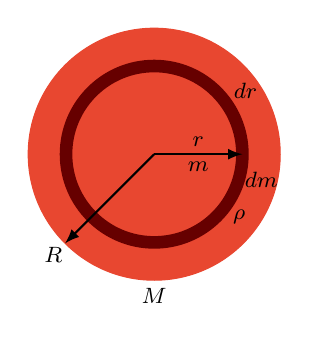
\begin{tikzpicture}[scale=.8]
            \filldraw[red!60!brown!90!] (0,0) circle (2cm);
            \draw[red!40!black,line width=1.6mm] (0,0) circle (1.4cm);
            \draw[-latex,thick] (0,0) -- (1.4,0);
            \draw[-latex,thick] (0,0) -- (-1.414,-1.414);
            \node at (1.45,1) {\footnotesize $dr$};
            \node at (1.7,-0.4) {\footnotesize $dm$};
            \node at (1.35,-1) {\footnotesize $\rho$};
            \node at (0.7,0.2) {\footnotesize $r$};
            \node at (0.7,-0.2) {\footnotesize $m$};
            \node at (-1.6,-1.6) {\footnotesize $R$};
            \node at (0,-2.25) {\footnotesize $M$};
        \end{tikzpicture}
    \end{figure}
\end{minipage}
\begin{minipage}{0.73\textwidth}
    \vspace{0.3cm}Ci chiediamo adesso quanta materia contiene un guscio stellare. Essa si può calcolare con l'equazione di continuità, ipotizzando che dentro il guscio sferico si conservi la massa (la densità è funzione del raggio)

    \begin{equation*}
        dm=4\pi r^2 \rho(r) dr
    \end{equation*}

    dove $\rho$ è la densità dello strato.
\end{minipage}

\vspace{0.2cm}In forma differenziale otteniamo la \textbf{prima equazione della struttura stellare}

\begin{equation}
    \frac{dm}{dr}=4\pi r^2 \rho(r)
    \label{struttura1}
\end{equation}

\subsubsection{Equilibrio idrostatico: seconda equazione di struttura stellare}

%\textbf{questa parte riascoltala perfavore sono gli ultimi 6 minuti}

\begin{minipage}{0.295\textwidth}
    \begin{figure}[H]
        \centering
        \begin{tikzpicture}
            \draw[blue!40!gray] (-1.3,0.5) .. controls (0,0.8) .. (1.3,0.5);
            \node[blue!40!gray] at (-1.8,0.5) {\footnotesize $r+ dr$};
        
            \draw[blue!40!gray] (-1.3,-0.5) .. controls (0,-0.2) .. (1.3,-0.5);
            \node[blue!40!gray] at (-1.8,-0.5) {\footnotesize $r$};
            
            \node[cylinder, draw, shape aspect=.5, cylinder uses custom fill, cylinder end fill=teal!40!gray, minimum height=0.4cm, cylinder body fill=teal!50!gray, %opacity=0.5,
            scale=3, rotate=90] at (0,0){};
        
            \draw[thick,red!40!gray,-stealth] (0.05,1.3) -- (0.05,0.6);
            \node[red!40!gray]  at (0.85,1.1)[red!40!gray] {\footnotesize $P(r + dr)$};
            \draw[thick,red!40!gray,-stealth] (0.05,-1.3) -- (0.05,-0.6);
            \node[red!40!gray]  at (0.5,-1.1)[red!40!gray] {\footnotesize $P(r)$};
            
            \draw[thick,-stealth] (-0.05,-0.2) -- (-0.05,-1.5) node [below] {gravità};
        \end{tikzpicture}
    \end{figure}
\end{minipage}
\begin{minipage}{0.7\textwidth}
    Si parla di equilibrio idrostatico quando la forza gravitazionale con cui un volume viene attratto dalla stella è pari alla variazione di pressione, cioè la pressione esercitata dagli strati inferiori su una shell deve essere uguale al contributo dato dalla forza gravitazionale della shell a cui si somma il contributo delle shell superiori.
\end{minipage}

La variazione di pressione con il raggio deve dunque essere uguale alla forza gravitazionale con cui un elemento di densità $\rho$ viene attratto al centro dalla sfera contenuta dentro $r$ che ha massa $m$.

\begin{equation*}
    -dPdA=\rho dAdr \frac{Gm(r)}{r^2}
\end{equation*}

Questo ci fa ottenere la \textbf{seconda equazione della struttura stellare}:

\begin{equation}
    \frac{dP}{dr}=-\frac{Gm(r)}{r^2}\rho(r)
    \label{struttura2}
\end{equation}

dove $r$ è la distanza dal centro dell'elemento di volume.

Nota: Noi sappiamo che se si ha una massa come quella in figura, ai fini della gravità conta solo la massa all'interno, non quella all'esterno, ecco perché abbiamo $r$ (teorema di Gauss).

Per risolvere questa equazione differenziale servono, come in tutte, delle condizioni al contorno. Le condizioni che assumiamo è che la pressione alla superficie sia nulla. L'approssimazione è lecita poiché questa pressione è molto bassa; del resto, incontra praticamente il vuoto esterno.

$$P_{sup}=0$$

Assumeremo inoltre che la massa al centro sia nulla (come se stessimo considerando la massa a $r=0$).

$$M_c=0$$

Così integrando l'equazione \ref{struttura2} da 0 a $R$ troveremo che la pressione al centro è\footnote{Per fare questa integrazione è il caso di considerare $m=m(r)$, dove poi avremo $\frac{m(r)}{M}=\frac{r^3}{R^3}$.}

$$P_c \simeq G \frac{{M_{\odot}}^2}{R^4}\simeq 10^{15} \; \rm Pa$$

Il calcolo di per sè non è esatto perché dovrebbe essere maggiore di un ordine di grandezza, ma almeno può essere utile a darci un'idea della pressione all'interno di una stella dati la sua massa e il suo raggio.

Cerchiamo di capire l'importanza delle forze di pressione, chiedendoci in quanto tempo collasserebbe il Sole su stesso "spegnendo" le forze di pressione. Questo tempo sarà dato, all'incirca, dal raggio diviso la velocità di fuga dalla superficie della stella

$$\tau_{dyn}=\frac{R}{v_{esc}}$$

dove

$$v_{esc}=\sqrt{\frac{2GM}{R}}$$

Si ottiene che, nel Sole $\tau_{dyn}=1100 \; \rm s\sim 18 \; min$, pertanto il Sole collasserebbe in circa 20 minuti. Questa grandezza è definita \textit{scala temporale dinamica}. Da qui si evince che le forze di pressione sono estremamente importanti. % e che sostengono il Sole

\subsubsection{Scala temporale di Kelvin-Helmholtz e terza equazione di struttura stellare}
Ci si può chiedere per quanto tempo il Sole potrebbe irradiare se l'unica fonte di energia fosse quella gravitazionale. In altre parole, se il Sole non avesse nessuna forma di produzione dell'energia al suo interno, potrebbe essere sostenuto dall'energia gravitazionale\footnote{Quando l'oggetto collassa, le sue parti aumentano di velocità e dunque l'energia potenziale si converte in energia cinetica.}?

L'energia potenziale gravitazionale $U$ di una sfera di massa $M$ e raggio $R$, supponendola a densità costante, è pari a

$$U=\frac{3}{5}G\frac{M^2}{R}$$

A partire da questa possiamo calcolare la \textit{scala temporale di Kelvin-Helmholtz}: essa è il tempo per cui una stella può brillare ad una certa luminosità $L$ data un'energia potenziale:

$$\tau_{\rm KH}=\frac{U}{2L}=\frac{\frac{3}{10}G\frac{M^2}{R}}{L}$$

(Nota: tale tempo è propriamente definito come il rapporto tra l'energia totale e la luminosità, ma per il teorema del viriale l'energia totale è metà di quella potenziale.)

Nel caso del Sole, sostituendo i dati si trova che il Sole potrebbe brillare per 30 milioni di anni, ma chiaramente il Sole esiste da molto più tempo.

Dunque serve una ulteriore fonte di energia. Ma prima di chiederci quale sia questa fonte, chiediamoci come l'energia si trasferirebbe nel Sole.

Supponiamo che tale fonte abbia una simmetria centrale, trovandosi entro una sfera di raggio $r$: da questa avremo un flusso di fotoni\footnote{Lo deduciamo dal fatto che è ciò che vediamo alla superficie.}. Ogni shell interna del Sole vede il passaggio di una certa quantità di fotoni e noi possiamo misurare tale flusso nell'ultimo strato e quindi potremo dire quanto ne è stato assorbito. 

Quando un flusso di fotoni attraversa uno strato, vedremo una diminuzione del numero di fotoni; come per le atmosfere stellari, si può immaginare che tale calo di fotoni sia una percentuale di ciò che è entrato:

$$\frac{dF}{F}=-\rho\kappa dr$$

Questa è la variazione di flusso della radiazione a causa dell'assorbimento in una shell di spessore \textit{dr}. Il meno è dovuto alla decrescita. $\kappa$ rappresenta l'assorbimento.

Qui stiamo supponendo che l'opacità non dipenda dalla frequenza: l'ipotesi è legittimata dal fatto che a temperature alte la principale fonte di assorbimento è attribuibile allo scattering Thomson, che non dipende dalla frequenza. Chiaramente negli strati più esterni (atmosfera) non sarà più vero, ma negli strati pù interni ha senso. Eventualmente si può introdurre un coefficiente di opacità medio.

Bisogna inoltre sapere come la propagazione dei fotoni contribuisca al sostegno della struttura: i fotoni assorbiti dalla shell impartiscono a questo strato un impulso; tale impulso per unità di tempo e di area è dato da $p=\frac{|F|}{c}$.

Il rate di incremento dell'impulso deve essere uguale alla forza netta applicata allo strato dal campo di radiazione, per la seconda legge di Newton. Questa quantità sarà riconducibile alla differenza di pressione di radiazione che il flusso di fotoni imprime alla shell (sempre per unità di area e di tempo):

\begin{equation}
    \frac{dP_{\rm rad}}{d \tau}=\frac{F}{c}
\end{equation}

dove $\tau=-\kappa \rho r$, da cui

\begin{equation}
    \frac{dP_{\rm rad}}{d r}=-\frac{\kappa \rho F}{c}
\end{equation}

%Sostituiamo $dF$ dall'espressione precedente e ricordiamo che

Abbiamo visto che in condizioni di equilibrio termodinamico locale (perché man mano che ci si addentra più il campo diventa isotropo e le condizioni di LTE sono valide) la pressione si può esprimere come (Eq. \eqref{eq:press_rad_eq_term})

$$P_{\rm rad}=\frac{1}{3} aT^4$$

\comment{\rule[7pt]{\linewidth}{0.4pt}
Ricaviamo la relazione appena scritta\footnote{I passaggi di seguito svolti sono presi da \textit{Kartunnen - Fundamental astronomy}.}.

Consideriamo un recipiente di volume $V=\Delta x \Delta y \Delta z$ e supponiamo di avere all'interno $N$ particelle che non interagiscono tra loro, per cui la pressione sarà causata soltanto dalle collisioni tra le particelle con le pareti del recipiente. Quando una particella colpisce una parete perpendicolare all'asse $x$, la componente lungo $x$ della sua quantità, $p_x$, varia di $\Delta p=2p_x$. La particella ritornerà alla stessa parete dopo un tempo $\Delta t=\frac{2 \Delta x}{v_x}$. Quindi la pressione esercitata dalle particelle sulla parete (la cui area è pari a $A=\Delta y \Delta z$) vale

$$P=\frac{F}{A}=\frac{\sum \frac{\Delta p}{\Delta t}}{A}
=\frac{\sum p_x v_x}{\Delta x \Delta y \Delta z}
=\frac{N \langle p_x v_x \rangle}{V}$$

con $\langle p_x v_x \rangle$ valor medio.

La quantità di moto è $p_x=mv_x$ (dove $m=\frac{h \nu}{c^2}$ per i fotoni), dunque

$$P=\frac{Nm \langle v_x^2 \rangle}{V}$$

Supponiamo che le velocità delle particelle siano distribuite isotropicamente, allora $\langle v_x^2 \rangle=\langle v_y^2 \rangle=\langle v_z^2 \rangle$ e pertanto

$$\langle v^2 \rangle
=\langle v_x^2 \rangle=\langle v_y^2 \rangle=\langle v_z^2 \rangle
=3\langle v_x^2 \rangle$$

e

$$P=\frac{Nm \langle v^2 \rangle}{3 V}$$

Se le particelle sono molecole di un gas, l'energia di una molecola è $\varepsilon=\frac{1}{2}mv^2$. L'energia totale del gas sarà $E=N \langle \varepsilon \rangle=\frac{1}{2} N m \langle v^2 \rangle$, e la pressione può essere scritta come

$$P=\frac{2}{3} \frac{E}{V}$$

Se le particelle sono fotoni, essi si muovono alla velocità della luce e la loro energia è $\varepsilon=mc^2$. L'energia totale di un gas di fotoni sarà quindi $E=N \langle \varepsilon \rangle=Nmc^2$ e la pressione sarà

$$P=\frac{1}{3} \frac{E}{V}$$

D'altra parte, per un corpo nero la densità di corpo nero è

$$\frac{E}{V}=u=\frac{4\pi}{c} I
=\frac{4}{c} F
=\frac{4}{c} \sigma T^4
\equiv a T^4$$

dove $a=\frac{4 \sigma}{c}$ è la costante di radiazione. in definitiva la pressione è

$$P_{\rm rad}=a \frac{T^4}{3}$$

\rule[7pt]{\linewidth}{0.4pt}}

da cui derivando rispetto a $r$ otteniamo

$$\frac{dP_{\rm rad}}{dr}=\frac{4}{3} a T^3\frac{dT}{dr}$$

Inoltre ricordiamo che:

$$L=4\pi r^2 F(r)$$

dunque alla fine otterremo:

$$L=-\frac{16\pi r^2acT^3}{3\kappa \rho}\frac{dT}{dr}$$

la quale ci dice che la luminosità è proporzionale al gradiente di temperatura. Invertendo l'espressione otterremo la \textbf{terza equazione della struttura stellare}

\begin{equation}
    \frac{dT}{dr}=-\frac{3}{16 \pi ac}\frac{\kappa \rho}{T^3}\frac{L}{r^2}
    \label{struttura3}
\end{equation}

La terza equazione della struttura stellare ci dice che il gradiente di temperatura è legato alla luminosità, alla densità e alla temperatura, che sono parametri che conosciamo. Ma è anche legata all'opacità, che di fatto non conosciamo. Essa però può essere calcolata in tutti gli strati in base alla composizione chimica, temperatura e densità. Questa opacità quindi cambierà in ogni strato, ma facendo i calcoli si scoprirà che la variazione sarà piccola.

\vspace{0.2cm}L'equazione \ref{struttura3} andrà bene se i protagonisti del meccanismo di trasferimento dell'energia sono i fotoni. Ma se ci fossero altri meccanismi non basati sui fotoni?

\subsubsection{Convezione: quarta equazione di struttura stellare}

\begin{minipage}{0.365\textwidth}
    \begin{figure}[H]
        \centering
        \includegraphics[scale=0.5]{bolla.png}
        \label{bolla}
    \end{figure}
\end{minipage}
\begin{minipage}{0.63\textwidth}
    \vspace{0.6cm}Se nelle zone più interne la temperatura di una porzione di questo ambiente risulta più calda del resto, questa bolla salirà e si espanderà fino a raggiungere la temperatura dell'ambiente circostante. L'energia corrispondente sarà stata trasferita alla parte "in alto" dell'ambiente. Dovendosi conservare la materia, avremo un calo di un'altra bolla più fredda. Tale meccanismo di circolazione della materia è detto di \textit{convezione}.

    A questo punto ci si chiede quali siano le condizioni affinché ciò accada e quanta energia trasporta. Il fenomeno più efficiente tra la radiazione e la convezione è quest'ultimo, per cui se avviene questo meccanismo la stella si raffredderà più velocemente.
\end{minipage}

\vspace{0.2cm}\footnote{Questa parte è presa dalle lezioni del prof. Pirronello.}Supponiamo di essere all'interno della stella e supponiamo che l'elemento di fluido alla temperatura $T_{\rm int}$ (uguale alla temperatura esterna $T_{\rm ext}$) tenda a salire verso l'alto di un tratto infinitesimo $dr$. Salendo, si dirige verso zone a pressione minore, quindi si espande per equilibrare quest'ultima.

Dopo che è salito, si avrà $T'_{\rm int} \neq T'_{\rm ext}$, però ovviamente $P_{\rm int}=P_{\rm ext}$ ad ogni livello. La temperatura del volumetto si differenzia sempre più da quella dell'ambiente circostante, dunque l'espansione è adiabatica per ogni intervallo di tempo.

Affinché questo fluido continui a salire, esso deve trovarsi in una zona la cui densità esterna è maggiore di quella interna per via del principio di Archimede, quindi

$$\left| \frac{d\rho}{dr} \right|_{\rm ext}<\left| \frac{d\rho}{dr} \right|_{\rm int}$$

dove i valori assoluti sono usati perché, considerando che il fluido si muove verso l'alto, si muove verso regioni a pressione, densità e temperatura minore in quanto i gradienti sono rivolti verso il basso, quindi $\frac{d\rho}{dr}$ sarebbero negativi.

L'espressione quindi ci dice che la densità all'interno varia più velocemente di quanto varia all'esterno, così mentre l'elemento di fluido si sposta verso l'alto rimane a densità minore rispetto all'esterno. Si avrà allora

$$-\left| \frac{d\rho}{dr} \right|_{\rm ext}>-\left| \frac{d\rho}{dr} \right|_{\rm int}
\implies
\left. \frac{d\rho}{dr} \right|_{\rm ext}>\left. \frac{d\rho}{dr} \right|_{\rm int}$$

%tale condizione è detta \textbf{criterio di Schwarzschild}.

Facciamo una valutazione di quando questo meccanismo si verifica.

\begin{itemize}
    \item \textbf{Fuori dalla bolla}
    
    Supponendo che valga l'equazione dei gas perfetti, essa fornisce
    $$P=\frac{k_B}{\overline{m}}\rho T$$
    dove $\overline{m}=\mu m_{\rm H}$. Derivando:
    $$\frac{dP}{dr}\bigg|_{\rm ext}=\frac{k_B}{\overline{m}}T\frac{d\rho}{dr}+\frac{k_B}{\overline{m}}\rho \frac{dT}{dr}$$
    Dall'equazione dei gas perfetti si hanno:
    $$\frac{k_B}{\overline{m}}T=\frac{P}{\rho}\qquad \frac{k_B}{\overline{m}}\rho=\frac{P}{T}$$
    Sostituendo avremo:
    $$\frac{dP}{dr}\bigg|_{\rm ext}=\frac{P}{\rho}\frac{d\rho}{dr}\bigg|_{\rm ext} + \frac{P}{T}\frac{dT}{dr}\bigg|_{\rm ext}$$
    da cui invertendo
    $$\left. \frac{d\rho}{dr} \right|_{\rm ext}
    =\frac{\rho}{P}\left. \frac{dP}{dr} \right|_{\rm ext} - \frac{\rho}{T}\frac{dT}{dr}\bigg|_{\rm ext}$$
    \item \textbf{Dentro la bolla}
    
    \E ragionevole pensare che l'espansione della bolla sia adiabatica, da cui:
    $$P=k\rho^\gamma$$
    Derivando:
    $$\frac{dP}{dr}\bigg|_{\rm int}
    =k\gamma\rho^{\gamma-1}\frac{d\rho}{dr}
    =\gamma k\frac{\rho^\gamma}{\rho}\frac{d\rho}{dr}\bigg|_{\rm int}
    =\gamma\frac{P}{\rho}\frac{d\rho}{dr}\bigg|_{\rm int}$$
    da cui
    $$\left.\frac{d\rho}{dr} \right|_{\rm int}
    =\frac{1}{\gamma} \frac{\rho}{P} \left. \frac{dP}{dr} \right|_{\rm int}$$
\end{itemize}

%\textbf{sta frase non so dove metterla}Avremo quindi un gradiente \textit{radiativo}, relativo all'esterno, in cui scorrono i fotoni; e un gradiente \textit{adiabatico}, relativo all'interno della bolla.

Sostituendo nella legge di Archimede avremo

$$\frac{1}{\gamma} \frac{\rho}{P} \left. \frac{dP}{dr} \right|_{\rm int} < \frac{\rho}{P}\left. \frac{dP}{dr} \right|_{\rm ext} - \frac{\rho}{T}\frac{dT}{dr}\bigg|_{\rm ext}$$

Mentre densità e temperatura variano tra l'interno e l'esterno in maniera considerevole, lo stesso non avviene per le pressioni: il fluido infatti si espande per bilanciare la pressione esterna. Allora, possiamo dire che le pressioni strato per strato si
equilibrano velocemente e dunque

$$\left. \frac{dP}{dr} \right|_{\rm ext}
=\left. \frac{dP}{dr} \right|_{\rm int}
\equiv \frac{dP}{dr}$$

Quindi si ottiene

$$\left. \frac{dT}{dr} \right|_{\rm ext} < \frac{T}{P}\left(1-\frac{1}{\gamma}\right)\frac{dP}{dr}$$

il secondo termine è le derivata logaritmica di $T=k P^{\frac{\gamma - 1}{\gamma}}$ (cioè è pari al rapporto tra la derivata della funzione e la funzione stessa), che è la seconda equazione di Poisson per le adiabatiche. Dunque

$$\left. \frac{dT}{dr} \right|_{\rm adi}
=\left. \frac{dT}{dr} \right|_{\rm int}
>\left. \frac{dT}{dr} \right|_{\rm ext}$$

%Essendo nelle condizioni limite dove il fluido diventa instabile per convezione si ha che
Supponendo che fuori dalla bolla il trasporto di energia avvenga solo per radiazione si ha

$$\left. \frac{dT}{dr} \right|_{\rm ext}=\left. \frac{dT}{dr} \right|_{\rm rad}$$

%\textbf{da qui inizia la parte che spiega lui}

%Imponendo che le pressioni siano uguali nel punto di raccordo tra l'esterno e l'interno (qui si fermerà il processo), eguagliando le $\frac{dP}{dr}$ avremo la condizione in cui il "processo si arresta"

%$$\frac{dT}{dr}=\frac{T}{P}\left(1-\frac{1}{\gamma}\right)\frac{dP}{dr}$$

%Essa ci dà un confronto tra la variazione all'esterno della bolla e quella all'interno della bolla \textbf{Sicuro?}.

%Unendo questa espressione con la \ref{struttura2} e l'equazione dei gas perfetti si ha

%$$\frac{dT}{dr}\bigg|_{\rm adi}=-\left(\frac{\overline{m}}{k_B}\right)\left(1-\frac{1}{\gamma}\right)\frac{GM}{r^2}$$



Se la temperatura scende nell'ambiente più rapidamente di quanto non faccia nella bolla, ossia se il gradiente esterno è maggiore di quello interno, si instaura un regime di instabilità che porta alla convezione. Per quanto detto prima si avrà

$$\frac{dT}{dr}\bigg|_{\rm rad} > \frac{dT}{dr}\bigg|_{\rm adi}$$

che è detto \textbf{criterio di Schwarzschild}. Quando accade questo fenomeno, cioè quando vediamo questo moto di massa per portare la temperatura rapidamente a zero (o valori più bassi) negli strati esterni? Quando i fotoni non riescono ad uscire, cioè quando si ha alta opacità rispetto allo strato più esterno.

Ci chiediamo allora perché negli strati più esterni l'opacità diventa bassa. Osservando infatti la superficie del Sole ci accorgiamo che ci sono piccole bolle di convezione, dunque è lecito pensare che il Sole non sia interamente convettivo.

Quello che accade, probabilmente, è che negli strati più esterni, dove dovrebbe avvenire la convezione, si hanno temperature più basse e dunque avvengono transizioni legato-legato, nelle quali i fotoni vengono assorbiti. Allora l'energia del campo di radiazione sarà convertita in cinetica, comportando il riscaldamento della materia che instaurerà un processo convettivo.

Abbiamo chiarito le condizioni per cui si crea convezione: adesso bisogna chiarire quanta energia viene trasportata. Il problema si può scindere in due parti:

\begin{itemize}
    \item Sapere quanta energia riesce a immagazzinare un elementino di volume (in flusso). Essa è data da
    $$F_{\rm conv}=\rho v dQ=\rho vC\Delta T$$
    dove $C$ è la capacità termica e $\Delta T$ è la differenza di temperatura tra la temperatura dello strato in cui la bolla comincia la sua instabilità e quella in cui si termalizza.
    \item Sapere con quale velocità un elementino di volume si muove.
\end{itemize}

L'ultimo dei due punti evidenziati presenta una criticità: ci serve un modello della convezione che permetta di stimare la velocità $v$ delle celle convettive. Includendo la rotazione delle stelle, questo è un problema tridimensionale.

Esistono delle rappresentazioni empiriche in cui si presume che le bolle abbiano una percorrenza che dipende dalla scala di pressione. Qui si parla di una sorta di lunghezza di rimescolamento, che è un parametro che è stato assunto sulla base di osservazioni e quindi il modello non è pienamente soddisfacente.

\vspace{0.2cm}Chiediamoci adesso quale sia il modo per introdurre la generazione di energia all'interno di una stella.

La prima idea è immaginare che tale energia venga prodotta in una percentuale della massa stessa, il che non è assurdo considerando che più massa c'è, più energia può essere generata. Possiamo supporre che la luminosità sia proporzionale alla massa, ovvero

$$L\propto 4\pi r^2\rho dr$$

Introduciamo un coefficiente di proporzionalità $q$ che è il \textit{rate di generazione di energia} per unità di massa

\begin{equation}
   \frac{dL}{dr}=4\pi r^2\rho q
    \label{struttura4} 
\end{equation}

Questa è la \textbf{quarta equazione della struttura stellare}, sotto l'ipotesi di essere in equilibrio termodinamico.

\vspace{0.2cm}Le quattro equazioni appena ricavate codificano il problema della struttura stellare. Ad esse vanno affiancate l'equazione di stato dei gas, un'equazione dell'opacità e il coefficiente di assorbimento dell'energia.

\subsubsection{Che tipo di energia? Fusione nucleare}
Trattando la scala temporale di Kelvin-Helmholtz abbiamo visto che l'energia gravitazionale non sarebbe sufficiente a mantenere il Sole con la luminosità che conosciamo per un certo periodo di tempo.

Il processo più efficiente per la produzione di energia è la \textit{fusione nucleare}.

Per esempio, se da quattro nuclei di H si genera un nucleo di He, avremo un difetto di massa che corrisponde a un'energia $\Delta E=27$ MeV. Questi processi di fusione sono reazioni esoenergetiche. Infatti come già sappiamo tutte le reazioni verso il ferro sono esoenergetiche quindi nelle stelle per fusione si possono ottenere tutti gli elementi fino al ferro. Dato che l'H domina nella composizione, è ragionevole pensare che il meccanismo primario per la produzione di energia sia la fusione di idrogeno.

Ma rimane il problema del fatto che i nuclei di idrogeno, avendo la stessa carica elettrica, si pensa che non riescano a raggiungersi in distanze dell'ordine del raggio atomico. La temperatura affinché la velocità sia tale da raggiungere questa condizione è dell'ordine di $10^{10}$ K.

$$E=\frac{3}{2}k_B T \qquad E
=\frac{1}{4\pi \varepsilon_0}\frac{e^2}{r_0}$$
$$T=\frac{1}{6\pi k_B \varepsilon_0}\frac{e^2}{r_0}\simeq 10^{10} \rm K$$

Proviamo a stimare la temperatura centrale del Sole; conosciamo la densità media e la pressione al centro, ponendo $\myol{\mu}$ uguale al peso medio molecolare (per l'idrogeno ionizzato è circa 0.5), usando l'equazione dei gas perfetti avremo

$$T_c=\frac{\Bar{\mu}m_H}{\Bar{\rho}}\frac{P_c}{k_B}\simeq 10^7 \rm K$$

Dunque il Sole non è abbastanza caldo.

Il quesito fu risolto guardando al processo del decadimento $\alpha$, che è il processo inverso.

Gamow suppose che si riesce a superare la barriera classica del potenziale coulombiano grazie al fenomeno dell'effetto tunnel. La probabilità che una particella con velocità $v$ superi la barriera è data da

$$P(v)=e^{-2\pi \eta}
\quad\text{dove}\quad
\eta=\frac{1}{4\pi \varepsilon_0}\frac{Z_1Z_2}{\hbar v}$$

La distribuzione maxwelliana di velocità è

$$t(v)=\left( \frac{m}{2\pi k_B T} \right)^{3/2}4\pi v^2 e^{-\frac{mv^2}{2k_BT}}$$

dunque la probabilità di avere la velocità che ci serve sarebbe molto più bassa. Considerando l'effetto tunnel invece la probabilità è non nulla

$$P\propto e^{(-T/T_0)^{-1/3}}\quad T_0=\left( \frac{3}{2} \right)^3\left( \frac{4\pi^2 Z_1Z_2}{h} \right)^2\left( \frac{m}{k_B} \right)$$

per cui si avrà un numero di reazioni sufficientemente alto per avere un rate di produzione di energia come quello osservato dalla luminosità

\begin{figure}[H]
    \centering
    \includegraphics[width=8cm]{prob.png}
\end{figure}

Il picco di Gamow in figura rappresenta l'energia alla quale avverrà la reazione. Esso è dato dal prodotto della maxwelliana per la probabilità di penetrazione.

\subsubsection{Reazioni più frequenti}
Naturalmente le reazioni più frequenti sono quelle che coinvolgono H e He, cioè gli elementi maggiormente presenti.
\begin{itemize}
    \item \textbf{Ciclo protone-protone (PP)}: due nuclei di idrogeno danno origine a un deuterio con l'emissione di un positrone e di un neutrino
    $$\ce{_1^1H + _1^1H -> _1^2H + _1^0\myol{\textit{e}} + _0^0\nu}$$
    Il deuterio può unirsi ad un altro idrogeno, dando luogo $\ce{_2^3He}$ ed emettendo un $\gamma$ (quindi un fotone)
    $$\ce{_1^2H + _1^1H -> _2^3He + + _0^0\gamma}$$
    A loro volta due atomi di $\ce{_2^3He}$ possono dare luogo ad $\ce{_2^4He}$ e a due nuovi atomi di idrogeno che rientrano nel ciclo
    $$\ce{_2^3He + _2^3He -> _2^4He + _1^1H + _1^1H}$$
    \item \textbf{Ciclo CNO}: ove fossero presenti C, N, O, essi fungono da catalizzatori e non vengono alterati in abbondanza
    \begin{eqnarray*}
        \ce{_6^{12}C + _1^1H -> _7^{13}N + _0^0\gamma}\\
        \ce{_7^{13}N -> _6^{13}C + _1^0\myol{\textit{e}} + _0^0\nu}\\
        \ce{_6^{13}C + _1^1H -> _7^{14}N + _0^0\gamma}\\
        \ce{_7^{14}N + _1^1H -> _8^{15}O + _0^0\nu}\\
        \ce{_8^{15}O -> _7^{15}N + _1^0\myol{\textit{e}} + _0^0\nu}\\
        \ce{_7^{15}N + _1^1H -> _6^{12}C + _2^4He}
    \end{eqnarray*}
    \item \textbf{Ciclo 3$\boldsymbol{\alpha}$}: due nuclei di elio si uniscono per formare un berillio e producendo un $\gamma$
    $$\ce{_2^4He + _2^4He -> _4^8Be + _0^0\gamma}$$
    Il berillio incontra un altro atomo di elio e produce un carbonio e un $\gamma$
    $$\ce{_4^8Be + _2^4He -> _6^{12}C^* + _0^0\gamma}$$
\end{itemize}

\begin{figure}[H]
    \centering
    \includegraphics[scale=0.7]{reazioni.png}
\end{figure}

Queste reazioni avvengono con varie probabilità: la catena PP è possibile a basse temperature, quando ancora H e C non riescono a fondersi (il picco di Gamow è spostato a temperature più alte); nel caso del Sole (di cui si stima una temperatura del nucleo pari a 15 milioni di gradi) è possibile. A queste temperature è anche possibile che avvenga il CNO ma con minore efficienza. Infatti l'energia prodotto dal ciclo PP ha un andamento che va con $T^4$, quella del ciclo CNO va come $T^{18}$ La $3\alpha$ invece avviene a temperature molto più alte.

Nota: La radiazione che noi vediamo è prodotta a partire dai $\gamma$. Noi però vediamo lo spettro nel visibile: i fotoni devono attraversare il Sole interagendo con la materia e trasferendole energia; ciò porta a una termalizzazione del campo di radiazione fino ad avere un ambiente dove vale l'equilibrio termodinamico locale. Quindi noi vedremo la planckiana che ha quella temperatura e non lo spettro piccato dei fotoni.

\subsubsection{Risoluzione delle equazioni di struttura stellare}
Le equazioni trovate nei paragrafi precedenti sono risolubili solo numericamente e dipendono da una serie di ipotesi.

Per le soluzioni analitiche bisogna assumere che il Sole sia un politropo, cioè che la pressione vada con densità elevata a $\gamma$.

Numericamente invece la soluzione dipende dalla massa della stella e la sua composizione chimica.

Come condizioni al contorno poniamo

$$\begin{cases}
    M(r=0)=0\\
    L(r=0)=0\\
    \rho(\text{superficie})=\rho(\text{fotosfera})\\
    T(\text{superficie})=T(\text{fotosfera})
\end{cases}$$

In particolare le ultime due quantità possono considerarsi zero perché piccole rispetto a $\rho(0)$ e $T(0)$ (tali grandezze sono massime al centro). Inoltre per superficie non si intende solo lo strato più esterno ma gli strati più esterni. Si assume inoltre che la composizione chimica della stella sia quella osservata.

Ci serviranno due parametri: il coefficiente di opacità e quello di produzione di energia (precedentemente indicato con $q$, d'ora in poi potremmo trovarlo con $\varepsilon$). Si useranno anche le equazioni di stato.
Se si mettessero delle ipotesi diverse, le equazioni si potrebbero anche integrare (per esempio con un'opacità meno dettagliata).

I risultati ottenuti sono i seguenti:

\begin{figure}[H]
    \centering
    \includegraphics[scale=0.7]{soluzioni.png}
    %\caption{Soluzioni delle equazioni di struttura}
\end{figure}

\subsubsection{E se fosse tutto un'invenzione? I neutrini solari}
E se tutto quello che abbiamo detto fin ora fosse un'invenzione? Il dubbio è ragionevole perché non esiste la prova che queste equazioni abbiano soluzione unica.

Le oscillazioni solari (variazioni di luminosità in periodi molto brevi), che hanno un periodo di circa 6 minuti, impongono che il Sole sia una cavità e quindi corroborano la nostra tesi.

Un'altra prova sta nel fatto che per tale modello abbiamo bisogno di una certa energia: tale produzione di energia, oltre a produrre i fotoni che sostengono la struttura del Sole, produce anche neutrini. Tale fatto è una verifica del modello scorporata dal modello stesso

$$\ce{4p -> _2^4He + 2 e^{+} + 2 \nu_e}$$

I neutrini riescono a quasi non interagire con la materia e, quando furono misurati per la prima volta, erano 1/3 di quelli attesi, poi in realtà si capì che il neutrino cambia nel raggiungere la Terra. Le misure sono state realizzate con il Super Kamiokande, un telescopio di neutrini solari che sfrutta la radiazione Cherenkov dei neutrini in acqua.

\subsection{Estensione del modello dal Sole alle altre stelle}
Come facciamo a estendere il calcolo della struttura al resto delle stelle? Il Sole è un oggetto di cui conosciamo tutte queste informazioni perché è vicino; in generale, per verificare un modello, ci servirebbe quanto meno capire se alla superficie c'è una consistenza dei vari parametri (ad es massa, raggio, luminosità).

Gli unici oggetti che possono essere utilizzati sono i sistemi binari, costituiti da due stelle che orbitano. La percentuale di questi sistemi è consistente: per le stelle di grande massa sono binari circa il 50\% di tali sistemi, per quanto riguarda le stelle come il Sole ci aggiriamo intorno al 44\%.

Per i sistemi binari ci è possibile misurarne il periodo di rotazione e la masse, ma si possono ottenere anche degli spettri: si ottengono delle righe spettrali che però sono soggette ad effetto Doppler, e quindi mostreranno uno shift positivo e uno negativo in maniera periodica.

\begin{figure}[H]
    \centering
    \includegraphics[scale=0.3]{doppler.png}
    %\caption{Qui si vedono gli shifting in base all'effetto Doppler dovuto al moto}
\end{figure}

La spettroscopia, come abbiamo visto in maniera ampia, ci permette di ottenere parametri come la temperatura e il raggio. Il raggio può essere misurato anche mediante fenomeni di eclissi.

\subsubsection{Stelle di sequenza principale}

Risolvendo l'equazione della struttura stellare per una stella dominata da idrogeno, veniva fuori la sequenza principale del diagramma H-R.

Ciò fa pensare che l'impianto sia corretto. Ci possono essere anche degli errori, poiché bisogna ricordare le approssimazioni che abbiamo fatto in origine.

Supponendo anche di conoscere la massa e la luminosità di un sistema di stelle, le misure si allineano con la seguente relazione

$$L\propto M^{3.5}$$

Tale relazione osservativa può essere utilizzata come un test della bontà delle
equazioni per la struttura interna delle stelle.

Dall'equazione dell'equilibrio idrostatico \eqref{struttura2} si ha, ponendo $\rho=\frac{M}{R^3}$ e integrando in $dr$ tra $0$ e $R_s$:

\begin{gather*}
    -P_c= \int_{0}^{R_s} dP
    =-\int_{0}^{R_s} \frac{Gm(r)}{r^2}\rho(r)dr
    \simeq -G\frac{4\pi\rho^2}{3} \int_{0}^{R_s} r \, dr \simeq
    \\
    \simeq -\frac{1}{2} \frac{G \rho M}{R}\\
    \implies P_c\propto G\frac{M^2}{R^4}
\end{gather*}

Inoltre, dall'equazione di stato si può ottenere

\begin{equation*}
    T\propto \frac{P}{\rho}
    \implies
    T_c\propto \frac{M^2}{R^4}\frac{R^3}{M}=\frac{M}{R}
\end{equation*}

Andando a sostituire nell'equazione \ref{struttura3} otteniamo

$$\frac{M}{R^2}\propto \frac{\frac{M}{R^3}}{R^2\left( \frac{M}{R} \right)^3}L\implies L\propto M^3$$

Come vediamo, le nostre ipotesi rispecchiano quasi esattamente i dati sperimentali. Tutto ciò vale per le stelle che bruciano idrogeno.

\subsubsection{Stelle di massa simile al Sole}

Supponendo che bruci solo idrogeno (catena PP) si ottengono i seguenti risultati per temperatura e densità:

\begin{figure}[H]
    \centering
    \includegraphics[scale=0.6]{tempdens.png}
\end{figure}

Il modello da noi calcolato dice che, da un certo punto in poi, non si ha più trasporto radiativo ma convettivo: la temperatura al centro è alta e i fotoni riescono a passare, poi la temperatura scende e si ha una ricombinazione della materia tale da fare aumentare l'opacità e impedire il passaggio di fotoni.

Dunque è ragionevole supporre che, per stelle che vanno dalle 0.5 alle 1.5 masse solari, si abbia un \textit{core} radiativo e un involucro convettivo.

\begin{figure}[H]
    \centering
    \includegraphics[scale=0.5]{solecore.png}
\end{figure}

\subsubsection{Nane brune}
Se la massa della stella è $M<0.08 M_{\odot}$, non brucia più l'idrogeno (serve una temperatura minima affinché il bruciamento di idrogeno sia efficiente a sostenere la struttura stellare e quindi anche una massa minima). Per masse tali che

$$0.013 M_{\odot}<M<0.08 M_{\odot}$$

può bruciare il deuterio. Tali stelle prendono il nome di \textit{nane brune.} Sono stelle di tipo spettrale L-T \textit{molto late} (con "late" letto in inglese), cioè di temperatura bassa. Sono poco visibili e se ce ne dovessero essere tante potrebbero spiegare alcune anomalie riguardanti la galassia (come per esempio la massa che non riusciamo a trovare). Si trovano in basso a destra nel diagramma H-R.

\subsubsection{Stelle con massa inferiore a 0.5 masse solari}

Su queste stelle, ciò che si può dire è che la temperatura è così bassa che i fotoni non sono efficienti come sistemi di trasferimento di energia: tutta la stella è convettiva.

\subsubsection{Stelle di massa elevata, in particolare superiore a 1.5 masse solari}

Da queste equazioni si vede che esiste un limite inferiore alla massa delle stelle, che consente il bruciamento dell'idrogeno. Di contro esiste anche un limite superiore alla massa delle stelle, dato dalla pressione di radiazione. Questa pressione può trasferire impulso alla materia e spingerla fuori. Affinché ci sia equilibrio serve che la pressione di radiazione non superi il contributo gravitazionale, dunque

$$aT^4 \leq G\frac{Mm}{r^2}$$

Supponendo che la stella bruci idrogeno e considerando dominante lo scattering Thomson, si può stabilire il cosiddetto \textit{limite di Eddington}, che afferma che la massa di una stella deve soddisfare la relazione

$$M<90M_{\odot}$$

altrimenti la temperatura al centro sarebbe così elevata da produrre un flusso di fotoni tale da spazzare via la stella stessa.

Ciò non significa che oggi non siano state identificate stelle più massive, ma sono stelle evolute dove non si brucia più idrogeno.

\subsubsection{Classificazione sommaria delle stelle}
Ricapitolando: 
\begin{itemize}
    \item Per stelle con massa $M<0.5 M_{\odot}$ la temperatura è così bassa in tutta la stella che i fotoni non sono efficienti come sistema di trasferimento dell'energia, per cui la stella è interamente convettiva (stelle rimanenti, in particolare le stelle L, T rientrano nelle nane brune).
    \item Per stelle con massa $0.5M_{\odot}<M<1.5 M_{\odot}$ come il Sole il nucleo radiativo, involucro convettivo (stelle F, G, K);
    \item Per le stelle con $M>1.5M_{\odot}$, la produzione di energia nel \textit{core} è così elevata da creare un enorme flusso di fotoni, talmente alto che non riescono a uscire e la materia assorbe tutto quel che viene prodotto: il nucleo è convettivo. Nella parte più esterna invece si ha un meccanismo radiativo. Incide anche la differenza di densità di materia su una stella di grande massa: qui gli elettroni sono vicinissimi tra di loro (stelle O, B, A e parte delle F);
\end{itemize}

\begin{figure}[H]
    \centering
    \includegraphics[scale=0.8]{hr_core.png}
    \label{fig:my_label}
\end{figure}

Il diagramma H-R si può anche così schematizzare, in base alla luminosità:

\begin{itemize}
    \item \textit{Giganti}: sono stelle di grande luminosità e vanno dalla classe di luminosità III a I. Si possono suddividere ulterioremente in:
    \begin{itemize}
        \item \textit{Supergiganti}: classe I;
        \item \textit{Giganti brillanti}: classe II;
        \item \textit{Giganti}: classe III;
    \end{itemize}
    \item \textit{Subgiganti}: sono di classe IV, rappresentano la via di mezzo tra giganti e sequenza principale;
    \item \textit{Sequenza principale}: classe V;
    \item \textit{Nane bianche}: sono stelle con bassa luminosità e altissima densità.
\end{itemize}


\subsection{Evoluzione stellare}
Il modello sin ora discusso non è in grado di spiegare le giganti e le nane. Questo perché le reazioni nucleari che abbiamo analizzato fin adesso inducono un cambiamento della composizione chimica, quindi è come se dovessimo risolvere le equazioni della struttura stellare assumendo una certa composizione chimica e, dopo aver trovato una soluzione, ammettere che tale composizione è cambiata e quindi dover ricalcolare tutto. Ciò è necessario poiché ci sono svariate reazioni nucleari.

Quando cambia la composizione chimica cambiano sia la densità che l'opacità, quindi servono una nuova $\rho$ e una nuova $\kappa$. Ad ogni istante, dovremmo capire come cambia la composizione chimica e quindi dobbiamo chiederci quali sono tutti i possibili processi che riescono a trasformare gli atomi (per esempio aggiungendo protoni e neutroni possiamo cambiare l'atomo, oppure può esserci fotodisintegrazione\footnote{Fotodisintegrazione di tutti i nuclei pesanti: la temperatura diventa così alta che i
fotoni termici sono in grado di spaccare tutti i nuclei pesanti presenti nel nucleo stellare,
ritrasformandoli in protoni e neutroni.}).

Quello che si fa è partire con una certa composizione chimica a $t=t_0$, troviamo l'equilibrio, calcoliamo le conseguenze delle reazioni nucleari e poi ricalcoliamo il modello a $t=t_1$ con la nuova composizione chimica e così via in maniera iterativa. Poiché la stella cambia nel tempo, si parla dunque di \textit{evoluzione stellare}.

Ci chiediamo allora se effettivamente possiamo spiegare l'evoluzione stellare in termini di evoluzione chimica.

Partiamo dall'evoluzione di stelle di massa piccola, come il Sole. Noi conosciamo l'andamento di temperatura e densità e sappiamo che ha un nucleo radiativo e un inviluppo convettivo. L'elio che si produce nel nucleo, essendo più pesante dell'idrogeno, si addenserà al centro creando una zona di altissima densità (il core), dunque apparentemente sta scendendo la pressione (chiaramente non è possibile perché la pressione del nucleo di elio deve essere uguale alla pressione dell'ambiente di idrogeno attorno). L'idrogeno, a questo punto, sta bruciando attorno a questa zona.

%Come cambia una stella in cui accade tutto ciò? Già le dimensioni diminuiscono poiché la parte di elio, poiché la parte di elio si contrae.
Cosa accade? L'idrogeno brucia inizialmente al centro, dove la temperatura è più alta, poi man mano in shell più lontane e quindi la produzione di energia si sposta verso l'esterno, tanto che la stella diventa più luminosa e aumenta un po' la temperatura. Quello che succede nel diagramma è che la stella, man mano che brucia idrogeno e lo converte in elio, diventa un oggetto di temperatura e luminosità sempre maggiori.

\vspace{0.2cm}Per quanto riguarda stelle con masse alte, con nucleo convettivo, l'idrogeno non vede l'elio accumularsi, ma si mischiano a causa della convezione, dunque il bruciamento dell'idrogeno non avviene in una shell che circonda un nucleo di elio, ma avverrà nello stesso spazio. Quindi quello che accade è che si ha una variazione della pressione all'interno del nucleo che coinvolge tutto la regione in cui avviene il bruciamento e si ha un aumento dell'elio. Dopo un certo tempo tutta la zona convettiva si sarà convertita.

Dunque, mentre prima si aveva un aumento di luminosità e temperatura dell'oggetto, in questo caso tutta la regione di bruciamento rimarrà inalterata (subirà una compressione a causa della trasformazione in elio) e qui si ha una diminuzione della temperatura nonostante un aumento della luminosità.

\subsubsection{Vita nella sequenza principale}
Quanto tempo una stella rimane in sequenza principale dipende dalla sua massa. Se immaginiamo che tale durata dipende dalla capacità di convertire la massa della stella in luminosità secondo un coefficiente di efficienza $f$

$$t=\frac{fMc^2}{L}$$

Ricordando inoltre che $L\propto M^{3.5}$, andando a sostituire otterremo

$$t\propto M^{-2.5}$$

dunque una stella rimane in sequenza principale tanto meno quanto più è massiva. Per esempio, il Sole con questo calcolo dovrebbe rimanere nella sequenza principale 12 miliardi di anni; una stella con massa pari a metà di quella del Sole permarrà nella sequenza principale per 70 miliardi di anni; infine, una stella di massa pari a 25 masse solari rimane nella sequenza principale per 4 milioni di anni, per questo ce n'è poche. Quindi più è piccola una stella, meno energia consuma.

Quello che noi immaginiamo dovesse essere, nel diagramma H-R, la posizione delle stelle di puro idrogeno, è una linea che viene detta \textit{zero age main sequence} (ZAMS), perché immaginiamo che siano appena nate. Lo spessore della sequenza principale è dovuto all'invecchiare delle stelle, infatti le stelle calde hanno una maggiore dispersione, quelle di piccola massa sono alla ZAMS. La maggiore dispersione delle stelle calde che noi conosciamo è detta \textit{terminal age main sequence.} 

%Ciò che succede alle stelle che esauriscono l'idrogeno al nucleo sarà oggetto della prossima lezione (evoluzione di post-sequenza).

\subsubsection{Ancora sulla struttura stellare}
Abbiamo parlato delle equazioni della struttura delle stelle, abbiamo detto che esiste la possibilità di creare un set di equazioni differenziali che possono essere risolte per ricavare l'andamento dei parametri termodinamici all'interno delle stelle, ad esempio, in funzione del raggio. Queste equazioni, come tutte le equazioni che cercano di spiegare un fenomeno, devono fornire delle osservabili, cioè delle quantità con cui possono essere verificate. Nel caso delle stelle le osservabili sono la luminosità, la massa, il loro raggio e, ad esempio, la temperatura superficiale. Possiamo misurare tutti questi parametri per il Sole e per le stelle dei sistemi binari e possiamo produrre un diagramma HR in cui ogni stella, avendo la possibilità di misurarne luminosità e temperatura, occupa una posizione. Le stelle sono distribuite nel diagramma in fasce e i modelli, costruiti nell'ipotesi che le stelle brucino idrogeno nei loro nuclei, spiegano perfettamente la sequenza principale. Infatti il modello prevede la formazione di questa linea continua che spiega il comportamento delle stelle.

\comment{\begin{figure}[H]
    \centering
    \includegraphics[width=8cm]{Diagramma HR.png}
    %\caption{Rappresentazione della sequenza principale del diagramma HR}
    \label{fig:Diagramma HR.png}
\end{figure}}

Quello che accade nelle stelle è che si convertono alcune specie chimiche in altre, generando l'energia capace di sostenere la struttura della stella che altrimenti sarebbe destinata a collassare, quindi la composizione chimica della stella cambia nel tempo. Le equazioni della struttura stellare valgono a composizione chimica costante e risolvono la struttura della stella ad un certo istante, in quanto cambiando la composizione chimica della stella cambia anche, ad esempio, la forma di generazione dell'energia. Se ad esempio si consumasse tutto l'idrogeno diventando elio, i metodi di produzione dell'energia cambierebbero e quindi si dovrebbe modificare il coefficiente di produzione dell'energia nelle equazioni di generazione dell'energia.

Questo accade in generale con tutti gli elementi, dentro le stelle si producono elementi in vario modo in quanto i nuclei interagiscono e si trasformano. Le equazioni della struttura stellare dunque sono vere a tempo fissato, ossia a composizione chimica fissata. Non appena si risolvono e si identifica la struttura della stella, si deve variare la composizione chimica nella stella e con questa i rispettivi parametri nell'equazione. Per esempio, la conversione di quattro nuclei di idrogeno in 1 nucleo di elio ridurrà il numero di particelle e di conseguenza la pressione del gas, proporzionale al numero di particelle, diminuirà. Per compensare questa diminuzione della pressione del gas, sempre nelle equazioni, si potrebbe ad esempio aumentare la temperatura, quindi magari aumentare la quantità di energia prodotta.

Un set di equazioni dunque va bene per fare una fotografia e contemporaneamente ci si deve chiedere come gli elementi si modificano, introducendo una nuova equazione nel set e ricalcolando. Il processo è di tipo iterativo: si fissa il tempo, si risolve l'equazione, ci si chiede come è cambiata la composizione chimica e si costruisce un nuovo set di equazioni con la nuova composizione. Tutto questo si dice evoluzione stellare.

\vspace{0.2cm}L'evoluzione stellare, dal punto di vista del calcolo, è semplicemente una soluzione delle equazioni della struttura stellare al cambiare della composizione chimica. Cosa accade a una stella quando questo succede?

Abbiamo detto che la struttura interna delle stelle in termini di trasporto dell'energia dipende dalla massa della stella stessa, per esempio nelle stelle di tipo solare abbiamo un nucleo radiativo circondato da un nucleo convettivo. Nel caso del Sole la soluzione dell'equazione prevede che si abbia una temperatura interna di 16 milioni di gradi, il che è confermato dal fatto che questa temperatura è data da una certa produzione di elio a cui associamo la produzione di una certa quantità di neutrini che effettivamente misuriamo. Dunque siamo confidenti che questi risultati siano veri in quanto riproducono tante grandezze, non soltanto quelle visibili, come la massa, il raggio e la luminosità, che effettivamente vengono osservate. 

Siamo in una catena di produzione dell'energia legata all'idrogeno che cresce all'aumentare della temperatura della regione della stella in cui avvengono le reazioni di fusione nucleare. La temperatura però è un parametro necessario a compensare il peso della colonna di stella, in massa, che preme verso il centro, in quanto il gas deve generare una pressione gassosa tale da sostenere idrostaticamente il peso della massa sopra. Ciò che è facile intuire, e che i calcoli mostrano, è che più è piccola la stella, dunque meno massa ha la stella, più bassa sarà la temperatura nel suo centro. Quindi, man mano che la massa diminuisce, la temperatura diminuisce e si può avere un valore di temperatura tale che non si abbia il bruciamento dell'idrogeno: esiste quindi una massa limite delle stelle sotto la quale una massa autogravitante non può essere di una stella (8/100 di masse solari). I pianeti non sono stelle, non producono energia perché la loro massa non è sufficiente.

Come evolve una stella come il Sole dipende quindi da come è costituita la sua struttura interna. Al centro del Sole viene prodotto elio a partire dall'idrogeno, non ci sono moti di massa. La stella è più calda al centro rispetto alle zone periferiche, la produzione di energia è più alta dove la temperatura è più alta e quindi al centro del sole viene prodotto più elio di quanto non ne sia prodotto negli strati più esterni. 

\comment{\begin{figure}[H]
    \centering
    \includegraphics[width=0.3\textwidth]{Sole.jpeg}
    %\caption{Rappresentazione della struttura interna del sole}
    \label{fig:Sole.jpeg}
\end{figure}

\subsection{Evoluzione stellare}}

Quello che accade è che man mano che il sole evolve si forma un nucleo di elio attorno al quale si crea un guscio di materia che brucia idrogeno. Il Sole inizialmente era una sfera omogenea di idrogeno e poi con il tempo si è formata una sfera di elio. Questa zona non ha una temperatura abbastanza alta da innescare il bruciamento dell'elio in carbonio (16 milioni di gradi invece di 100). Si ha quindi un accumulo di elio allo scorrere del tempo. Questo nucleo di elio però non è inerte, partecipa alla struttura della stella: man mano che viene formato tende a collassare, per cui si ha una certa produzione di energia a partire dall'energia gravitazionale di collasso dell'elio. Attorno a questo abbiamo una shell di idrogeno che brucia, producendo l'energia necessaria a sostenere la stella e altro elio che si accumula. Più elio si accumula, più questo collassa e più la shell di idrogeno si allontana dal centro geometrico della stella.

Durante questo processo le sue dimensioni in termini di raggio e la sua luminosità cambiano. Dal punto di vista osservativo cambia la temperatura della stella e la luminosità. 

\begin{figure}[H]
    \centering
    \includegraphics[width=0.5\textwidth]{Andamento luminosità-temperatura nel tempo per una stella di piccole dimensioni.png}
    %\caption{Andamento luminosità-temperatura nel tempo per una stella di piccole dimensioni}
    \label{fig:Andamento luminosità-temperatura nel tempo per una stella di piccole dimensioni}
\end{figure}

(In figura: Andamento luminosità-temperatura nel tempo per una stella di piccole dimensioni.)

Con l'aumentare della temperatura della stella questa si sposta a sinistra nel diagramma HR lungo la sequenza principale.

\vspace{0.2cm}Cosa accade per una stella totalmente convettiva? Il nucleo non è isotermo ma vi è rimescolamento di materia. Quello che accade quando in un punto qualunque di questa regione viene prodotto elio, questo si sposta per effetto dei moti di massa. A differenza delle stelle di piccola massa, per le stelle di grande massa si ha un nucleo a composizione chimica costante ed il bruciamento accade in tutti i luoghi allo stesso modo: non si formano nuclei di elio e shell di idrogeno, abbiamo un bruciamento omogeneo. Dal punto di vista osservativo ciò corrisponde ad una temperatura costante e un aumento della luminosità.

Questo è il momento in cui la stella è sostenuta dal bruciamento dell'idrogeno in elio sia per stelle di piccole che di grande massa. Finché c'è la convezione tutto il nucleo resta omogeneo. 

\begin{figure}[H]
    \centering
    \includegraphics[width=5cm]{Illustrazione di una stella dal nucleo convettivo.png}
    %\caption{Illustrazione di una stella dal nucleo convettivo.png}
    \label{fig:Illustrazione di una stella dal nucleo convettivo.png}
\end{figure}

Questi processi di bruciamento hanno una durata, quanto tempo impiega una stella a bruciare tutto l'idrogeno al centro? Ciò è importante perché quando la stella esaurirà l'idrogeno ovviamente prevarranno le forze gravitazionali e la stella comincerà a collassare. La durata del bruciamento dell'idrogeno nelle stelle dipende dalla massa della stella: più una stella è grande più energia dovrà produrre e più rapidamente consumerà il suo idrogeno. Il tempo in cui una stella brucia idrogeno è proporzionale alla sua massa, visto che la produzione di energia è una forma di conversione della massa per una certa efficienza del sistema e se dividiamo questa energia per la luminosità prodotta, abbiamo una stima del tempo di permanenza della stella sulla sequenza principale, che è la regione del diagramma HR dove le stelle bruciano idrogeno al centro. Dato che la $L \propto M^{3.5}$ viene fuori che la durata di questo processo è ancora proporzionale alla massa

$$t \propto M ^{-2.5}$$

\begin{figure}[H]
    \centering
    \includegraphics[width=16cm]{Durata di vita delle stelle.png}
    %\caption{}
    \label{fig:Durata di vita delle stelle.png}
\end{figure}

In questa tabella sono riportate informazioni sulla vita delle stelle in modo da avere un'idea della durata. Ad esempio, il Sole ha un tempo stimato di 10 miliardi di anni.

Nota: l'età stimata dell'universo è 13 miliardi di anni.

Da questi numeri si spiega perché la sequenza principale del diagramma HR ha questa forma in cui lo spread dei dati a parità di temperatura è molto piccolo per le stelle di piccola massa e sempre più grande per quelle di grande massa. Le stelle di grande massa evolvono rapidamente, dunque queste si possono vedere al momento in cui si formano ed in quello in cui esauriscono l'idrogeno al centro, dato che vi rimangono solamente 4 milioni di anni. Per quanto riguarda le stelle più piccole, che evolvono ogni 70 miliardi di anni, possiamo osservarle solo appena nate, quando sono tutte nella medesima condizione.


Definiamo nel diagramma HR, per quanto riguarda la sequenza principale, un inviluppo più basso come la "zero age main sequence". Immaginiamo che una stella si trovi nella parte più bassa ha appena cominciato a bruciare idrogeno e quindi la sua luminosità sia bassa. Con il passare del tempo la stella si sposterà verso l'alto nel diagramma. Quindi andando verso l'alto a parità di temperatura ci sarebbe l'invecchiare delle stelle di uguale massa.

Definiamo la parte terminale della sequenza principale come "terminal age main sequence", con cui ci si riferisce alla fase finale del processo di bruciamento.

Il diagramma HR è stato realizzato a partire dai dati osservativi di gruppi di stelle, come la costellazione delle Pleiadi.

\begin{figure}[H]
    \centering
    \includegraphics[width=11cm]{Osservazione e diagramma HR della costellazione delle Pleiadi.png}
    %\caption{Osservazione e diagramma HR della costellazione delle Pleiadi}
    \label{fig:Osservazione e diagramma HR della costellazione delle Pleiadi}
\end{figure}

In figura è mostrato il diagramma HR relativo alla costellazione delle Pleiadi. In queste non ci sono supergiganti, giganti o nane bianche, si osservano tutte le temperature.

Ragioniamo ora sul diagramma HR di un altro gruppo di stelle, quelle che compongono l'ammasso globulare M55: 

\begin{figure}[H]
    \centering
    \includegraphics[width=11cm]{Ammasso globulare.png}
    %\caption{Osservazione e diagramma HR dell'ammasso globulare M55}
    \label{fig:Ammasso globulare}
\end{figure}

Qui vediamo che vi è una sequenza principale interrotta ed il comparire di stelle giganti.

Interpretiamo tutto questo con il fatto che le stelle di grande massa evolvono rapidamente al contrario di quelle di piccola massa, dunque questo ammasso globulare è un ammasso vecchio. Le stelle dell'ammasso si sono formate tutte insieme e le stelle di grande massa si sono consumate, sono rimaste solo quelle di piccola massa. Nel caso delle Pleiadi tutto l'ammasso è formato da stelle molto giovani, tanto che anche quelle di grande massa si osservano ancora in sequenza principale. 

Dunque se si realizzano diagrammi HR per stelle che pensiamo essere legate tra di loro perché magari si sono formate tutte allo stesso momento e sono nello stesso luogo, il diagramma permette di datare le stelle in maniera collettiva.

\subsubsection{Evoluzione di Post-sequenza principale}

Quando l'idrogeno al centro è stato consumato comincia quella che in astrofisica viene definita evoluzione di Post-sequenza principale. Cerchiamo di capire se tutto questo, così come successo per lo spread del diagramma HR, è una conseguenza dell'evoluzione stellare.

Per farlo dobbiamo capire cosa accade alle stelle dopo che hanno terminato di bruciare idrogeno al centro. Tutte queste conoscenze sono il risultato di osservazioni e calcoli: si trova che terminato l'idrogeno al centro si hanno due fenomeni diversi a seconda della massa della stella. Si ha il nucleo di elio e uno shell di idrogeno che brucia, bruciando produce nuovo elio che si accumula al precedente e il sistema aumenta di energia per collasso gravitazionale. Lo strato di idrogeno che sta bruciando si allontana dal centro geometrico della stella e gli strati più esterni sono costretti a smaltire la produzione di energia in un ambiente la cui temperatura deve essere molto bassa (qualche migliaio di gradi, mentre all'interno milioni). In conseguenza a ciò c'è una forte opacità, per cui per smaltire un flusso di fotoni  si innesca la convezione: gli strati più esterni delle stelle nella fase di post-sequenza sono tutti totalmente convettivi e tendono ad espandersi. Questo fa sì che per le stelle di grande massa l'espansione produce una diminuzione della temperatura ed una conseguente diminuzione della luminosità, mentre per le stelle di piccola massa la luminosità si mantiene costante, anche se la temperatura scende. Questa fase fa si che le stelle evolvano nel diagramma HR allontanandosi dalla sequenza principale spostandosi verso il ramo\footnote{Con "ramo" o "branch" si intende la regione del digramma in cui le stelle mantengono delle caratteristiche comuni a tutte le stelle che vi appartengono, la posizione in una particolare zona del ramo fornisce informazioni sull'evoluzione della stella, come nel caso della zero e terminal age main sequence.} delle \textbf{subgiganti}.

Le stelle rimangono nella fase di subgiganti fino a quando l'inviluppo esterno non diventa totalmente convettivo, ovvero riesce a smaltire l'energia con la convezione, il sistema di trasporto dell'energia più efficiente. A questo punto la temperatura non varierà di molto; avremo soltanto un cambiamento di luminosità dovuto allo spostamento degli shell di idrogeno verso la superficie, e la conseguente produzione di energia, a temperatura più o meno costante nel tempo perché il sistema riesce a smaltire efficientemente tutta la produzione di energia. Le stelle cominciano ad evolvere in maniera verticale nel diagramma HR dando origine a quello che si chiama ramo delle \textbf{giganti rosse}.

\begin{figure}[H]
    \centering
    \includegraphics[width=11cm]{Rampo delle giganti rosse e limite di Hayashi.png}
    %\caption{Ramo delle giganti rosse e limite di Hayashi}
    \label{fig:Rampo delle giganti rosse e limite di Hayashi.png}
\end{figure}

Le stelle cominciano a salire nel diagramma lungo il ramo distribuendosi tutte a sinistra di una curva detta "Traccia di Hayashi", sembra che nessuna stella possa occupare una zona del diagramma HR oltre il limite di Hayashi. Ciò si spiega con il fatto che oggetti disposti oltre la traccia sarebbero idrostaticamente instabili, si contrarrebbero per spostarsi a sinistra.

Come è fatta una stella come quella che stiamo descrivendo? \E una stella fatta da un core di elio, uno strato di idrogeno, che produce energia, ed un inviluppo convettivo di dimensioni gigantesche rispetto alla dimensione del nucleo. Cosa accade a questo core di elio all'interno? Il core si contrae, nel contrarsi aumenta di temperatura, e si riscalda anche perché l'idrogeno che produce energia cede almeno la metà dell'energia prodotta al nucleo, il resto si trasforma in luminosità. Abbiamo quindi una condizione in cui in nucleo aumenta in densità e temperatura.

Può accadere che il core di elio si contragga e riscaldandosi raggiunga una temperatura dell'ordine delle centinaia di milioni di gradi; se ciò accadesse si avrebbe la temperatura sufficiente per l'innesco del bruciamento dell'elio. Il bruciamento dell'elio consiste nella fusione di 3 nuclei di elio per la formazione di un atomo di carbonio, questa reazione è detta $3 \alpha$ e consiste in una reazione composta da una reazione di fusione tra 2 particelle alpha a formare un nucleo di berillio che a sua volta si fonde con un nucleo di elio per formare un nucleo di carbonio e un fotone, raramente la reazione tripla avviene in un unico passaggio. Questo meccanismo è molto efficiente, si produce tanto carbonio. Esso può accadere solo per le stelle che hanno una massa sufficiente, se la massa della stella quando si trovava in sequenza principale era tale da essere inferiore a 0.5 masse solari, non si può innescare il bruciamento dell'elio semplicemente perché non si raggiungono temperature sufficienti, in modo analogo al bruciamento dell'idrogeno che avviene solo se la massa del corpo composto da idrogeno è superiore a 8/100 di massa solare, altrimenti si parla di nane brune. Una tale stella brucerà l'idrogeno in shell e quando lo avrà esaurito morirà, nel senso che non avrà un'ulteriore fase evolutiva, permarrà in quella condizione.

La possibilità di raggiungere una temperatura così alta è comunque possibile solo se la sua massa iniziale è maggiore di 2.25 masse solari, perché se si comprime una massa di questa entità essa si sostiene opponendosi all'attrazione gravitazionale raggiungendo le temperature necessarie per il bruciamento dell'elio.

\E interessante il fatto che per le stelle di massa minore di 2.25 questo bruciamento dell'elio non accade in maniera smooth, ma la compressione del nucleo di elio porta la materia in una \textit{condizione di degenerazione}.

\rule[7pt]{\linewidth}{0.4pt}

Approfondiamo il concetto di materia nello stato degenere\footnote{La seguente derivazione è stata tradotto da, \textit{A. Uns\"{o}ld - B. Baschek, "The new Cosmos"}, \S 8.3.2\,.}.

Il principio di esclusione di Pauli stabilisce che un atomo con più elettroni non può avere più di un elettrone con la stessa sequenza di numeri quantici. Ciò può essere generalizzato ad un gas di elettroni. Per descrivere gli elettroni possiamo usare lo spazio delle fasi, uno spazio 6-dimensionale le cui coordinate sono date dalla posizione della particella e dalle quantità di moto relative alle tre direzioni $x$, $y$ e $z$. Un elemento di volume dello spazio delle fasi è

$$\Delta \Omega=\Delta x \Delta y \Delta z \Delta p_x \Delta p_y \Delta p_z$$

Dal principio di indeterminazione di Heisenberg segue che il più piccolo elemento di volume è dell'ordine di $h^3$, e secondo il principio di esclusione di Pauli ci possono essere solo due elettroni con spin opposto all'interno di un tale volume.

Quando la densità è abbastanza elevata, tutti gli elementini di volume dello spazio delle fasi vengono riempiti\footnote{Nel caso di un gas degenere di elettroni di fatto significa che in ciascuna cella saranno allocati due elettroni.} fino ad avere un impulso limite $p_0$. In questo caso si parla di materia nello stato degenere.

\begin{minipage}{0.395\textwidth}
    \begin{figure}[H]
        \centering
        \includegraphics[width=6cm]{immagini/spazio_dei_momenti_gas_degenere.png}
    \end{figure}
\end{minipage}
\begin{minipage}{0.6\textwidth}
    \vspace{0.6cm}In un volume $V$ con una densità di elettroni $n_e$, ci saranno un totale di $V \cdot n_e$ elettroni. Nello spazio dei momenti $\{p_x,p_y,p_z\}$, questi elettroni riempiono una sfera omogenea fino ad un impulso limite $p_0$ (corrispondente all'energia di Fermi $E_0$). Dunque nello spazio delle fasi abbiamo un volume pari a $\frac{4}{3}\pi p_0^3 V$, e con 2 elettroni per ogni cella dello spazio delle fasi di volume $h^3$, otteniamo le relazioni
\end{minipage}

\vspace{0.2cm}

$$n_e V=\frac{2}{h^3} \cdot \frac{4 \pi}{3} p_0^3 V
\quad,\quad
p_0=\left( \frac{3h^3}{8 \pi} \right)^{\frac{1}{3}} n_e^{\frac{1}{3}}$$

Bisogna ora distinguere due casi:

\begin{itemize}
    \item \textbf{Gas di elettroni non relativistici.}
    
    Per particelle di velocità $v \ll c$ o energia $E \ll m_e c^2$ (dove $m_e$ è la massa a riposo dell'elettrone), vale la relazione $E=\frac{p^2}{2m_e}$, che lega energia cinetica $E=\frac{m_e v^2}{2}$ e l'impulso $p=m_e v$, per cui l'energia di Fermi è data da $E_0=\frac{p_0^2}{2m_e}$.

    La pressione esercitata da un elettrone è data, utilizzando la relazione dell'energica cinetica per un gas ideale, da
    $$P_e=\frac{2}{3}n_e \myol{E}$$
    dove $\myol{E}$ è l'energia media per elettrone. La relazione tra $\myol{E}$ può essere calcolata, riferendoci sempre allo spazio degli impulsi mostrato in figura, come
    $$\myol{E}=\frac{\int_{0}^{p_0} E \cdot 4 \pi p^2 \; dp}{\int_{0}^{p_0} 4 \pi p^2 \; dp}
    =\frac{3}{5} \frac{p_0^2}{2 m_e}
    =\frac{3}{5} E_0$$
    In definitiva l'equazione di stato di un gas di elettroni completamente degenere sarà
    $$P_e=\frac{1}{5 m_e} \left( \frac{3h^3}{8 \pi} \right)^{\frac{2}{3}} n_e^{\frac{5}{3}}$$
    La temperatura non compare in tale relazione, e ciò è una caratteristica della degenerazione completa. Inoltre si può facilmente verificare che la pressione di un gas di protoni equivalentemente denso sarebbe molto più piccola di quella del gas di elettroni degenere, per cui una buona approssimazione della pressione totale è
    $$P \simeq P_e$$
    La relazione tra $n$ e la densità $\rho$ è espressa in termini di peso molecolare per elettrone libero $\mu_e$, cioè la massa che corrisponde ad un elettrone. Abbiamo dunque
    $$\rho=\mu_e m_{\rm H} n_e$$
    Per la materia completamente ionizzata, nel caso dell'idrogeno, $\mu_e=1$ e per l'elio e gli elementi pesanti $\mu_e \simeq 2$.
    
    In definitiva $P \propto \rho^{\frac{5}{3}}$.
    \item \textbf{Gas di elettroni relativistici.}
    
    L'energia degli elettroni aumenta con la densità. Inizialmente sarà proporzionale a $\rho^{\frac{2}{3}}$, fino a che $E \geq m_e c^2$, momento in cui la variazione della massa relativistica dell'elettrone diventa incidente. Nel caso di degenerazione relativistica completa, $\myol{E} \gg m_e c^2$, dunque si ha $E=pc$ e $P_e=\frac{1}{3}n_e \myol{E}$. Rifacendo i calcoli del caso precedente usando questi risultati della teoria della relatività speciale portano alla seguente equazione di stato:
    $$P_e=\frac{c}{4} \left( \frac{3h^3}{8 \pi} \right)^{\frac{1}{3}} n_e^{\frac{4}{3}}$$
    cioè $P \propto \rho^{\frac{4}{3}}$, ossia la materia è meno comprimibile.
\end{itemize}

N.d.r.: Ai fini di questo corso ci interessano solo gas non relativistici, quelli relativistici sono stati discussi per completezza.

\rule[7pt]{\linewidth}{0.4pt}

Nella condizione di materia degenere, l'equazione di stato è indipendente dalla temperatura, dipende solo dalla densità.

Cosa accade ad un nucleo di elio che smette di collassare perché sostenuto dalla pressione esercitata dagli elettroni degeneri? Il nucleo di elio, nella fase convettiva, si contrae (ma non può collassare), giunge altro elio dal bruciamento dell'idrogeno e aumenta la temperatura del nucleo. Ad un certo momento la temperatura del nucleo di elio arriva a $10^8$ milioni di gradi e si innesca il bruciamento dell'elio (perché la struttura è sostenuta della pressione degli elettroni, l'elio può avere qualsiasi comportamento). A questo punto la temperatura del nucleo è sufficiente per innescare il bruciamento dell'elio ma ci troviamo in una situazione differente: nelle stelle di grande massa la temperatura del nucleo decresce man mano che ci si allontana, per cui il bruciamento dell'elio avveniva in maniera non omogenea; qui invece il nucleo è isotermo, sostenuto da un fenomeno proporzionale alla densità di elettroni, che non dipende dalla temperatura. Nel momento in cui si raggiungono i $10^8$ milioni di gradi, questi vengono raggiunti ovunque nel nucleo, il quale istantaneamente si accende e si realizza il cosiddetto \textit{helium flash}, un fenomeno in cui avviene un'enorme produzione di energia nel nucleo della stella. Questa energia viene utilizzata per rimuovere la degenerazione, cioè per spostare gli elettroni che si erano accumulati e che sostenevano la struttura, in ogni caso in si è mai osservato questo fenomeno però il bruciare dell'elio in carbonio produce un riassestamento della struttura stellare tale che la stella si pensa cambi posizione nel diagramma HR dal limite di Hayashi a quella regione che nel diagramma HR identifichiamo con \textit{horizontal branch}, che è la regione in cui si trovano le giganti che bruciano elio in carbonio. Tutta la fenomenologia sopra discussa è influenzata dalla composizione chimica degli oggetti che la realizzano.

\vspace{0.2cm}Abbiamo spiegato la sequenza principale del diagramma HR come la regione occupata dalle stelle che stanno bruciando idrogeno per sostenersi. Esaurito l'idrogeno è possibile ottenere strutture stabili innescando il bruciamento dell'elio, ma abbiamo visto che esiste una massa limite al di sotto della quale questo processo non avviene, come per l'idrogeno. L'elio può bruciare dando origine al carbonio e questo accade con una differenza se la massa è minore o maggiore si $2.25M_{\odot}$. Abbiamo poi definito una "nuova sequenza principale", dove a bruciare non è più l'idrogeno ma è l'elio, qui la storia della stella ricomincia identica, con piccole differenze a seconda della massa.

Prima di andare avanti, completiamo il comportamento di una stella di tipo solare, in quanto ciò che avviene dopo l'innesco del bruciamento dell'elio dipenderà dalla massa della stella.

Consideriamo il caso di una stella di massa solare: nel grafico si vede l'intera evoluzione con i tempi caratteristici:

\begin{figure}[H]
    \centering
    \includegraphics[width=15cm]{Evoluzione del sole.png}
    %\caption{Rappresentazione dell'evoluzione stellare di una stella di 1 massa solare in un diagramma HR}
    \label{fig:Evoluzione del sole.png}
\end{figure}

\begin{itemize}
    \item Il Sole si trova in sequenza principale, dove inizialmente è composto sostanzialmente da idrogeno. Impiegherà circa 10 miliardi di anni a completare questa fase di bruciamento dell'idrogeno, per poi diventare una gigante rossa;
    \item Impiegherà circa un miliardo di anni nella fase di gigante rossa, durante la quale il suo raggio sarà tale da inglobare l'orbita di Venere. Dopodiché avverrà l'helium flash;
    \item Il sole si sposta nell'horizontal branch (fase di gigante gialla), verrà bruciato l'elio fino ad esaurirlo, avendo così un core di carbonio e attorno ad esso uno shell di elio che produce ancora carbonio, e attorno ad esso ci sarà uno shell di idrogeno che produce elio. Anche questa fase porterà ad una espansione degli strati più esterni (quelli che non bruciano), che diventeranno ancora totalmente convettivi perché è la migliore forma di smaltimento dell'energia. In questa fase raggiungerà il ramo asintotico delle giganti rosse (AGB);
    \item Così come accaduto nella fase di gigante rossa, il rimescolamento della materia dovuto alla convezione cambia la composizione chimica della stella in superficie. Questo è un momento sostanziale per la composizione chimica dell'universo perché i prodotti delle reazioni nucleari arrivano negli strati più esterni dove la gravità è molto bassa, per i fenomeni su descritti, e la materia può facilmente lasciare la stella e disperdersi nell'universo. Questo è importante perché l'idea dell'universo primordiale è che ci fossero tanti protoni, elettroni, tante particelle fondamentali, l'universo si espande e questo fa si che le particelle si leghino a formare atomi semplici, idrogeno principalmente (90\%), oltre elio, litio e boro. Nell'universo attuale però osserviamo anche elementi più pesanti, per esempio quelli che compongono la crosta terrestre, come si sono formati? Si sono formati nelle stelle ma per essere fatti noi di queste sostanze le stelle devono aver espulso questa materia. Possono averlo fatto con esplosioni (supernove) ma non solo, questo non basterebbe a spiegare le abbondanze attuali. \E importante considerare che una stella come il Sole arriva ad avere un raggio talmente grande da avere una gravità superficiale molto bassa, da cui la materia può andare via in maniera facile, sopratutto se si considera il fenomeno degli \textit{impulsi termici}, che attraversa gli strati della stella. Abbiamo detto che si ha uno shell di elio e uno di idrogeno, il bruciare di questi strati non è costante nel tempo, avviene a fasi di accensione e spegnimenti, questo vuol dire che un Sole nel tempo avrà dei momenti di accensione e spegnimento di questi shell intermedi, che produrranno una rapida espansione ed un aumento di temperatura. Chiamiamo questo fenomeno impulso termico, il quale fa sì che la stella cambierà luminosità nel tempo ed emetterà materia nello spazio. Una stella come il sole espellerà circa metà della sua massa, dando origine ad una nebulosa planetaria. Il futuro del sole sarà di essere un oggetto centrale, con metà della sua massa, circondato da un ambiente espulso destinato a diffondersi. Questa fase evolutiva delle stelle di piccola massa darà origine alle nebulose planetarie. 
\end{itemize}

\begin{figure}[H]
    \centering
    \includegraphics[width=8cm]{Osservazione di nebulosa stellare.png}
    %\caption{Osservazione di una nebulosa planetaria}
    \label{fig:Osservazione di nebulosa stellare.png}
\end{figure}

Queste non hanno tutte la stessa forma a causa dei campi magnetici e della rotazione della stella che per ora abbiamo escluso dai nostri modelli per semplicità. Questi oggetti sono grandi nell'ordine delle decine di secondi d'arco.

Le nebulose si vedono bene nel cielo e si ha che nelle stelle descritte prima ad ogni impulso termico si può avere una perdita di massa, quindi conoscendo il funzionamento delle stelle si può studiare la dinamica delle nebulose; si scopre che queste aumentano di dimensione con il tempo, quindi si può misurare la velocità di espansione.

Dopo la formazione della nebulosa nel centro geometrico della stella è rimasto un oggetto che non ha temperatura sufficiente per innescare ulteriori bruciamenti, un oggetto di piccola massa, mezza massa solare ad esempio, che non è in grado di bruciare il carbonio ulteriormente. Questo oggetto è a temperatura molto alta perché è la parte centrale della stella, la sua composizione chimica è costituita da molto elio. La stella comincia ad emettere nella zona più blu dello spettro, appare bianco, e a collassare, non è in grado di innescare nuove reazioni e si stabilizza in una dimensione dove sarà sostenuto dalla pressione degli elettroni degeneri. Questo oggetto, piccolo di raggio e molto brillante, molto caldo, si collocherà in basso nel diagramma HR, nella zona denominata delle \textbf{nane bianche}. Questi oggetti, non producendo energia, si raffreddano e terminano così la loro esistenza.

Si è osservato che a volte la materia che è stata espulsa dalla stella si aggrega in pianeti, fatti in gran parte da metalli. In generale con l'attuale metodologia per individuare esopianeti fa sì che sia facile individuare pianeti gassosi come Giove mentre risulta complicato individuare pianeti come la terra.

\subsubsection{Stelle di massa superiore a 8 masse solari}

Cosa accade ad una stella con massa superiore ad 8 masse solari? Succede che si inizia a bruciare anche il carbonio, e altri elementi più pesanti fino alla formazione del Ferro, l'ultimo elemento che formandosi cede energia. Se vogliamo ottenere energia sommando protoni al ferro di fatto non possiamo. Esiste teoricamente un processo di questo tipo ma non è sufficiente per sostenere le stelle. Dunque si possono innescare bruciamenti successivi a quello del carbonio; se questo accade si realizzano strutture in shell con gli elementi più pesanti concentrati all'interno della stella. Questi processi, rispetto a quelli precedenti (il bruciamento dell'elio), sono molto veloci. Raggiunta la condizione di bruciamento del ferro la stella dura qualche giorno, in seguito accade che, non avendo più la possibilità di generare energia, la stella comincia a collassare.

\begin{figure}[H]
    \centering
    \includegraphics[width=12cm]{Mappa bruciamento elementi successivi.png}
    %\caption{Mappa del bruciamento di elementi successivi al carbonio.png}
    \label{fig:Mappa bruciamento elementi successivi.png}
\end{figure}

La sorte della stella dipende come abbiamo visto dalla massa della stella, in questo caso il collasso non si ferma per effetto della pressione degli elettroni degeneri. Si ha una fase successiva di esplosione, tutti gli atomi si fotodisintegrano.

\subsubsection{Recap lezione precedente}
L'evoluzione stellare è quella fase della vita delle stelle che segue la parte in cui viene bruciato idrogeno come principale fonte per la produzione di energia. L'energia prodotta serve a compensare la perdita radiativa, che noi possiamo vedere; per esempio, il Sole brilla, vuol dire che sta perdendo energia. Se rimane nella sua condizione, significa che qualcosa di equivalente sta venendo prodotto. Questo bruciamento avviene in maniera diversa con la massa della stella sia perché più la stella è massiva e più energia deve essere prodotta, sia perché, insieme alla massa della stella, cambierà la modalità del trasferimento di energia all'interno della stella stessa. Per cui, se una stella è di piccola massa, cioè una stella delle dimensioni del Sole, l'interno sarà radiativo, mentre l'inviluppo esterno sarà convettivo. In queste stelle, il bruciamento dell'idrogeno avviene dal centro alla superficie, in maniera continua. Ciò produce un nucleo di elio che, contraendosi, contribuisce alla produzione di energia. La stella evolve, in termini di variazione della sua temperatura superficiale e della sua luminosità come appare in figura a destra, che poi ritroviamo nel diagramma H-R come dispersione delle stelle di piccola massa a parità di temperatura.

La soluzione è diversa da stella a stella? No, in realtà la soluzione sarebbe la stessa fissata la temperatura, cioè la massa, la dispersione è dovuta al fatto che semplicemente queste stelle si trovano in fasi diverse della loro vita, pur continuando a bruciare idrogeno al centro.

Per le stelle di grande massa la situazione è diversa in quanto abbiamo un nucleo convettivo dove il bruciamento avviene uniformemente, seguito da un inviluppo radiativo. In questo caso il bruciamento, che avviene omogeneamente su tutto l'inviluppo, porta ad una uscita dalla sequenza principale con un andamento lievemente diverso, quasi isotermo, con un aumento di luminosità. Questo spiegherebbe perché le stelle di grande massa presenterebbero questo spettro.

\begin{figure}[H]
        \centering
        \includegraphics[width=12cm]{lezione 28 novembre/luminositatemperaturagrafico.png}
    \label{lezione 28 novembre/luminositatemperaturagrafico.png}
\end{figure}

(In figura:Andamento di luminosità e temperatura per le stelle di piccola massa e di grande massa, nella fase di uscita dalla sequenza principale.)

Abbiamo detto che è possibile fare una stima dei tempi che una stella spende nella sequenza principale tramite la relazione

$$t \propto M ^{-2.5}$$

Se si fa questa stima, si può attribuire ad una stella come il Sole una permanenza in sequenza principale di 12 miliardi di anni, molto più breve delle stelle di piccola massa e molto più lunga delle stelle di grande massa.

\subsection{Stelle che lasciano la sequenza principale}
Le stelle lasciano la sequenza principale quando hanno terminato il bruciamento dell'idrogeno in elio, quindi cominciano ad avere un nucleo di elio, dove non si hanno bruciamenti, ed una shell dove invece brucia l'idrogeno. In questa fase di uscita dalla sequenza principale, le stelle occupano quella regione che è detta delle sotto-giganti. Per le stelle di piccola massa l'uscita può essere quasi a parità di luminosità, quindi si ha solo un calo della temperatura superficiale; per le stelle di grande massa si ha un calo della luminosità e una diminuzione della temperatura.

Ricordiamo che questi sono parametri legati dalla relazione che contiene il raggio della sfera:

$$\frac{L}{T^{4}} = 4 \pi \sigma R^{2}$$

Quindi in realtà la stella si modifica nella sua struttura, cambia il suo raggio, e si hanno effetti non immediatamente intuibili. L'inviluppo esterno che si sta espandendo diviene totalmente convettivo e la stella comincia una risalita nel diagramma H-R, a parità di temperatura. Infatti l'inviluppo, totalmente convettivo, grazie appunto all'efficienza del meccanismo, mantiene la superficie a temperatura costante, e si ha un aumento di luminosità, perché sta aumentando il raggio.

Tutte le stelle si avvicinano a quello che abbiamo chiamato "limite di Hayashi", che è il limite di una struttura totalmente convettiva. Siamo in quella parte del diagramma H-R che viene chiamato "ramo delle giganti rosse", si tratta di stelle totalmente convettive con un piccolo nucleo di elio (10\% ) ed una regione di bruciamento dell'idrogeno. Questo piccolo nucleo di elio si sta contraendo, contraendosi aumenta la sua temperatura, quindi aumentano anche la sua densità e la pressione, in quanto deve sostenere il peso degli strati sovrastanti. A questo punto si hanno due possibilità:

\begin{itemize}
    \item La stella è molto massiva, per cui attraverso la contrazione la temperatura del nucleo cresce al punto che si raggiungono i 100 milioni di gradi, necessari perché l'elio bruci e diventi carbonio. Quindi si innesca un nuovo meccanismo di produzione dell'energia e la stella inizia una nuova vita, come se fosse nuovamente in una sequenza principale, stavolta bruciando elio;
    \item In stelle un po' più piccole, questo processo passa per una fase del nucleo sostenuto dalla pressione degli elettroni degeneri, fino a quando la temperatura stessa del nucleo, grazie agli input di energia degli strati sovrastanti, quelli dove si brucia idrogeno in elio, non raggiunge anch'esso una temperatura di 100 milioni di gradi, e anche qui l'elio inizia a trasformarsi in carbonio. La differenza sostanziale è che nelle stelle di grande massa il bruciamento avviene dal centro verso l'esterno del nucleo. In queste stelle, sostenute dalla pressione degli elettroni degeneri, l'innesco del bruciamento dell'elio avviene simultaneamente in tutto il nucleo, che è isotermo, e questo produce, di fatto, un'esplosione della stella. Tale esplosione però non viene vista dall'esterno, perché l'aumento della temperatura viene in realtà utilizzato per "rimuovere" la degenerazione stessa degli elettroni. A questo punto il volume di questo nucleo crescerà e la stella cambierà totalmente la sua struttura, cominciando a bruciare elio e convertendolo in carbonio. Ritroviamo anche questa, avente massa minore di 2.25 masse solari, in questa nuova sequenza dell'elio. 
\end{itemize}

\begin{figure}[H]
    \centering
    \includegraphics[width=10cm]{lezione 28 novembre/mainsequencehelium.png}
    %\caption{Sequenze "principali" di Stelle che bruciano elio.png}
    \label{fig:lezione 28 novembre/mainsequencehelium}
\end{figure}

Se dobbiamo risolvere l'equazione della struttura stellare, l'equazione della funzione di stato dovrà essere di volta in volta adattata alle condizioni che si stanno verificando. Quindi in realtà si tratta di un set pronto: si verificano le condizioni di densità e temperatura iniziali e si pesca nel regime corretto.

\subsubsection{Stelle di piccola massa}
Le stelle con meno di mezza massa solare non bruceranno mai l'elio, restano così come sono e poi moriranno, si raffredderanno. Per quanto riguarda le stelle di piccola massa, dopo il bruciamento dell'elio si ha questa sequenza delle super-giganti rosse. Queste che sono caratterizzate da fenomeni importanti di perdita di massa, tali da poter dare origine a un ambiente esterno, la cosiddetta nebulosa planetaria. La stella viene a perdere molta massa, anche la metà; resta soltanto una stella al centro di questa nebulosa, che presenta una temperatura moto alta (perché stiamo guardando gli strati interni) e che noi chiamiamo nana bianca. La nana bianca, essendo di piccola massa poiché ha espulso gli strati esterni, nel diagramma H-R scompare dal posto dov'era prima e ricompare in basso, perché la luminosità dipende dal quadrato del raggio, quindi più la stella è piccola, meno diventa luminosa. Gli strati espulsi di una stella sono quelli "iniziali", quelli più esterni. Qui si trovano quelli che abbiamo chiamato "dredge-up", cioè la totale convezione degli strati più esterni riesce a portare in superficie il prodotto delle reazioni (dredge-up), quindi qui abbiamo in superficie molto carbonio, oltre ai metalli iniziali.

La composizione "esterna" del Sole così è e così rimarrà, ed è quella della nube da cui si è formato, come vedremo parlando della nascita delle stelle. Quindi, il core, la parte centrale della stella diventa una stella più piccola formata per metà da idrogeno e per metà da elio. La parte esterna, quella espulsa, contiene idrogeno in buona parte visto che la stella è composta quasi esclusivamente da idrogeno all'inizio, inoltre contiene metalli, come ad esempio li potremmo Osservare nel sole, contiene un livello sovrabbondante di C, N, O (sovrabbondante rispetto agli strati superficiali del Sole), cioè di quegli elementi che si sono prodotti a seguito del bruciamento dell'elio.

\subsection{Formazione elementi più pesanti del Fe}
A un certo punto nelle stelle di grande massa possiamo avere una formazione di elementi più pesanti, poiché qui si inizia a bruciare il carbonio. Questi elementi più pesanti bruciano fino al ferro, poiché non si può ottenere un elemento chimico più pesante del ferro, attraverso la fusione nucleare, guadagnando energia. Allora la stella, in qualche modo, ferma la sua produzione. A questo punto siamo giunti a un momento dell'evoluzione stellare in cui non si può più produrre energia, né nelle stelle di piccola massa, né nelle stelle di grande massa. Quindi cosa accade? Come siamo fatti?

\comment{\begin{figure}[H]
    \centering
    \includegraphics[width=8cm]{lezione 28 novembre/ferrolimite.png}
    %\caption{Il Ferro è l'elemento più pesante che si riesce a produrre tramite reazioni nucleari}
    \label{lezione 28 novembre/ferrolimite.png}
\end{figure}}

Conosciamo la tavola periodica degli elementi, quindi possiamo chiederci in quali fasi della vita delle stelle questi elementi vengono prodotti. Visto che abbiamo un limite nel ferro come reazione capace di produrre energia e dare, quindi, vita alle stelle, sembrerebbe che non dovrebbero neanche esistere gli elementi più pesanti, poiché, appunto, non ci sono reazioni nucleari che possono dare origine a questi elementi con guafagno di energia. In realtà si può ottenere qualcosa oltre: si può ottenere la formazione di elementi attraverso reazioni che includono particelle $\alpha$. Tutte le reazioni nucleari che abbiamo visto, che possono dare origine a elementi più pesanti con produzione di energia, sono sostanzialmente legate all'acquisizione di particelle $\alpha$, cioè di nuclei di elio.
%Sono questi i processi $\alpha$, che rappresentano una categoria a parte nello studio dell'astrofisica. La chimica degli elementi che si ottengono per cattura dei nuclei di elio è una piccola branca dell'astrofisica, in particolare della cosmo-chemistry.

\begin{figure}[H]
    \centering
    \includegraphics[width=10cm]{lezione 28 novembre/processialpha.png}
    %\caption{Dall'idrogeno al ferro, all'interno delle stelle, abbiamo soltanto processi alpha.}
    \label{lezione 28 novembre/processialpha.png}
\end{figure}

\subsubsection{Cattura neutronica}
Si possono ottenere elementi più pesanti anche per cattura di neutroni. Questa è la chiave, cioè questo è il modo in cui si riescono effettivamente a produrre elementi più pesanti del ferro. Per quanto riguarda la cattura dei neutroni, sostanzialmente, avviene che si ha un nucleo che in qualche modo riesce a catturare un neutrone, dopodiché può accadere che il neutrone si trasforma, decade, in un protone, un elettrone e un neutrino. Come può accadere quindi la "crescita" del nucleo? Catturando neutroni con un rate molto lento rispetto al decadimento, oppure con un rate molto alto rispetto al decadimento. Acquisire neutroni che diventano protoni significa far crescere la carica del nucleo, quindi si produce un altro elemento a tutti gli effetti, oppure si aumenta il numero atomico dell'elemento e si creano, quindi, degli isotopi. Sono due processi differenti.

Il vero problema della cattura di neutroni è: dove vengono prodotti? \E una delle domande principali, non è proprio banalissimo produrre neutroni. Un neutrone isolato dopo un po' di tempo decade, ci impiega circa 8 minuti, poi diventa un protone.

Consideriamo ad esempio un nucleo di cadmio che interagisce con un neutrone, aumenta il suo numero atomico, diventa \ce{^{111}Cd}. Questo cadmio-111 esiste ed è stabile, per cui ha il tempo di acquisire un altro neutrone, dando origine a \ce{^{112}Cd}, che è sempre stabile, per cui la sua carica resta invariata. L'isotopo cresce fino ad arrivare al \ce{^{115}Cd}, che invece è instabile. Questo decade in indio. Per cui si riesce a creare un elemento più pesante. Le vie per passare da un elemento all'altro dipendono dalla stabilità di ognuno di questi nuclei.

\begin{center}
    \begin{tabular}{ll}
        $\ce{^{110}Cd_{48} + ^1n_0 -> ^{111}Cd_{48}}$ & cattura del neutrone\\
        $\ce{^{111}Cd_{48} + ^1n_0 -> ^{112}Cd_{48}}$ & isotopo stabile\\
        $\ce{^{112}Cd_{48} + ^1n_0 -> ^{113}Cd_{48}}$ & isotopo stabile\\
        $\ce{^{114}Cd_{48} + ^1n_0 -> ^{115}Cd_{48}}$ & isotopo instabile\\
        $\ce{^{115}Cd_{48} -> ^{115}In_{49} + e^- + \nu}$ & decadimento radioattivo
    \end{tabular}
\end{center}

In fisica nucleare una carta dei nuclidi, dove c'è una diagonale di elementi stabili e un passaggio ad isotopi non stabili, per cui ognuno di questi singoli elementi fa storia a sé.

\begin{figure}[H]
    \centering
    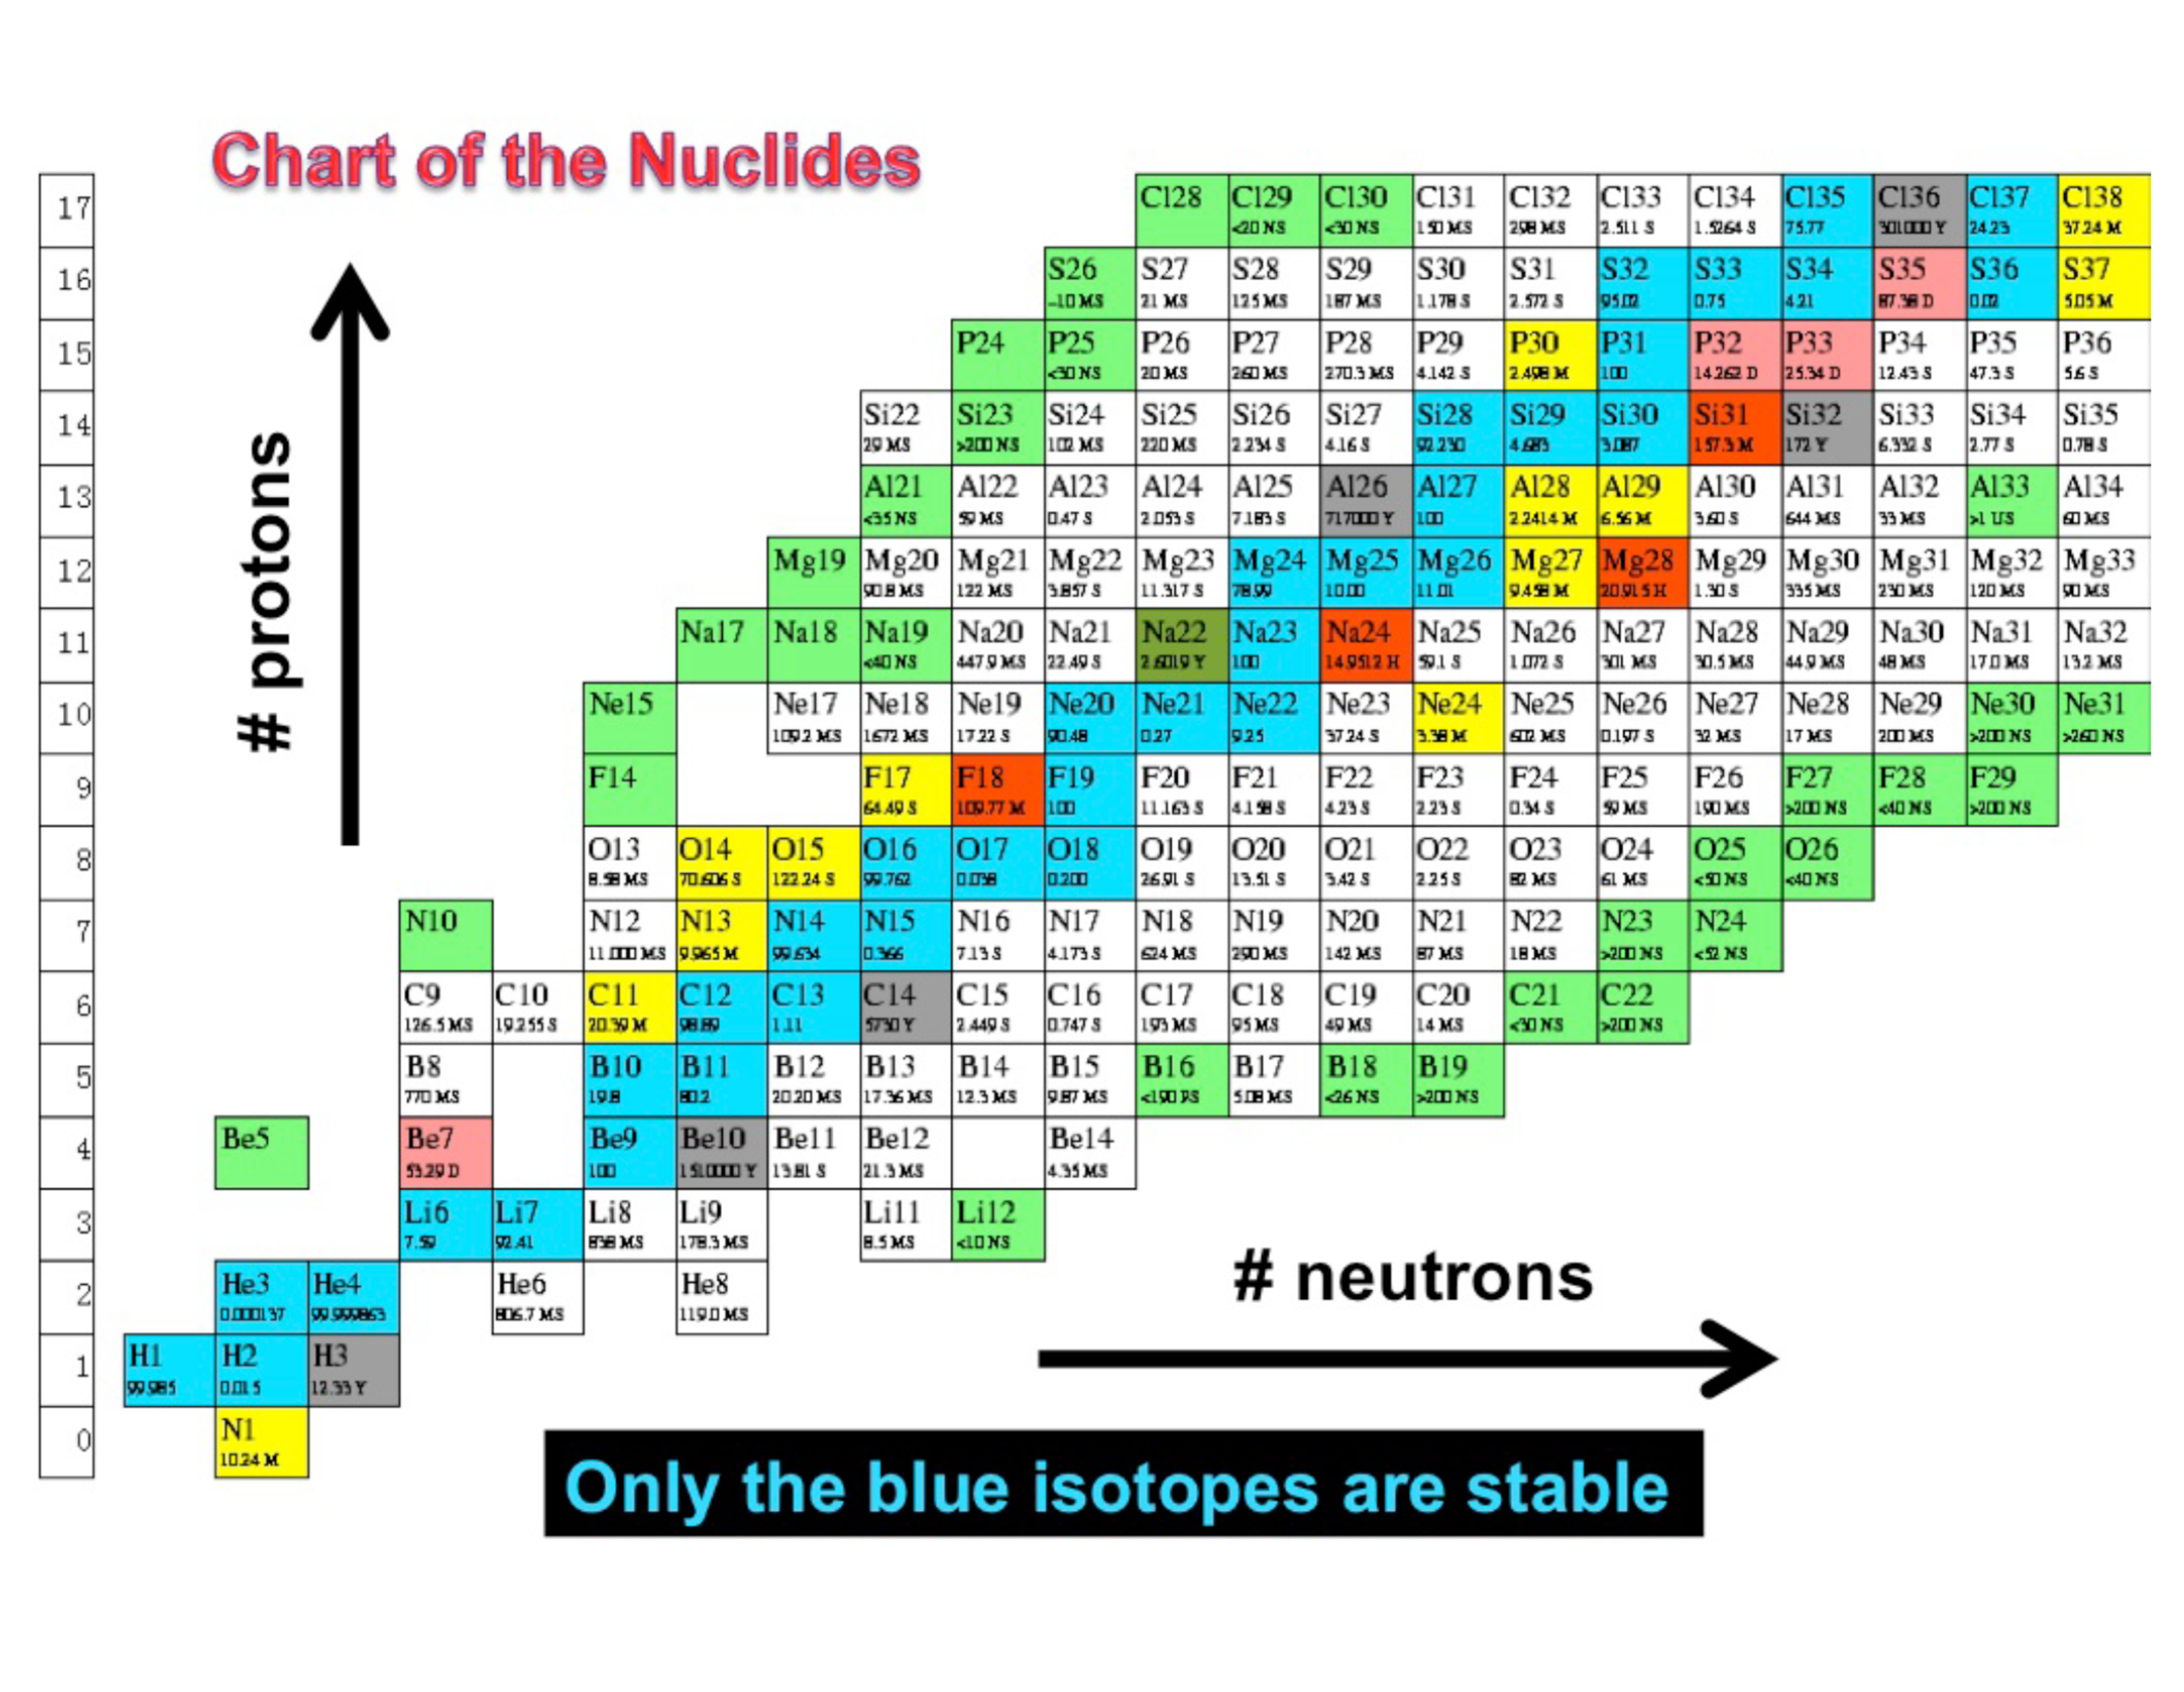
\includegraphics[width=8cm]{lezione 28 novembre/cartaelementistabili.png}
    \label{lezione 28 novembre/cartaelementistabili.png}
\end{figure}

Comunque, sembra che in questo momento questa spiegazione funzioni e che sia possibile prevedere i rapporti osservati delle abbondanze chimiche dei vari elementi più pesanti del ferro. Poiché funziona per tutti simultaneamente, è una teoria consistente. Siamo dunque abbastanza confidenti del fatto che gli elementi più pesanti si siano formati per cattura neutronica. Gli elementi relativamente più leggeri si formano nelle stelle di grande massa, dove si ha il bruciamento dell'elio in carbonio, ossigeno e così via; nelle stelle di grandissima massa possiamo produrre fino al ferro; oltre questo possiamo, per esempio, produrre fino al bismuto nelle AGB, perché prevedono una certa produzione di neutroni; per quanto riguarda invece gli elementi più pesanti non abbiamo una spiegazione. Quindi nelle stelle riusciamo a produrre sicuramente fino al bismuto senza nessuna difficoltà. Questa sembrerebbe essere la tavola periodica così come si dovrebbe essere formato ogni singolo elemento in ogni parte dell'universo.

\begin{figure}[H]
    \centering
    \includegraphics[width=12cm]{lezione 28 novembre/tavolaperiodica.jpg}
    %\caption{Elementi della tavola periodica con relativa origine cosmica}
    \label{lezione 28 novembre/tavolaperiodica.jpg}
\end{figure}

\subsection{Morte delle stelle di piccola massa}
\subsubsection{Nane bianche}
Siamo negli stadi finali di una stella, dopodiché non c'è più una struttura di tipo stellare, ma qualcosa di diverso. Ancora una volta tutto quello che succede dipende dalla massa della stella. Quando si parla di massa della stella, si parla sempre di massa della stella com'era in sequenza principale, quindi per esempio non si tiene conto del fatto che abbia perso parte della sua massa espellendola per dare origine a una nebulosa planetaria. Abbiamo definito la stella centrale "rimanente" come Nana Bianca. Questa nana bianca è un oggetto in cui non ci sono reazioni nucleari, in quanto possiede un core di carbonio che, infatti, non brucia. Brucerebbe solo per stelle da 8 masse solari in su, per cui fino a una stella come il Sole questo oggetto è sicuramente fatto di carbonio. Non può bruciare, non ha una massa sufficiente per raggiungere la temperatura di bruciamento del carbonio. A questo punto la struttura stellare viene sostenuta dalla pressione degli elettroni degeneri. Quindi, se si facesse una sostituzione nell'equazione di equilibrio idrostatico:

$$-\frac{dP}{dr}=\frac{GM\rho}{r^{2}} \rightarrow P \simeq \frac{GM^{2}}{R^{4}}$$

A questa possiamo associare le pressione degli elettroni degeneri:

$$P\simeq \frac{(3\pi^{2}\hbar)^{\frac{2}{3}}n^{\frac{5}{3}}}{5m_e} \simeq \frac{\hbar^{\frac{2}{3}}}{m_e} \left( \frac{M}{R^{3}m_i} \right)^{\frac{5}{3}}$$

Combinando le due espressioni, ricaviamo un'espressione per il raggio e per la densità di queste nane bianche:

$$R \simeq \frac{\hbar^{\frac{2}{3}}}{Gm_{e}m_{i}^{\frac{5}{3}}} M^{-\frac{1}{3}} \simeq 10^{4} \, \text{km} \rightarrow \rho \simeq \rm \frac{10^3 \, kg}{cm^{3}}$$

Quindi questa nana bianca sarebbe un oggetto molto piccolo.

All'inizio questi oggetti sono stati frutto di grande interesse, perché bisognava dimostrare che esistessero. Vedere oggetti come questi non è banalissimo. Essi occupano la regione in basso del diagramma H-R, che è la regione di bassa luminosità.

\begin{figure}[H]
    \centering
    \includegraphics[width=10cm]{lezione 28 novembre/nanebianche.png}
    %\caption{Zona occupata dalle nane bianche nel diagramma H-R}
    %\label{lezione 28 novembre/nanebianche.png}
\end{figure}

Tali stelle sono le più brillanti. Sono inoltre contraddistinte da temperature molto alte all'inizio, poi vanno raffreddandosi, per cui migrano lungo il cammino mostrato in figura. La temperatura va dai 20 mila gradi (stelle di tipo B0), fino a raggiungere temperature più basse di quelle del Sole. Vederle è fattibile, ma bisogna trovarle. Per esempio, osservando Sirio abbiamo scoperto che esso ha una variazione periodica della velocità radiale, per cui Sirio appartiene a un sistema binario.

\begin{figure}[H]
    \centering
    \includegraphics[width=8cm]{lezione 28 novembre/siriob.jpg}
    \label{lezione 28 novembre/nanebianche.png}
\end{figure}

(In figura: Sistema binario formato da Sirio-A e Sirio-B. La seconda è una nana bianca.)

La massa dell'oggetto che girava attorno a Sirio non era facilmente visibile, perché si trattava di una nana bianca. Si vedeva Sirio ruotare attorno a qualcosa che aveva una massa importante, ma che non era visibile, quindi doveva avere un raggio molto piccolo.

(Nota: per convenzione nei sistemi binari l'oggetto più brillante viene identificato dalla lettera A, l'altro dalla lettera B.)

Le nane bianche sono state scoperte osservando le anomalie nel comportamento della velocità radiale di oggetti brillanti che venivano studiati per altri motivi. Per quanto riguarda le nane bianche, se si fa una stima del tempo di raffreddamento, si scopre che durano circa qualche migliaio di anni. Questi oggetti collassano e riducono il proprio raggio, così il periodo di oscillazione diventa più breve. Si può dimostrare che se effettivamente si riduce un Sole al diametro di 10 mila km, il suo periodo di rotazione diventa dell'ordine delle ore. Misurare la velocità di rotazione delle nane bianche è stata una prova effettiva della loro struttura: non erano solo stelle piccole, ma erano stelle piccole e con velocità di rotazione elevate, coincidenti con quelle teoriche; è stata una prova importante. Inoltre le nane bianche presentano un campo magnetico molto grande che nasce dalla condensazione del campo magnetico iniziale, che per il Sole vale circa 1-2 Gauss al polo, quindi diventa, per una stella così compattata, di miliardi di Gauss. Questi campi magnetici si possono misurare e sono consistenti con i valori teorici.

\subsubsection{Supernove di tipo 1}
Le stelle di piccola massa terminano la loro vita come nane bianche. Sono oggetti sostenuti dalla pressione degli elettroni degeneri, cioè la forza gravitazionale dell'oggetto è sostenuta da tale pressione. Questa possibilità esiste se la massa non è più grande di un certo valore. Poiché se la massa aumenta allora anche la forza gravitazionale aumenta, in tal caso sarebbe necessaria una pressione diversa, più alta. Se la massa della nana bianca supera un valore limite, detto \textit{Massa di Chandrasekhar}, la stella collassa indipendentemente dalla pressione degli elettroni degeneri.

$$M_{\rm Chandrasekhar} \simeq \left( \frac{\hbar c}{G} \right)^{\frac{3}{2}} m_{i}^{-2} \simeq 1.44 M_{\odot}$$

Si può ricavare il valore limite della massa di Chandrasekar partendo, come prima, dall'equazione dell'equilibrio idrostatico e dal valore di pressione degli elettroni degeneri, stavolta in campo relativistico per via dell'aumento di densità.(guarda Unsold)

A questo punto cosa accade se una stella con massa pari al valore limite, con nucleo di carbonio, collassa? Lo abbiamo già visto parlando del flash dell'elio. Per l'helium flash, quando abbiamo il collasso, possiamo raggiungere una temperatura sufficiente per bruciare l'elemento successivo. Se si ha una stella superiore a 1.44 $M_{\odot}$, che sarebbe il valore della massa limite di Chandrasekhar, la stella collassa. I dettagli del collasso dipendono, inoltre, dal moto di rotazione della stella e dalla composizione chimica oltre al carbonio. Per masse superiori a Chandrasekar, se le stelle collassano, la loro fase finale non sarà la trasformazione in una nana nera, ma sarà il raggiungimento di una fase esplosiva, in cui il carbonio inizia a bruciare contemporaneamente in tutto il core. Questo processo non è sopportato dalla stella, che ha espulso tutto ciò che non era carbonio, e produce un'esplosione. Stiamo tuttavia parlando di un valore di massa limite di 1.44 $M_{\odot}$, valore molto difficile da raggiungere per una stella di piccola massa (infatti quasi sempre non viene raggiunto da queste stelle). Se la stella ha una massa superiore, ha un'esplosione di tipo supernova, espelle gli strati, ecc.

Esiste la possibilità però anche per le stelle con massa inferiore a 1.44 di esplodere. \E il caso in cui questa stella (di massa inferiore a 1.44 $M_{\odot}$) appartenga a un sistema binario. Infatti, in un sistema binario può accadere che una stella sia più massiva dell'altra.

\begin{figure}[H]
    \centering
    \includegraphics[width=8cm]{lezione 28 novembre/sistemabinario1.png}
    %\caption{Sistema binario formato da una stella più massiva e da una meno massiva.}
    %\label{lezione 28 novembre/sistemabinario1.png}
\end{figure}

Quella più massiva evolverà più rapidamente, per cui raggiungerà prima dell'altra la condizione di nana bianca. Immaginiamo una stella sotto alle 8 masse solari, che si evolve in circa 800 milioni di anni: se avesse una stella come il Sole attorno, che impiega invece 10 miliardi di anni, la prima diventerà una nana bianca, mentre la stella farà la sua vita, evolverà: diventerà una gigante e si espanderà. Espandendosi può trasferire massa alla stella accanto:

\begin{figure}[H]
    \centering
    \includegraphics[width=7cm]{lezione 28 novembre/discoaccrescimento.png}
    %\caption{Trasferimento di massa dalla stella massiva alla nana bianca attraverso il disco di accrescimento.}
    %\label{lezione 28 novembre/discoaccrescimento.png}
\end{figure}

\textbf{approfondisci}Questa situazione si può vedere, perché esistono sistemi binari in cui non riusciamo a vedere gli oggetti però vediamo lo spettro di una stella gigante, lo spettro di un'altra stella che sta orbitando (quindi le velocità radiali) e lo spettro di un disco (che a breve chiameremo disco di accrescimento), perché le righe spettrali prodotte da un oggetto in rotazione hanno una forma particolare, quindi possiamo vedere lo spettro di una stella gigante e lo spettro di una stella che ha un disco. Lo spostamento di massa da un oggetto all'altro non avviene infatti in maniera diretta, ma avviene attraverso la creazione di un disco di accrescimento. Dopodiché la materia si sposta dal disco di accrescimento all'oggetto centrale. Tutto questo lo possiamo vedere con la spettroscopia, non possiamo averne un'immagine. Un po' alla volta si può trasferire massa da un oggetto all'altro, facendogli superare il valore di massa critica.

\begin{figure}[H]
        \centering
        \includegraphics[width=5cm]{lezione 28 novembre/trasferimentomassa.png}
        \label{lezione 28 novembre/trasferimentomassa.png}
    \end{figure}

Nell'esempio in figura, alla nana bianca viene trasferita massa, così supererà il valore limite ed esploderà come Supernova di tipo 1.

Consideriamo ad esempio il Sole. Esso evolverà, e per superare la massa limite gli occorrerebbe mezza massa solare (per raggiungere le 1.44 masse solari). Per raggiungere tale valore dovrebbe avere una compagna, che non ha, per cui il Sole è destinato a raffreddarsi e spegnersi. Se il Sole avesse una stella accanto e questa gli trasferisse la massa mancante per raggiungere le 1.44 masse solari, allora il Sole avrebbe un'accensione del carbonio (in questo core degenere), quindi un insieme di reazioni nucleari che coinvolgono l'intera struttura. In quel momento il Sole esploderebbe.

Questo fenomeno avviene per tutte le stelle allo stesso modo. Si ha una stella sotto le 1.44 masse solari che ad un certo istante arriva al valore limite di 1.44 ed in quel momento esplode. Tutti questi collassi avvengono allo stesso modo e producono tutti la stessa quantità di energia. Per cui tutte le stelle di piccola massa che percorrono questo iter, appartengono a sistemi binari. La secondaria riversa massa, aumentando la massa della primaria fino al valore critico. Si ha un'esplosione con rilascio di energia uguale per tutti gli oggetti, con una magnitudine assoluta pari a $-19.5$ (numero uguale per tutti). Questa luminosità viene raggiunta ad un certo istante, che viene detto tempo zero della supernova.

\begin{figure}[H]
    \centering
    \includegraphics[width=8cm]{lezione 28 novembre/supernovatipouno1.png}
    \label{lezione 28 novembre/supernovatipouno1.png}
\end{figure}

(In figura: Evoluzione temporale della luminosità di una supernova di tipo 1)

In realtà un aumento di luminosità avviene nei 20 giorni precedenti, dopodiché si raggiunge il picco di $-19.5$.

Quello che succede ad una Supernova di tipo 1 è che nel tempo diminuisce la sua luminosità. Il modo in cui la luminosità della stella decresce, permette di distinguerla da altri tipi di supernove. Le supernove di tipo 1 durante la loro evoluzione mostrano spettri sempre diversi, perché man mano si formano elementi chimici diversi, quindi la struttura cambia completamente.

\begin{figure}[H]
    \centering
    \includegraphics[width=8cm]{lezione 28 novembre/spettrisupernova.png}
    \label{lezione 28 novembre/spettrisupernova.png}
\end{figure}

(In figura: Spettri di una supernova di tipo 1. Notiamo come variano totalmente col passare del tempo.)

Quello che caratterizza queste supernove è la totale mancanza di idrogeno in superficie. Siccome non ce n'è, non si vedono le righe dell'idrogeno.

\subsubsection{Supernova nella Nube di Magellano}
La storia delle supernove è stata riscritta il 23 febbraio 1987, data in cui nella grande nube di Magellano, visibile dall'emisfero sud, è stato scoperto qualcosa di nuovo.

\begin{figure}[H]
    \centering
    \includegraphics[width=8cm]{lezione 28 novembre/nubidimagellano.png}
    %\caption{A sinistra della Via Lattea, possiamo vedere le due nubi di Magellano.}
    \label{lezione 28 novembre/nubidimagellano.png}
\end{figure}

Le due nubi di Magellano sono due galassie che ruotano attorno alla nostra. Il 23 febbraio 1987, il puntino indicato nella figura sotto è diventato più brillante di tutto ciò che c'era attorno, e questa è stata l'esplosione della Supernova. L'effetto è stata una variazione non soltanto di luminosità, ma anche morfologica.

\begin{figure}[H]
    \centering
    \includegraphics[width=10cm]{lezione 28 novembre/sn1897a.png}
    \label{lezione 28 novembre/sn1897a.png}
\end{figure}

(In figura: In alto, la Nube di Magellano come appariva il 22 febbraio. In basso a sinistra, come è apparsa il 23 febbraio 1987. In basso a destra, lo stesso oggetto oggi.)

Si ha un'espulsione di strati, quindi la creazione di materia circumstellare, e poi getti di materia, che probabilmente seguono linee di campo magnetico.

\begin{figure}[H]
    \centering
    \includegraphics[width=12cm]{discosupernova.png}
    \caption{Spettro di emissione della Supernova SN1987A, come appare oggi.}
    \label{discosupernova.png}
\end{figure}

Esercizio: nell'emissione radio di una supernova si vede un disco. Quest'esplosione è avvenuta in una stella distante 168 mila anni luce. Potremmo calcolare il diametro di questo oggetto. Quanto misura l'anello che circonda SN1987A? Possiamo calcolarlo. Ciò è una conseguenza del fatto che questa supernova ha una magnitudine intrinseca assoluta pari a -19.5.

\textbf{SISTEMALA STA PARTE AL MASSIMO TOGLILA}

Conoscere la luminosità di un oggetto alla sua superficie, permette di usarlo come un misuratore di distanze. Dato che la sua magnitudine apparente dipende dalla magnitudine intrinseca:

$$m-M=-2.5 \log \frac{L_{obs}}{L}$$
$$m - M = 5 \log d +25$$

Con $m$ magnitudine apparente; $M$ magnitudine assoluta: $L_{obs}$: luminosità osservata; $L$ Luminosità intrinseca; $d$ misurata in megaparsec.

%In caso, aggiustate questa formula se avete già studiato luminosità, magnitudine apparente, ecc ecc DIOPORCO

In ogni caso lui sta parlando di questo:

\begin{figure}[H]
    \centering
    \includegraphics[width=6cm]{lezione 28 novembre/misuradistanze.png}
    \caption{Misurare distanze attraverso valore di magnitudine intrinseca.}
    \label{lezione 28 novembre/misuradistanze.png}
\end{figure}

Conoscere questo e fare una misura restituisce la distanza degli oggetti.

Adesso, l'esistenza di un marcatore di distanze, come le supernove di tipo 1A, è stato fondamentale per dare dimensione all'universo. \E la cosa più accurata che abbiamo.

\vspace{0.2cm}Domanda: la luminosità intrinseca è stimata?

L'astrofisica funziona per passaggi da scale piccole a scale grandi. Fondamentali sono le distanze, dobbiamo conoscerle. Ci sono distanze che possiamo conoscere in maniera immediata. Esempio: la distanza delle stelle dalla Terra con la parallasse trigonometrica. Ci sono inoltre degli oggetti per cui la luminosità dipende solo dalla distanza, e quindi la loro luminosità intrinseca è nota. Esistono le Cefeidi, per esempio, che hanno una luminosità che varia nel tempo periodicamente. Il valore medio della luminosità dipende dal periodo di oscillazione. Scoperta questa classe di stelle, possiamo misurare la distanza di oggetti più lontani. Conoscendo la luminosità intrinseca, possiamo valutare il valore apparente, e quindi la distanza. Si possono attribuire distanze alle stelle a partire da oggetti più vicini.

Abbiamo per esempio un oggetto (supernova di tipo 1) che è esploso all'interno di una galassia (galassia di cui ho misurato la distanza grazie alle Cefeidi). Per cui conosciamo la distanza. Conosciamo quindi la magnitudine apparente, ed anche la magnitudine intrinseca. La teoria vuole infatti che abbiano tutte la stessa luminosità e le osservazioni hanno dimostrato che è vero.

\subsubsection{Supernove come indicatori di distanze}
Dal valore intrinseco di -19.5 delle supernove di tipo 1, che esplodono e decadono con un tipo di curva molto specifico, si possono misurare le distanza delle galassie. Riusciamo a misurare la distanza di galassie lontanissime. Il motivo è che quando esplodono, le supernove di tipo 1 sono luminose quanto le galassie a cui appartengono.

Queste supernove potrebbero essere però il prodotto del superamento della massa critica non per accrescimento lento, ma per "merging" di due oggetti: due stelle sotto la massa critica per qualche motivo collassano. Questo non c'entra niente. Non si tratta di una supernova di tipo 1. Questo è un fenomeno che esiste, ma che non ha una luminosità intrinseca, per cui quando abbiamo supernove che non seguono le regole, si immagina che siano conseguenza dalla coalescenza di più oggetti.

Riassumiamo col seguente grafico l'iter di post-sequenza principale delle stelle di piccola massa:

\begin{figure}[H]
    \centering
    \includegraphics[width=6cm]{lezione 28 novembre/mortestellepiccolamassa.jpg}
    \label{lezione 28 novembre/mortestellepiccolamassa.jpg}
\end{figure}

\subsection{Morte delle stelle di grande massa}
Abbiamo parlato delle fasi finali di un oggetto di piccola massa, cioè minore di 8 masse solari, per cui il carbonio non brucia. Questo oggetto dà vita a una nana bianca. Se la nana bianca ha una massa superiore a quella critica di Chandrasekhar può collassare, altrimenti rimane lì. Può però collassare anche se in un sistema binario riceve massa dalla compagna, quindi si ha una fase esplosiva.

Per quanto riguarda gli oggetti di grande massa, terminato il sostento della struttura per effetto delle reazioni nucleari, si ha il collasso, che non può essere impedito da niente: in questo momento le forze gravitazionali predominano su tutto e la temperatura sale enormemente. Si può avere anche una fotodisintegrazione dei nuclei all'interno. Può avvenire la produzione di neutroni.

Tutti questi processi non fanno altro che sottrarre energia al sistema, che quindi collasserà molto più rapidamente. Se prima c'era una temperatura nelle stelle che, in qualche modo, dava vita a una certa "pressione", questi processi raffreddano il sistema, per cui la pressione associata cala.

La quantità di energia gravitazionale che si potrebbe generare da tutto il sistema che collassa, per una stella di questo ordine di grandezza, è dell'ordine di $10^{53}$. La supernova di tipo 1 sviluppava energia di ordine $10^{51}$, dunque l'energia di collasso di queste stelle è superiore a quella di una supernova.

Che cosa può accadere a questo sistema? Abbiamo una stella che collassa: la parte più densa è all'interno; la massa è superiore al valore critico $M_{\rm Ch}$. All'interno si può venire a creare un core di neutroni, cioè la densità è così alta infatti che protoni e elettroni danno origine a neutroni. Se questo accade, cioè se siamo nelle condizioni tali da ottenere una struttura fatta all'interno di soli neutroni, la struttura totale smette di collassare, poiché la pressione dei neutroni degeneri sostiene tutto. Contro questo core, che di colpo diventa rigido, sta continuando a cadere materia, che si trova quindi a "rimbalzare" su esso: la materia inverte il verso della propria velocità negli strati in cui entra a contatto con questo core. Si sviluppa un'onda di caduta riflessa che incontra gli strati che stanno arrivando. Le velocità relative sono molto alte, per cui si crea un aumento di temperatura degli strati che collassano e si genera una supernova di tipo 2.

\subsubsection{Supernove di tipo 2}
In questo caso le stelle esplodono. Si parla di esplosione quando si ottengono velocità superiori alle velocità di fuga dell'oggetto. Le supernove di tipo 2 sono diverse da quelle di tipo 1 nella curva di luce, cioè nella variazione della luminosità nel tempo.

\begin{figure}[H]
    \centering
    \includegraphics[width=10cm]{lezione 28 novembre/supernovatipouno.png}
    \label{lezione 28 novembre/supernovatipouno.png}
\end{figure}

La curva di luce delle supernove di tipo 2 è dominata non tanto da fotoni creati da un corpo nero che si espande e raffredda, ma contribuisce in maniera sostanziale alla forma della curva di luce la generazione di energia data dal decadimento di nuclei più leggeri.

La caratteristica fondamentale che distingue i tipi di supernove è il fatto che la supernova di tipo 2 viene da un oggetto che all'esterno non ha espulso materia, quindi contiene ancora idrogeno, che appare evidente nello spettro.

\begin{figure}[H]
    \centering
    \includegraphics[width=12cm]{immagini/confronto_spettri_superanova_1_e_2.png}
\end{figure}

(In figura: Confronto degli spettri di emissione dei due tipi di supernove. Notiamo come il secondo sia dominato dall'idrogeno.)

Questo grafico contiene un'informazione data dalla riga dell'idrogeno-$\alpha$: essa ha una porzione di emissione (la parte rivolta verso l'alto) e una porzione in assorbimento (la parte rivola verso il basso). Questa riga ci permette di studiare bene le geometrie dell'oggetto che esplode. Avere una riga in emissione con questa forma, permette di studiare la velocità di espansione. Questa forma caratteristica dei profili delle righe, definita p-cygni (dal prototipo di stella che contiene questo oggetto), permette di determinare la velocità del vento (inteso quello che trasporta il materiale). Di queste supernove possiamo avere il dettaglio di come la stella si sta espandendo.

Queste stelle, a differenze delle altre, non hanno una luminosità intrinseca a priori. Possono essere usate per stimare distanze, ma non appartengono alla categoria degli indicatori di distanze. Sono oggetti molto particolari, perché in queste sembra che si possano formare gli elementi pesanti che mancavano prima.

In una supernova di tipo 2 quello che accade è che gli strati più esterni che sono espulsi danno origine a strutture, dette resti della supernova, che hanno forme di tipi molto diversi dalle nebulose.

\begin{figure}[H]
    \centering
    \includegraphics[width=8cm]{lezione 28 novembre/supernovarem1.png}
    %\caption{Supernova Remnants}
    \label{lezione 28 novembre/supernovarem1.png}
\end{figure}

All'interno dei resti della supernova sta l'oggetto responsabile dell'esplosione, che non è sempre visibile, per poca luminosità e piccole dimensioni.

\subsubsection{Raggi cosmici}
Le esplosioni delle supernove hanno un ulteriore ruolo nella chimica dell'universo oltre all'espulsione di materia processata, quindi elementi pesanti che vengono rimessi nel circolo, per dare eventualmente vita a nuove stelle.

In queste regioni, che sono caratterizzate da questi filamenti (vedi immagine sopra), si possono avere dei campi di velocità molto alti. Sono regioni caratterizzate dalla presenza di campi magnetici. In queste regioni elettroni e protoni si muovono molto velocemente, in più c'è un campo magnetico, per cui si possono ottenere ulteriori accelerazioni delle particelle per effetto dell'accelerazione di Fermi. Le particelle possono essere molto accelerate e dare origine ai raggi cosmici.

Sulla Terra arrivano una certa quantità di nuclei, di composizione chimica simile a quella del Sole, con numerosità che dipende dalla loro energia. Questi raggi cosmici che vediamo sulla Terra, si pensa siano prodotti dai resti delle supernove. I raggi cosmici sono importanti perché permettono di studiare la cinematica e tutto quello che succede all'interno della supernova; ad esempio si cerca di capire come la materia venga espulsa dalle supernove, o come si vengano a formare. Essi sono responsabili di un'ulteriore modifica della chimica del cosmo. Infatti possono creare elementi per spallazione\footnote{Processo fisico tramite il quale un nucleo pesante emette una grande quantità di nuclei più leggeri a seguito di collisione con una particella ad alta energia.}; questo fa sì che ci siano alcuni elementi, su tutti berillio e boro, che sono una conseguenza diretta dei raggi cosmici.
\subsubsection{Popolazioni stellari}

Tutta questa variazione della chimica del cosmo porta alla definizione attuale di due popolazioni stellari. Cioè, se in questo momento facciamo spettri di una stella, troviamo spettri come questi:

\begin{figure}[H]
    \centering
    \includegraphics[width=12cm]{lezione 28 novembre/popolazionistellari1.png}
    \label{lezione 28 novembre/popolazionistellari1.png}
\end{figure}

(In figura: Spettri di emissione di una stella di popolazione 2 (in basso) ed una di popolazione 1 (in alto).)

Vediamo nello spettro (A) intense righe dell'idrogeno quali H-$\gamma$ e l'H-$\delta$ e pochissime righe in mezzo. Le stelle associate a questo spettro si dicono di popolazione 2. Poi vediamo un'altra classe, detta di popolazione 1, i cui spettri (B) sono pieni soprattutto di righe spettrali di metalli (oltre a quelle di idrogeno). La popolazione 1 è detta di alta metallicità, quella 2 di bassa metallicità.

Si pensa che le stelle di popolazione 1 siano quelle giovani, formate dagli elementi espulsi dalla popolazione precedenti, le old star, dette invece di popolazione 2. Se osserviamo lo spettro di queste stelle, quello che vediamo è che cambia il contenuto dei metalli.

\begin{figure}[H]
    \centering
    \includegraphics[width=12cm]{lezione 28 novembre/bassametallicita.png}
    \label{lezione 28 novembre/bassametallicita.png}
\end{figure}

(In figura: Spettri di emissione di varie stelle. In blu di una stella a bassa metallicità; in verde e rosso di stelle ad alta metallicità.)

In alto a destra del grafico troviamo la nomenclatura usata per indicare l'abbondanza di un elemento rispetto all'idrogeno. Le tra parentesi quadre indica che tale abbondanze sono calcolate per il sole.

Gli spettri diventano sempre più poveri di righe perché non ci sono metalli. Quindi i fotoni prodotti nella stella vengono fuori in modo diverso. Il motivo è che se non ci sono metalli, come nello spettro blu in figura, sostanzialmente, i fotoni ultravioletti possono uscire. In una stella con più metalli come quella rossa, i fotoni vengono bloccati, il che non significa che vengono distrutti, ma che vengono emessi con un'altra lunghezza d'onda. Quindi viene emesso un altro spettro, che presenta più flusso nell'infrarosso. L'area di queste tre curve è uguale. La differenza tra gli spettri di emissione verde e rosso è quello che interpretiamo come un diverso contenuto di metalli. Alle popolazioni 1 e 2 dovremmo associare una presunta popolazione 3, che non è mai stata osservata, e che includerebbe, virtualmente, gli spettri senza metalli.

\subsubsection{Stelle di neutroni}
Abbiamo visto il risultato dell'evoluzione stellare e di come questo possa cambiare la chimica dell'universo, cioè della generazione successiva. Resta da risolvere un altro problema: che cosa è successo nei nuclei di queste supernove, che neppure vediamo?

La stella di neutroni che si è venuta a formare, che conteneva tutto, si comporta in maniera diversa a seconda della sua massa. Definiamo anche una massa critica, detta \textit{massa di Oppenheimer-Volkoff}, che è compresa tra le due e le tre masse solari. Allora, può accadere che questo oggetto di neutroni resti stabile, quando ha una massa inferiore a 2 o 3 masse solari. Avremo una stella fredda, fatta di soli neutroni. Questi oggetti sono molto compatti. Possiamo calcolarne il raggio, usando la pressione dei neutroni degeneri e combinandola con l'equazione di equilibrio, similmente a come abbiamo fatto per le nane bianche. Dai calcoli si ottiene che il raggio è di circa 10 km. Una stella di neutroni è quindi un oggetto molto piccolo e denso: meno di 2/3 masse solari, in una sfera di raggio 10 km. Hanno una velocità di rotazione elevata: girano 600 volte al secondo. Possiede inoltre un campo magnetico estremamente alto.

Non le possiamo vedere: gli oggetti al centro dei resti di una supernova non sono visibili, non hanno un'emissività sufficiente. La ragione è che al di là della loro temperatura, il loro raggio è talmente piccolo da renderli invisibili. Possiamo in realtà vederle guardando non alla loro emissione ottica ma all'emissione radio. Negli anni '60 furono scoperti alcuni oggetti, noti come \textit{pulsar}, oggetti che presentavano, nel radio, delle emissioni periodiche. Il tempo tra un'emissione e l'altra è molto breve, molto inferiore al secondo.

\begin{figure}[H]
    \centering
    \includegraphics[width=12cm]{lezione 28 novembre/emissione periodica.png}
    \label{lezione 28 novembre/emissione periodica.png}
\end{figure}

(In figura: Emissione periodica registrata da una pulsar.)

L'interpretazione data ai pulsar, che si trovano nei centri dei resti di supernove (la più famosa è la Crab, che presenta un'emissione periodica, con periodo di 33 millisecondi), è che queste sono nient'altro che il risultato del collasso. La stella di neutroni gira su se stessa e presenta un campo magnetico molto intenso, per cui gli elettroni sono costretti a co-ruotare con il campo magnetico, che gira con periodo di 33 millisecondi. Questi elettroni che ruotano emettono radiazione (poiché le cariche accelerate producono un emissione di sincrotrone) e tutte le volte che questo campo magnetico, che è inclinato rispetto all'asse di rotazione, punta verso di noi, vediamo l'impulso radio.

Le pulsar, la cui spiegazione qualitativa è stata data da Franco Pacini, nel 1967, sono considerate la prova che tutto ciò che abbiamo studiato finora terminava, per le stelle di grande massa, con le stelle di neutroni.

\subsubsection{Buchi neri}
Se invece il nucleo della stella di neutroni ha una massa superiore al valore critico di Oppenheimer-Volkoff, neanche la pressione dei neutroni degeneri può sostenere la struttura, che continuerà a collassare. Se questo oggetto esistesse, darebbe origine a qualcosa che non vediamo in quanto la massa limite di questo oggetto non è quantificabile: se il collasso continuasse all'infinito, senza essere compensato da alcuna forza, otterremo un raggio molto piccolo, molto più piccolo di quello che dovrebbe essere il valore minimo per permettere alla luce di uscire (raggio di Schwartzschild). Ricordiamo che questo è il raggio di una massa la cui velocità di fuga è superiore a quella della luce:

$$R_{\rm Sch}=\frac{2GM}{c^2}$$

Se questo fosse vero, avremmo oggetti di cui non vediamo la superficie, poiché questo raggio diventerebbe una specie di "orizzonte". Non è importante quanto sia grande, ma il fatto che non sia visibile. Questo oggetto non ha più emissione. Nell'immaginario collettivo questo oggetto si chiama \textit{buco nero}.

Dei buchi neri non si sa niente di certo in quanto non ci sono evidenze dirette. Quello che sappiamo è che ci possono essere evidenze indirette della loro esistenza. Per esempio, se in un sistema binario l'oggetto al centro dovesse diventare un buco nero, ci aspetteremmo che il disco di accrescimento sia quasi pieno, cioè che non abbia più la parte centrale.

\begin{figure}[H]
    \centering
    \includegraphics[width=8cm]{lezione 28 novembre/discobuconero.png}
    \label{lezione 28 novembre/discobuconero.png}
\end{figure}

(In figura: Sistema binario, con disco di accrescimento attorno al Buco Nero.)

Con questo genere di calcolo si possono fare previsioni. Data la velocità di rotazione del disco, si può stimare come la materia "cadrebbe" sul buco nero, che quindi aumenterebbe ancora la sua massa. Questo porterebbe a vedere le regioni più interne delle stelle come regioni che emettono radiazione X. Questo è fattibile.

Immaginiamo adesso un'emissione spettrale, una riga spettrale, di un atomo che si trovi in questo campo gravitazionale. Gli orbitali avrebbero delle forme molto particolari, molto diverse per via del "tempo". Il tempo inizia a scorrere in modo diverso, i tempi di decadimento cambiano totalmente e profili di queste righe non hanno niente a che fare con i profili visti finora. Queste cose si osservano, quindi abbiamo un'evidenza indiretta. Abbiamo forti evidenze della realtà di questi oggetti, per esempio l'emissione X.

Quanto detto è il caso di una stella che diventa un buco nero. Esiste anche la possibilità che la massa di Oppenheimer sia superata per coalescenza (fusione) di più masse, il che genera confusione (basta immaginare il centro di una galassia e a quanti oggetti e stelle stanno orbitando, e quindi a quante stelle potrebbero fondersi). Nei centri delle galassie, facendo una stima dalle orbite delle stelle che ruotano attorno al centro galattico, si possono stimare che ci sono buchi neri, non di qualche masse solare, ma di milioni, di miliardi di masse solari. Anche al centro della nostra galassia dovrebbe esserci uno di questi. Questo lo studiamo attentamente dalle orbite di alcune stelle che noi vediamo.

\begin{figure}[H]
    \centering
    \includegraphics[width=6cm]{lezione 28 novembre/centrogalattico.png}
    \label{lezione 28 novembre/centrogalattico.png}
\end{figure}

(In figura: Osservazione di vari corpi celesti che sembrano orbitare attorno al buco nero presente al centro della nostra galassia.)

Al centro della nostra galassia dovrebbe esserci "qualcosa" che ha una massa pari a 4 milioni di masse solari. Non può essere materia ordinaria, che ovviamente avrebbe un volume diverso.

L'ultima evidenza dei buchi neri super massivi, viene fuori dall'esperimento che misura la materia in orbita attorno al buco nero nell'emissione radio. L'umanità ha messo insieme un apparato di radiotelescopi. Abbiamo usato tutto il pianeta per fare questa cosa. Non abbiamo una vera fotografia, ma un'immagine ricostruita per interferometria.

\begin{figure}[H]
    \centering
    \includegraphics[width=12cm]{lezione 28 novembre/immaginericostruita.png}
    \label{lezione 28 novembre/immaginericostruita.png}
\end{figure}

Abbiamo parlato di interferometria, cioè: non abbiamo l'immagine diretta, ma la variazione di luminosità con la distanza (come l'esperimento di Young con le due fenditure) per cui, valutando la variazione di luminosità con la distanza, possiamo ricostruire l'immagine dell'oggetto. L'unica cosa che si vede è un oggetto di forma circolare. Vediamo l'aumento di luminosità. 

\subsubsection{Recap fasi finali delle stelle}
Facciamo adesso una raccolta di ciò che accade alle stelle in funzione della massa iniziale:

\begin{itemize}
    \item Le stelle sotto $1/100 \, M_{\odot}$ non bruciano neanche il deuterio;
    \item Sotto $8/100 \, M_{\odot}$ non bruciano l'idrogeno: nane brune;
    \item Sotto $0.5 \, M_{\odot}$ non si brucia l'elio e si ottiene una nana bianca di elio;
    \item Sotto $1.44 \, M_{\odot}$ avremo una nana bianca di carbonio;
    \item Sotto le $2.25 \, M_{\odot}$ abbiamo le masse caratteristiche dell'helium flash;
    \item Per $2-3 \, M_{\odot}$ abbiamo le stelle di neutroni;
    \item Sotto $8 \, M_{\odot}$ non brucia il carbonio;
\end{itemize}

\begin{figure}[H]
    \centering
    \includegraphics[width=8cm]{lezione 28 novembre/tabellamassefinali.png}
    \label{lezione 28 novembre/tabellamassefinali.png}
\end{figure}

Vediamo infine come masse iniziali possono dare origine a masse negli stati finali.

\begin{figure}[H]
    \centering
    \includegraphics[width=8cm]{lezione 28 novembre/evoluzionemasse.jpg}
    %\caption{Evoluzione stellare nel tempo. Si mette in evidenza la variazione di massa.}
    \label{lezione 28 novembre/evoluzionemasse.jpg}
\end{figure}

Queste stelle all'inizio hanno valori più grandi, ma anche enormi perdite di massa, per cui nell'oggetto finale la massa si riduce. Le stelle di grande massa possono avere una fase analoga a quella di nebulosa planetaria, con una grande espulsione di massa. Come avviene per le Wolf-Rayet.

Le stelle di grandissima massa, sopra 25 masse solari, possono avere una perdita di massa che non è esplosiva. Ce ne sono pochissime di queste. Sono grandissime e molto luminose. Ce ne sono anche nella nostra galassia, ma sono pochissime, in quanto la loro vita media è molto breve. Non è una fase di supernova, non esplodono, perdono solo massa.

\subsection{Nascita delle stelle}
Abbiamo visto le stelle come oggetti auto-gravitanti, che sono in equilibrio perché esiste una forma di produzione di energia, e le abbiamo collocate nel diagramma H-R, fondamentale per ricordare cosa accade alle stelle nel tempo, ossia la loro evoluzione che abbiamo chiamato fase di post-sequenza principale. In realtà, le stelle devono provenire da qualche parte, cioè ci sarà un momento in cui si formano.

L'idea è che le stelle nascano da gas diffuso che appartiene alla galassia. Da che parte cominciare?
\subsubsection{Mezzo interstellare}

\begin{figure}[H]
    \centering
    \includegraphics[width=8cm]{lezione 28 novembre/mezzointerstellare.jpg}
    \label{lezione 28 novembre/mezzointerstellare.jpg}
\end{figure}

Tra le stelle vediamo materia diffusa, gas diffuso. Un'idea è che questo, che è il mezzo interstellare, sia la materia da cui per aggregazione nascano le stelle.

Questi oggetti che visualizziamo sembrano avere grande estensione, ma di cosa sono fatti? Prima di dire che la nube, per aggregazione, dia origine a una stella, bisogna vedere se c'è compatibilità nella composizione chimica. Le nubi interstellari sono fatte della stessa materia delle stelle? Se così non fosse, dovremmo cercare altrove l'origine delle stelle.

Dall'analisi chimica sembra che il mezzo interstellare abbia composizione chimica estremamente compatibile con quella del Sole, cioè è costituito per la maggior parte da idrogeno ed elio. Per queste nubi notiamo anche l'emissione spettroscopica propria di molecole, anche complesse. Allora di cos'altro sono fatte queste nubi?
 
\begin{figure}[H]
    \centering
    \includegraphics[width=10cm]{lezione 28 novembre/composizionenubi.png}
    %\caption{Tipi di ambienti che ritroviamo nel mezzo interstellare.}
    \label{lezione 28 novembre/composizionenubi.png}
\end{figure}

Possiamo avere ambienti con molecole di idrogeno neutro, con pochi atomi ionizzati, a centinaia di kelvin (temperature quindi molto basse), con densità abbastanza elevate (da 1 a 1000 atomi per $\rm cm^3$); altri ambienti con temperature alte, molto rarefatti, con idrogeno ionizzato parzialmente; altri con temperature alte, densità bassissime e idrogeno tutto ionizzato; infine ambienti con temperature molto basse, densità alte e atomi di idrogeno neutri, accompagnati da molecole. Queste sono le quattro possibili categorie del mezzo interstellare.

Che molecole troviamo? Di tutto: troviamo ad esempio molecole diatomiche. Infatti abbiamo prodotto carbonio, ossigeno, troveremo CO; abbiamo zolfo, ferro, azoto, ecc. Nel mezzo interstellare la materia espulsa da stelle di generazione precedente si raffredda e si lega in molecole. Possiamo avere molecole più complicate, come il benzene.

Se misuriamo gli spettri di emissione radio, possiamo osservare anche molecole più vicine alla chimica organica. La presenza di molecole "organiche" lascia ben sperare sull'origine della vita nello spazio, dato che tali molecole esistono a prescindere nello spazio.

Questo mezzo interstellare può essere all'origine di tutte le stelle?

\subsubsection{Collasso delle nubi interstellari}
Perché una nube interstellare collassa?

Ricordiamo il Teorema del Viriale, il quale afferma che l'energia potenziale è pari al doppio dell'energia cinetica.

$$2K + U = 0$$

\rule[7pt]{\linewidth}{0.4pt}

Riportiamo qui, per questioni di completezza e come approfondimento, una semplice dimostrazione del teorema del Viriale presa da \textit{P. Monaco,
"Introduzione all'astrofisica"}, sez. 2.2.

\vspace{0.2cm}Integriamo l'equazione dell'equilibrio idrostatico, dal centro ($c$) alla superficie ($s$) di una stella, moltiplicando prima entrambi i membri per $4 \pi r^3$:

$$\int_{P_c}^{P_s} 4 \pi r^3 \; dP=-\int_{0}^{R} 4 \pi r G M \rho \; dr$$

Nel primo membro riconosciamo $4 \pi r^3=3V(r)$, per semplificare il secondo membro utilizziamo l'equazione di continuità

$$3 \int_{P_c}^{P_s} V \; dP=-\int_{0}^{R} \frac{GM}{r} \; dM$$

Naturalmente il valore di $M$ alla superficie, $M_s$, è uguale al valore della massa della stella.

Riconosciamo subito nel secondo termine l'energia potenziale totale della stella:

$$-\int_{0}^{R} \frac{GM}{r} \; dM=\Omega$$

Il primo termine si può integrare per parti, ottenendo

$$\int_{P_c}^{P_s} V \; dP
=PV\big|_{c}^{s} - \int_{c}^{s} P \; dV$$

Di questi due termini il primo si annulla sia al centro ($V=0$) che alla superficie ($P=0$). Inoltre:

$$3 \int_{c}^{s} P \; dV=2 \int_{c}^{s} \frac{3}{2} nkT=2K \; dV$$

non è altro che 2 volte l'energia cinetica totale delle particelle della stella, ovvero la sua energia
termica. Otteniamo così l'equazione:

$$2K + \Omega=0$$

Questa equazione è nota come teorema del viriale, ed è valida per gas perfetti in equilibrio
idrostatico così come per molti altri casi, come le orbite Kepleriane o il moto delle stelle in
ammassi o galassie.

\textbf{EXTRA:} Questa osservazione sembra interessante ma non so ancora dove metterla.

Un'interessante conseguenza del teorema del viriale è la seguente.

Una nube di gas, che supponiamo in quasi-equilibrio idrostatico\footnote{Per quasi-equilibrio idrostatico intendiamo che il collasso procede con un tempo scala molto più grande del tempo dinamico della nube, cosicché la condizione di equilibrio idrostatico è sempre approssimativamente rispettata.}, collassando si riscalda, e riscaldandosi assume facilmente temperature maggiori di quelle dello spazio esterno, che sono dell'ordine della temperatura del fondo cosmico di radiazione (all'epoca attuale $\sim$2.7 K). Per la seconda legge della termodinamica, la nube irradierà parte della sua energia termica, per raggiungere l'equilibrio termico con l'esterno. Ma questo processo è regolato dal teorema del viriale, per il quale
$2K + \Omega = 0$. Se $E = K + \Omega$ è l'energia totale della nube, allora si ha $E = -K$ oppure $E = \Omega/2$.

Per una nube che irradia, l'energia totale $E$, che è negativa se la nube è gravitazionalmente legata, diminuisce diventando così più negativa. Di conseguenza, l'energia potenziale diminuisce e l'energia termica aumenta! In altre parole, il collasso fa riscaldare la nube, allontanandola ulteriormente dall'equilibrio idrostatico. Quest'apparente violazione del seconda legge della termodinamica è il motivo principale per cui l'universo non è un brodo uniforme di particelle a temperatura molto bassa; tutta l'evoluzione dell'Universo può essere vista come una competizione tra gravità, che tende a creare diversità, e termodinamica, che tende a uniformare.

\rule[7pt]{\linewidth}{0.4pt}

Questa relazione permette di stabilire una condizione di equilibrio della materia: se siamo in una condizione in cui il doppio dell'energia cinetica dei costituenti eguaglia il potenziale gravitazionale, allora il sistema è in equilibrio.

Tale teorema ci dà la possibilità di stabilire alcune condizioni per il mezzo interstellare, così da poter capire se questo possa collassare o meno. Abbiamo detto che la nube ha una composizione chimica compatibile con la formazione delle stelle, ma bisogna capire se la nube può collassare. Partendo dal teorema del Viriale, ci chiediamo qual è la condizione. Leghiamo l'energia cinetica alla temperatura, dato il numero di particelle.

$$K=\frac{3}{2} N k_{B} T$$

Supponiamo che la nube sia una sfera. Sotto questa ipotesi, il potenziale della sfera diventa:

$$U=-\frac{3}{5} \frac{GM^{2}}{R}$$

Queste due relazioni, sostituite nel teorema del Viriale, restituiscono una relazione che lega temperatura, massa e dimensione della nube. All'equilibrio si ha:

$$3Nk_{B}T=\frac{3}{5} \frac{GM^{2}}{R}$$

La nube non collassa e non si espande. Quando collassa? Per:

$$3Nk_{B}T <\frac{3}{5} \frac{GM^{2}}{R}$$

Quando si ottiene questa condizione? Riscriviamo la formula. Supponendo che la densità sia costante, poniamo:

$$N=\frac{M}{m}$$

con $M$ massa della nube e $m$ massa media dei singoli elementi costituenti. Inoltre:

$$\rho = \frac{M}{\frac{4}{3}\pi R^{3}}$$

Da cui ricaviamo un'espressione per R:

$$R=\left( \frac{3M}{4\pi \rho} \right)^{1/3}$$

Sostituiamo l'espressione di $R$ appena trovata nell'equazione sopra e la risolviamo rispetto a $M$:

$$M_{J}=\left( \frac{5k_{B}T}{Gm} \right)^{3/2} \left(\frac{3}{4\pi \rho} \right)^{1/2}$$

Definiamo questo valore di $M$ come \textit{Massa di Jeans}.

Abbiamo espresso la massa della nube in termini delle sue grandezze termodinamiche: temperatura e densità\footnote{Ma la densità è una grandezza termodinamica?????}. All'equilibrio si ha l'uguaglianza. Perché una nube collassi, questa dovrebbe avere massa maggiore di quella di Jeans: $M_{\rm nube}>M_{J}$. In tal caso il potenziale gravitazionale sarà maggiore dell'energia cinetica dei costituenti e si avrà il collasso.

Tra tutte le tipologie di nubi che abbiamo individuato, possiamo indicare quali soddisfano questi criteri, cioè per quali è possibile il collasso.

Esprimiamo la Massa di Jeans in funzione della Massa del Sole:

$$M_{J}=15.4 M_{\odot} \left( \frac{T}{1 \, \text{K}} \right)^{3/2} \mu^{-2} \left( \frac{n}{1 \, \text{cm}^{-3}} \right)^{-1/2}$$

In questo la Massa di Jeans diventa proporzionale alla temperatura e al numero di particelle.

\E l'unico "ingrediente" necessario per determinare il collasso di una nube? Ovviamente solo nel caso più semplice: realisticamente è necessario conoscere se avvengono altri fenomeni, ad esempio sapere se la nube si trovi in rotazione oppure no.

%La condizione sulla massa vale "solo in una direzione" (non ho capito... in che senso?\textbf{chedi a marika}), quindi possiamo avere che una sfera collassi in un disco ma non è detto che il collasso prosegua.

Noi supponiamo che queste nubi siano in rotazione, ma perché dovrebbero esserlo? Si sta conservando un momento angolare? Una nube potrebbe essere in rotazione perché l'intera galassia si trova in rotazione, quindi la rotazione della nube può essere conseguenza della rotazione dell'intera galassia? Non è ben chiaro. Quello che consideriamo vero è che la nube ruoti perché ci serve che ruoti, visto che le stelle ruotano. Abbiamo bisogno che le nubi ruotino, altrimenti non sapremmo spiegare l'origine della rotazione delle stelle. Quindi occorre questo ingrediente, sebbene non c'è nessuna evidenza che queste nubi ruotino.

In base ai valori numerici che conosciamo per le nubi abbiamo tre categorie:

\begin{center}
    \begin{tabular}{llllll}
        & $T$ (K) & $n$ (cm$^3$) & $\mu$ & $M_J \, (M_{\odot})$ & $t_{\rm din}$ (yr)\\
        \hline
        \\[-0.4cm]
        Calde & $10^4$ & $10^{-1}$ & 0.6 & $1.4 \times 10^8$ & $2.3 \times 10^8$\\
        Fredde & $10^2$ & 10 & 1 & $4.9 \times 10^3$ & $1.6 \times 10^7$\\
        Molecolari & 10 & $10^{3}$ & 2 & 3.9 & $1.2 \times 10^6$\\
    \end{tabular}
\end{center}

Il peso molecolare dipende da come la massa si suddivide una molecola nei suoi costituenti, nel caso questi fossero ionizzati; ad esempio se abbiamo idrogeno ionizzato, la massa molecolare diventerà 2. Facendo questa operazione, viene fuori che le uniche nubi che possono collassare sono quelle molecolari, in quanto per queste la massa di Jeans vale soltanto 4 masse solari; tutte le altre darebbero masse troppo grandi per formare una stella. Se prendessimo ad esempio una nube calda, servirebbero 100 milioni di masse solari per farla collassare (d'altra parte non esistono stelle con massa così grande). L'ultimo parametro della tabella è il tempo dinamico di Kelvin-Helmotz, cioè l'equivalente di quello che abbiamo calcolato per il Sole, che collassava in 30 milioni di anni. Quindi, le nubi molecolari sembrerebbero le uniche per cui è possibile il collasso. In effetti esistono nell'Universo tante nubi molecolari, ad esempio i celebri Pilastri della Creazione. L'unico problema è che, per quanto numerose, non bastano, cioè non è possibile immaginare che tutte le stelle finora nate si siano generate dalla condensazione delle sole nubi molecolari; c'è bisogno che collassino altri oggetti, con temperature più alte e densità più basse, ecc.

Questo processo non sempre è immediato, anzi, passa per un lungo stadio intermedio. L'idea che un'intera nube molecolare possa collassare (poiché presenta massa superiore alla massa di Jeans) non funziona, tranne che per pochi casi. Esiste però la possibilità che una grande nube collassi localmente e che quindi si frammenti in una serie di nubi più piccole. Numericamente tale fatto è facile da spiegare: se abbiamo una nube (con moti molecolari turbolenti), è possibile l'aggregazione delle molecole in frammenti con densità più alte, all'interno della nube. Quindi abbiamo dei collassi locali. Questo dà origine alla detta \textit{frammentazione}.

\begin{figure}[H]
    \centering
    \includegraphics[width=10cm]{lezione 28 novembre/frammentazione.png}
    %\caption{Frammentazione: nube che si addensa in frammenti; collassi locali.}
    \label{lezione 28 novembre/frammentazione.png}
\end{figure}

La frammentazione può avvenire anche perché subentra una perturbazione della condizione d'equilibrio della nube. Immaginiamo una nube con all'interno una stella che esplode. L'onda d'urto della stella che esplode potrebbe causare rapidamente la frammentazione e il collasso della nube (che non supera la massa di Jeans).

Persiste ancora il problema di come quella stella sia nata prima per poi dare origine (esplodendo) alla frammentazione. Le stelle non sono mai da sole: stanno nelle galassie. Il Sole ad esempio impiega 220 milioni di anni per fare un giro completo della galassia, potrebbe passare vicino a una nube nel momento in cui esplode. Non è detto però che stella che esplode e nube molecolare si siano formate contestualmente, potrebbero essersi formate indipendentemente, per poi ritrovarsi vicine nel momento fatidico, a causa della trasformazione (movimenti interni) della galassia.

Quindi, come si è formato il Sole? Qua la situazione si complica. Noi abbiamo un Sole che ruota, con un campo magnetico per cui tra i nostri ingredienti (per la formazione stellare) dobbiamo mettere, oltre alla forza centrifuga, anche l'eventuale effetto del campo magnetico. Questo genere di calcolo è ostico, non ci sono soluzioni consolidate su questo aspetto. Sappiamo che questo fenomeno avviene. Sappiamo che le nubi collassano. \E evidente che dove c'è una stella, ne ritroviamo sempre un certo numero, nel senso che le stelle stanno sempre in altri ambienti dove ce ne sono altre: parliamo infatti di \textit{ammassi stellar}i. Queste stelle, che si trovano spazialmente nello stesso luogo, sono caratterizzate da una velocità uguale; se ad esempio dalla Terra osserviamo le Pleiadi, si scopre che tutte le stelle di questo ammasso posseggono tutte la stessa velocità. Tale fatto fa pensare che si siano formate tutte da una stessa nube che aveva una sua velocità, la quale è collassata (frammentandosi prima), in un certo numero di stelle. \E comprensibile quindi il perché abbiano tutte la stessa velocità rispetto alla Terra. L'idea della frammentazione, al di là di dettagli che non sono assolutamente compresi (nel criterio di Jeans, infatti, una situazione del genere non collasserà mai), sappiamo che accade. Il collasso delle nubi molecolari è un aspetto ancora poco chiaro dell'astrofisica. Quello che sappiamo è che, guardando agli ammassi stellari, possiamo calcolare come le stelle si distribuiscono in massa all'inizio.

\begin{figure}[H]
    \centering
    \includegraphics[width=10cm]{lezione 28 novembre/demografiastelle.png}
    %\caption{Distribuzione delle stelle all'interno di un ammasso in base alla massa.}
    \label{lezione 28 novembre/demografiastelle.png}
\end{figure}

Per esempio, prese cento stelle, una sola sarà di grande massa. Le stelle di grande massa quindi non solo evolvono rapidamente, ma sono anche rare. La maggior parte delle stelle in un ammasso sono piccole e durano a lungo.

Queste considerazioni vengono fuori misurando le masse stellari. Cosa accadrebbe se volessimo seguire il collasso di una nube, in quanto fenomeno osservabile? Supponiamo che avvenga il collasso, ci sarebbe una maggiore aggregazione al centro e si creerebbe un core pre-stellare (ancora non è una stella, non è sostenuto dall'idrogeno che brucia).

\begin{figure}[H]
    \centering
    \includegraphics[width=5cm]{lezione 28 novembre/coreprestellare.png}
    %\caption{Core pre-stellare.}
    \label{lezione 28 novembre/coreprestellare.png}
\end{figure}

In questo ambiente che collassa si nota una caratteristica tipica del Teorema del Viriale: l'oggetto collassa, ma solo metà dell'energia potenziale si trasforma in energia cinetica. Ciò avviene perché metà energia potenziale viene persa, espulsa sotto forma di fotoni. Quello che succede è che l'ambiente si riscalda, quindi i fotoni vanno via. Siccome parliamo di molecole, parte dell'energia viene usata per rompere i legami molecolari. L'emissione di bassa temperatura, per nubi a centinaia di kelvin, è ovviamente piccata nell'infrarosso (la nostra Terra ha un picco a 10 micron di emissione di corpo nero e siamo a 300 K. Queste sono ancora più basse, per cui il picco è spostato ancora più lontano nell'infrarosso). Queste lunghezze d'onda non hanno alcun modo di essere assorbite, per cui la nube appare trasparente. La nube collassa e la temperatura non aumenta, poiché i fotoni vanno via. Quell'energia che resta è utilizzata per rompere legami.

Dal punto di vista osservativo, vediamo alcuni ambienti che potrebbero essere assimilati a queste regioni di formazione stellare.

\begin{figure}[H]
    \centering
    \includegraphics[width=8cm]{immagini/core_pre-stellari.png}
    %\caption{Core pre-stellari osservati.}
    \label{lezione 28 novembre/corestellari.png}
\end{figure}

Questi globuli, dove sembra esserci un ambiente centrale ad alta densità, sono circondati da un ambiente gassoso che sembra collassare. In qualche dettaglio, si inizia a vedere qualcosa di simile a un disco perché la nube inizia a schiacciarsi. Siccome questi oggetti sono in movimento rispetto all'ambiente, si può vedere anche il loro effetto sulla variazione di densità dell'ambiente con il moto.

Ci sarà un istante di questo fenomeno in cui la parte centrale inizierà ad avere una certa densità e una certa temperatura, tali da permettere alla proto-stella di sostenersi idrostaticamente, e in qualche modo il collasso rallenta e la densità aumenta. Il resto continua a cadere. Questo ambiente, iniziando a riscaldarsi, inizia a produrre fotoni che man mano aumentano in numero e temperatura, per cui si spostano in lunghezza d'onda e possono iniziare a interagire con le molecole, rompendo i legami molecolari. Il tutto si riscalda. Questi oggetti iniziano ad apparire nel diagramma H-R.

\begin{figure}[H]
    \centering
    \includegraphics[width=6cm]{lezione 28 novembre/primaapparizionehr.png}
    %\caption{Prima apparizione delle proto-stelle nel diagramma H-R.}
    \label{lezione 28 novembre/primaapparizionehr.png}
\end{figure}

\subsubsection{Evoluzione di pre-sequenza}
La temperatura inizia a essere abbastanza alta da contribuire alla luminosità\footnote{Sebbene la luminosità vada con il quadrato del raggio e questi oggetti abbiano raggi molto grandi, la temperatura è troppo bassa.}. In questa fase, in cui si forma la proto-stella, la temperatura inizia a salire e l'oggetto, nonostante la bassa densità, appare nel diagramma H-R. Inizia quindi l'\textit{evoluzione di pre-sequenza}. La stella, prima di entrare in sequenza principale, ha nel diagramma H-R un percorso, che varia in base a ciò che succede al suo interno.

\begin{figure}[H]
    \centering
    \includegraphics[width=15cm]{lezione 28 novembre/pirronello.jpg}
    %\caption{Evoluzione di Pre-Sequenza.}
    \label{lezione 28 novembre/pirronello.jpg}
\end{figure}

Nella prima fase abbiamo una caduta libera quasi-isoterma, dato che la temperatura non sale perché i fotoni vanno via. Quando la nube comincia ad essere più opaca, la temperatura sale, perché i fotoni non riescono più a uscire. Qui si iniziano a rompere le molecole, soprattutto si ha la dissociazione dell'idrogeno. Tutto questo dura qualche migliaio di anni. Poi abbiamo una forma di opacità, dovuta al fatto che le molecole che si sono rotte adesso possono catturare elettroni e dare origine all' $\rm H^-$. Si tratta di una forma di opacità molto efficace (la stessa che c'è nel Sole) ed è quasi indipendente dalla lunghezza d'onda. Questo assorbimento provoca un crollo della luminosità. La temperatura non è cambiata, ma luminosità sì. Abbiamo un'ultima fase, detta fase di Henyey, in cui stiamo praticamente parlando di una stella quasi in equilibrio idrostatico. Poi raggiunge lentamente l'equilibrio idrostatico. Poi entra, nel giro di 40 milioni di anni, in sequenza principale.

Questa processo accade, in realtà, per tutte le stelle di qualsiasi massa. La retta su cui sta la Zero Age Main Sequence è una sorta di limite di Hayashi alla rovescia, oltre la quale non abbiamo più protostelle ma stelle fatte e finite.

\begin{figure}[H]
    \centering
    \includegraphics[width=8cm]{lezione 28 novembre/traccepresequenza2.jpg}
    %\caption{Tracce di pre-sequenza per stelle di qualsiasi massa.}
    \label{lezione 28 novembre/traccepre-sequenza2.jpg}
\end{figure}

Il processo in qualche modo è alla rovescia, solo che è fatto solo di idrogeno e non c'è il bruciamento in centro. Qui siamo in una zona totalmente convettiva, per cui se c'è una forma di trasporto di energia, sarà convettiva.

\subsubsection{Fasi del collasso}

\begin{figure}[H]
    \centering
    \includegraphics[width=8cm]{lezione 28 novembre/ttauri.png}
    %\caption{Fasi del collasso.}
    \label{lezione 28 novembre/ttauri.png}
\end{figure}

Distinguiamo tre fasi del collasso. La prima è quella del collasso sferico. La seconda fase è quella che raccoglie le quattro classi delle stelle T-Tauri. La Classe I è quella in cui c'è la possibilità che si crei un disco, poiché la stella è in rotazione. Si può avere una perdita di massa lungo l'asse di rotazione, soprattutto se esiste un campo magnetico. Le T-Tauri hanno quattro fasi evolutive, ma non è detto che si compiano tutte, dipende dagli ingredienti. In questa seconda fase cominciamo ad avere un oggetto brillante, che è in grado di "spazzare via" la materia che gli sta "cadendo addosso". Se fosse stata una stella di cento masse solari, ne avrebbe espulse dieci (il massimo che può collassare, ricordiamo, è il 90\% della massa totale). Abbiamo questa fase in cui l'oggetto centrale assumerà la sua forma finale. \E in rapida rotazione, contiene la maggior parte del momento angolare del sistema.

Terza fase: si è formato un disco, questo disco può diventare in qualche caso un sistema planetario. Le stelle della classe T-Tauri si chiamano così perché osservate nella costellazione del Toro. Sono state osservate stelle appartenenti alle quattro classi. Di queste non abbiamo solo un costrutto matematico, ma vediamo tutti i dettagli di prima.

\begin{figure}[H]
    \centering
    \includegraphics[width=8cm]{lezione 28 novembre/dischigettidimateria.png}
    %\caption{Stelle della classe T-Tauri}
    \label{lezione 28 novembre/dischigettidimateria.png}
\end{figure}

Questa fase di pre-sequenza è visualizzabile. Si possono fare i modelli con dimensione precisa perché si possono misurare.

Così come le stelle di alta massa evolvono rapidamente, si formano anche rapidamente. Per le stelle di grande massa può succedere che il collasso della nube avvenga con velocità inferiore a quella dell'evoluzione della stella centrale, per cui la stella centrale evolve (magari fino ad esplodere) prima che sia finito il collasso di tutta la nube. Ci sono condizioni per cui questo accade.

\subsubsection{Star Forming Ring}

\begin{figure}[H]
    \centering
    \includegraphics[width=8cm]{lezione 28 novembre/immaginanasa.png}
    \label{lezione 28 novembre/immaginanasa.png}
\end{figure}

Lo Star forming ring è il ciclo di produzione delle stelle, che cambiano ad ogni ciclo la loro composizione chimica e creano una nuova generazione di stelle.